\documentclass{report}
\usepackage{graphicx}
\usepackage{geometry}
\usepackage{caption}
\usepackage{subcaption}
\usepackage{amssymb}
\usepackage{amsmath}
\usepackage{enumitem}
\usepackage{physics}
\usepackage{hyperref}
\usepackage{tablefootnote}
\usepackage{cleveref}
\usepackage{url}
\usepackage{dirtytalk}
\usepackage{color}
\usepackage{calc}
\usepackage{float}
\usepackage{epsfig}
\usepackage{dsfont}
\usepackage{lipsum}
\usepackage{multirow}
\usepackage{makecell}
\usepackage{array}
\usepackage{tabularx}
\usepackage{MnSymbol}%\sumint
\usepackage{wrapfig}
\usepackage{textpos}
\usepackage{listings}
\usepackage[defernumbers=true]{biblatex} 
\usepackage{booktabs}
\usepackage[italian]{babel}
\usepackage[integrals]{wasysym}
\usepackage{pgfplots}
\pgfplotsset{compat=1.18}
\pgfplotsset{
  ybar legend/.style={
    /pgfplots/legend image code/.code={
      \draw[##1] (0cm,-0.08cm) rectangle (0.18cm,0.08cm);
    },
  },
}
\usetikzlibrary{positioning}
\addbibresource{bibliography/bibliography.bib}
\usepackage[colorinlistoftodos]{todonotes}
\usepackage{fancyhdr}
%%custom page style for report class
\fancypagestyle{mystyle}{
\pagestyle{fancy}
\fancyhf{} % clear all headers
\fancyhead[R]{\rmfamily \small \nouppercase \rightmark}
\fancyhead[L]{\rmfamily \small \nouppercase \leftmark}
\fancyfoot[C]{\thepage}
\renewcommand{\headrulewidth}{0pt}
\renewcommand{\footrulewidth}{0pt}}
\newcommand{\alert}[1]{{\color{pinegreen} #1}}
\newcolumntype{L}[1]{>{\raggedright\arraybackslash}p{#1}}
\newcolumntype{Y}{>{\raggedright\arraybackslash}X}
\newcommand{\breakcode}[1]{\nolinkurl{#1}}


% macros for fast scaling parentheses
\newcommand{\lp}{\left(}
\newcommand{\rp}{\right)}

\newcommand{\lsb}{\left[}
\newcommand{\rsb}{\right]}

\newcommand{\lcb}{\left\{}
\newcommand{\rcb}{\right\}}

\newcommand{\la}{\left\langle}
\newcommand{\ra}{\right\rangle}
\definecolor{pinegreen}{rgb}{0.0, 0.35, 0.25}
\begin{document}
\hypersetup{pageanchor=false}
\pagenumbering{gobble}

%%% TITLE PAGE %%%

\thispagestyle{empty}
\begin{textblock*}{\textwidth}(-2cm,-2.5cm)

\includegraphics[height=0.1\paperheight]{logos/Bicocca_transparent.png}	
\end{textblock*}
\begin{textblock*}{\textwidth}(1.9cm,-2.6cm)
\begin{flushleft}
{\color{pinegreen}\Large{LAUREA MAGISTRALE}}\\[2mm]
{\color{pinegreen}\large{UNIVERSIT\`A DEGLI STUDI DI MILANO-BICOCCA}}
\end{flushleft}
\end{textblock*}
\vspace{2cm}
\centerline{\Large{Dipartimento di \textbf{\alert{Informatica, Sistemistica e Comunicazione}}}}
\vspace{0.5cm}
\centerline{\Large{Laurea magistrale in \textbf{\alert{informatica}}}}
\vspace{2cm}
\centerline{\huge{Sviluppo di un sistema RAG aziendale e valutazione di LLM locali}}
\vspace{2cm}
\centerline{\LARGE{Francesco Romeo}}
\vspace{2mm}
\centerline{\Large{Matricola: 885880}}
\vspace{2cm}
\begin{flushleft}
\LARGE{Relatrice: \alert{\textbf{Dott.ssa Elisabetta Fersini}}}\\[1.5mm]
\LARGE{Co-relatore: \alert{\textbf{Dott. Marco Loregian}}}\\[2cm]
\end{flushleft}
\vfill

\begin{flushright}
\LARGE{Anno Accademico \alert{\textbf{2025/2026}}}
\end{flushright}
%%%%%%%%%%%%%%%%%
%%% ABSTRACT (Technical)%%%%
\clearpage
\thispagestyle{empty}
\mbox{Dedicato a me}
\clearpage

\hypersetup{pageanchor=true}
\pagenumbering{roman}
\chapter*{Sommario}
\addcontentsline{toc}{chapter}{Sommario}
Questa tesi presenta la progettazione, l'implementazione e la valutazione di
un sistema \emph{Retrieval-Augmented Generation} integrato in i3Guild, la
piattaforma usata da Intré S.r.l.\ per gestire le Gilde aziendali. Il problema
affrontato riguarda la consultazione di un corpus interno eterogeneo, composto
da descrizioni, obiettivi, risultati, partecipanti e metadati, che contiene
conoscenza utile ma non sempre facilmente recuperabile tramite strumenti
tradizionali.

Il presente lavoro studia come integrare componenti esistenti in un prototipo
enterprise on-premise, coerente con vincoli di riservatezza, risorse hardware
locali e manutenibilità. L'architettura proposta separa la sorgente dati, la
pipeline di ingestione, l'indice vettoriale, il microservizio RAG e l'integrazione
applicativa. Il sistema usa PostgreSQL come sorgente autoritativa,
una pipeline dedicata per normalizzare i contenuti e produrre embedding,
Qdrant per il retrieval denso, sparso e ibrido, Haystack per
l'orchestrazione, FastAPI per esporre il servizio RAG, Ollama per l'inferenza
locale e Next.js per l'integrazione con l'applicazione esistente.

La tesi descrive inoltre le scelte adottate per rendere il retrieval più
aderente al dominio: query rewriting, filtri strutturati, deduplicazione,
soglie di similarità, selezione controllata dei documenti e generazione in
streaming. Un workflow agentico per la proposta di nuove Gilde è stato
esplorato e testato, ma non adottato come nucleo della soluzione finale, poiché
ha mostrato un costo computazionale e operativo superiore rispetto a un RAG più
deterministico.

La seconda parte del lavoro valuta la sostenibilità dell'inferenza locale su
Apple Silicon. L'esperimento confronta modelli open-weight tra 3B e 14B
parametri in diverse varianti di quantizzazione MLX, misurando dimensione su
disco, memoria di picco, tempo di caricamento, time-to-first-token, throughput
di decodifica e qualità su subset ridotti MMLU e GSM8K. I risultati indicano
che, sui modelli piccoli, la quantizzazione Q4 offre il compromesso più
interessante tra memoria, velocità e qualità osservata; sui modelli medi e
grandi, invece, la quantizzazione è soprattutto una condizione di fattibilità
entro il vincolo dei 16 GB di memoria unificata.

Nel complesso, il lavoro mostra che un sistema RAG locale per un contesto
aziendale è praticabile, ma richiede controllo simultaneo di corpus, indice,
retrieval, prompt, modello generativo e risorse hardware. Il contributo
principale della tesi è quindi un prototipo integrato e valutato in condizioni
realistiche, insieme a un'analisi dei compromessi necessari per usare LLM locali
in un flusso applicativo aziendale.
\clearpage
%%% PUBLICATIONS %%%


\tableofcontents
\pagestyle{mystyle}

\addcontentsline{toc}{chapter}{Introduzione}
\chapter*{Introduzione}

I Large Language Model hanno reso più accessibile l'interazione con grandi
quantità di testo: possono sintetizzare documenti, formulare risposte in
linguaggio naturale e assistere attività di scrittura o analisi. In ambito
aziendale, però, queste capacità non bastano. Una risposta utile deve riferirsi
a dati interni aggiornati, deve essere verificabile e deve rispettare vincoli di
riservatezza, controllo dell'infrastruttura e manutenibilità. Un modello
pre-addestrato, usato da solo, non conosce la documentazione privata di
un'organizzazione e non possiede un meccanismo nativo per controllarla. Il
problema emerge soprattutto quando il sistema deve rispondere su contenuti
specifici dell'azienda, non su conoscenza generale.

Il paradigma \emph{Retrieval-Augmented Generation} (RAG) affronta questo
problema combinando due componenti: un modulo di recupero, che seleziona
documenti pertinenti da una base di conoscenza esterna, e un modello
generativo, che produce la risposta a partire dalla domanda e dal contesto
recuperato~\cite{lewis2020rag}. In questo modo la conoscenza usata dal sistema
non risiede soltanto nei parametri del modello, ma anche in un indice
aggiornabile e ispezionabile. Per scenari enterprise, tale impostazione è
interessante perché consente di integrare fonti interne, mantenere traccia dei
documenti usati e separare il problema della generazione dal problema della
gestione della conoscenza.

Questa tesi nasce all'interno di Intré S.r.l., una software factory italiana
che adotta pratiche strutturate di apprendimento organizzativo. Tra queste,
le Gilde rappresentano cicli periodici di apprendimento di gruppo: le persone
propongono temi, formano gruppi di lavoro, producono risultati e condividono
l'esperienza con il resto dell'azienda. Nel tempo, la piattaforma interna
i3Guild ha raccolto proposte, descrizioni, partecipanti, risultati e materiali
collegati. Tale corpus costituisce una memoria organizzativa di valore, ma non
sempre facile da interrogare: le informazioni sono distribuite tra database,
metadati e contenuti testuali, e il recupero manuale richiede conoscenza
pregressa del dominio.

L'obiettivo principale della tesi è progettare, implementare e valutare un
sistema RAG integrato in i3Guild, capace di rendere interrogabile il corpus
delle Gilde tramite linguaggio naturale. Il sistema deve rispettare tre vincoli
di fondo. Il primo è la riservatezza: i dati aziendali devono restare entro un
perimetro controllato, in coerenza con le esigenze di protezione del dato e con
il quadro normativo europeo~\cite{gdpr2016}. Il secondo è la sostenibilità
infrastrutturale: il prototipo deve poter funzionare con risorse realistiche,
senza assumere la disponibilità di GPU server dedicate. Il terzo è la
manutenibilità: la soluzione deve integrarsi con l'applicazione esistente e
conservarne la separazione tra sorgente dati, indicizzazione, retrieval e
generazione.

Il lavoro si concentra sull'integrazione di componenti
esistenti in un prototipo enterprise on-premise: PostgreSQL come sorgente
autoritativa, una pipeline di ingestione per normalizzare i dati e produrre
embedding, Qdrant come database vettoriale, Haystack come framework di
orchestrazione, FastAPI come microservizio RAG, Ollama come server di inferenza
locale e Next.js come livello applicativo di integrazione. La parte
implementativa include inoltre query rewriting, filtri strutturati,
deduplicazione, selezione dinamica dei documenti, streaming della risposta e
generazione controllata di bozze di nuove Gilde.

Durante lo sviluppo è stato esplorato anche un workflow agentico per guidare
l'utente nella proposta di nuove Gilde. Tale workflow è stato implementato e
testato, ma non adottato come nucleo della soluzione finale. La ragione è
pratica: a parità di hardware locale, l'approccio agentico introduce più
passaggi, maggiore costo computazionale e maggiore complessità operativa. Nel
perimetro del prototipo, un RAG più classico e deterministico è risultato più
stabile e più semplice da mantenere. La componente agentica rimane quindi
documentata come sperimentazione e possibile sviluppo futuro.

La seconda parte del lavoro affronta un problema emerso dal prototipo: la
sostenibilità dell'inferenza locale. Un sistema RAG aziendale può essere
correttamente progettato, ma la sua utilità pratica dipende anche dal modello
generativo usato nella fase finale. Il modello deve essere
caricabile, deve rientrare nella memoria disponibile, deve rispondere con una
latenza accettabile e deve mantenere un livello qualitativo compatibile con il
caso d'uso. Per questo la tesi include un capitolo sperimentale dedicato
all'inferenza locale quantizzata su Apple Silicon, usando MLX e modelli
open-weight tra 3B e 14B parametri.

L'esperimento misura il compromesso introdotto dalla quantizzazione MLX su un
MacBook Pro con chip M1 Pro e 16 GB di memoria unificata. Le varianti FP16,
Q8, Q6 e Q4 vengono confrontate rispetto a dimensione su disco, memoria di
picco, tempo di caricamento, time-to-first-token, throughput di decodifica e
qualità su subset ridotti MMLU e GSM8K. I risultati mostrano che, per i
modelli piccoli, Q4 riduce la dimensione di circa il 72\%, riduce il picco di
memoria di circa 67--70\% e aumenta il throughput di decodifica di circa
2.6--2.8 volte rispetto a FP16, senza mostrare un degrado macroscopico nei
controlli automatici ridotti. Per i modelli medi e grandi, la quantizzazione è
soprattutto una leva di fattibilità: rende eseguibili configurazioni che
sarebbero meno realistiche nel vincolo dei 16 GB, ma richiede una valutazione
attenta di latenza, formato dell'output e uso concorrente con gli altri servizi
del sistema.

La tesi è organizzata come segue. Il Capitolo~\ref{chap:background} introduce
i fondamenti tecnologici: Transformer, LLM, inferenza locale, RAG, embedding,
database vettoriali, Agentic RAG e Haystack. Il
Capitolo~\ref{chap:requirements_design} analizza il contesto aziendale di
Intré, il modello delle Gilde, il caso d'uso, i requisiti e le scelte
architetturali. Il Capitolo~\ref{chap:implementazione} descrive
l'implementazione del sistema: pipeline di ingestione, microservizio RAG,
retrieval, generazione locale, workflow agentico sperimentale e integrazione
Next.js. Il Capitolo~\ref{chap:ottimizzazione} definisce il protocollo
sperimentale per l'inferenza locale quantizzata su Apple Silicon. Il
Capitolo~\ref{chap:evaluation} presenta e discute i risultati, collegandoli
alle implicazioni operative per un sistema RAG locale.


\pagenumbering{arabic}

\pagestyle{mystyle}
% =============================================================
% =============================================================
% =============================================================
\chapter{Fondamenti Tecnologici del Progetto RAG Aziendale}
\label{chap:background}

Il sistema sviluppato durante il progetto aziendale nasce da un'esigenza
applicativa precisa: rendere interrogabile la conoscenza prodotta in i3Guild
senza trasferire dati interni verso servizi esterni. Prima di descrivere il caso
d'uso, i requisiti e l'implementazione, è quindi necessario introdurre i
concetti tecnici minimi su cui si fonda la soluzione: modelli linguistici
generativi, inferenza locale, \textit{Retrieval-Augmented Generation} (RAG),
embedding, database vettoriali e orchestrazione della pipeline.

Il capitolo non intende esaurire lo stato dell'arte sull'inferenza locale o
sulla quantizzazione, temi che saranno ripresi in modo specifico nei
Capitoli~\ref{chap:ottimizzazione} e~\ref{chap:evaluation}. In questa sede
vengono introdotti solo gli elementi necessari a leggere il prototipo
realizzato in azienda e a comprendere le decisioni progettuali discusse nei
capitoli successivi.

% -------------------------------------------------------------
\section{Architetture Transformer}
\label{sec:transformer}
% -------------------------------------------------------------

\subsection{Dalle reti neurali ricorrenti ai Transformer}
Il modello Transformer, introdotto da Vaswani et al.\ nel
2017~\cite{vaswani2017attention}, costituisce il punto di svolta da cui derivano
gli attuali modelli linguistici. Prima della sua introduzione, gran parte dei
sistemi di trattamento del linguaggio naturale (\textit{Natural Language
Processing}, NLP) si basava su reti neurali ricorrenti (\textit{Recurrent
Neural Networks}, RNN) e, in particolare, su architetture LSTM (\textit{Long
Short-Term Memory})~\cite{hochreiter1997lstm}. Tali modelli elaboravano la
sequenza un elemento alla volta, aggiornando progressivamente uno stato nascosto.
Questa impostazione era coerente con la natura ordinata del testo, ma introduceva
due limiti rilevanti: la scarsa parallelizzabilità dell'addestramento e la
difficoltà nel preservare dipendenze informative tra elementi molto distanti
nella sequenza (\textit{vanishing gradient}).

Il Transformer affronta tali limiti sostituendo la ricorrenza con un meccanismo
di \textit{self-attention} globale, che mette ogni token in relazione diretta
con tutti gli altri token della sequenza, indipendentemente dalla loro distanza
posizionale. Da questa impostazione derivano sia la maggiore efficienza in
addestramento sia la capacità dei modelli successivi di costruire
rappresentazioni contestuali più ricche.

\subsection{Il meccanismo di Self-Attention}
\label{subsec:attention}

Il nucleo computazionale del Transformer è il meccanismo di \textit{attention}
scalato. Data una sequenza di token rappresentati come vettori di dimensione
$d_{\text{model}}$, si calcolano tre proiezioni lineari per ogni elemento:
la query $\mathbf{Q}$, la chiave $\mathbf{K}$ e il valore $\mathbf{V}$. Il
punteggio di attenzione~\cite{vaswani2017attention} è definito come:

\begin{equation}
  \text{Attention}(\mathbf{Q}, \mathbf{K}, \mathbf{V})
  = \text{softmax}\!\left(\frac{\mathbf{Q}\mathbf{K}^\top}{\sqrt{d_k}}\right)\mathbf{V}
  \label{eq:attention}
\end{equation}

dove $d_k$ è la dimensione dei vettori di chiave; il fattore $1/\sqrt{d_k}$
previene la saturazione della funzione softmax in presenza di prodotti scalari
molto grandi.

Il medesimo calcolo viene poi replicato su più \textit{teste} di attenzione
(\textit{attention heads}). Ciascuna testa apprende una proiezione diversa dello
spazio di input e può quindi specializzarsi su relazioni differenti, ad esempio
sintattiche, semantiche o posizionali~\cite{vaswani2017attention}. La
concatenazione degli output di $h$ teste definisce il meccanismo di
\textit{Multi-Head Attention}:

\begin{equation}
  \text{MultiHead}(\mathbf{Q}, \mathbf{K}, \mathbf{V})
  = \text{Concat}(\text{head}_1, \ldots, \text{head}_h)\,\mathbf{W}^O
  \label{eq:multihead}
\end{equation}

con $\text{head}_i = \text{Attention}(\mathbf{Q}\mathbf{W}^Q_i,
\mathbf{K}\mathbf{W}^K_i, \mathbf{V}\mathbf{W}^V_i)$.

La posizione dei token nella sequenza non è catturata dall'attention; viene
iniettata tramite \textit{positional encoding}, ossia vettori sommati agli embedding
di input che forniscono informazioni sull'ordine relativo degli elementi.

\subsection{Architettura encoder-decoder e varianti decoder-only}

L'architettura originale del Transformer è di tipo encoder-decoder. L'encoder
trasforma la sequenza di input in una rappresentazione contestuale densa; il
decoder utilizza tale rappresentazione, tramite \textit{cross-attention}, per
produrre la sequenza di output. Questa struttura è particolarmente adatta a
compiti \textit{sequence-to-sequence}, come la traduzione
automatica~\cite{vaswani2017attention}.

I modelli linguistici generativi contemporanei adottano prevalentemente un'architettura \textit{decoder-only}, nella quale l'attenzione è applicata in modo
\textit{causale} (o \textit{masked}): ogni token dipende esclusivamente dai
precedenti. Questo vincolo è necessario per l'addestramento autoregressivo,
nel quale il modello impara a predire il token successivo dato il contesto.

\subsection{Limiti in contesto zero-shot e motivazione del RAG}
\label{subsec:llm_limits}

La capacità dei Transformer di modellare il linguaggio non elimina tuttavia un
problema centrale per l'uso aziendale: un LLM pre-addestrato non conosce, per
definizione, i dati interni prodotti dopo l'addestramento e non dispone di un
meccanismo nativo per verificarli. In un dominio come quello considerato in
questa tesi, dove le risposte devono riferirsi a documenti aziendali specifici,
questa caratteristica diventa un limite operativo. La
Tabella~\ref{tab:llm_limits} riassume le criticità principali e le relative
strategie di mitigazione.

\begin{table}[ht]
  \centering
  \caption{Limiti strutturali degli LLM in contesti aziendali e relative strategie di mitigazione.}
  \label{tab:llm_limits}
  \small
  \begin{tabular}{p{3cm}p{5.5cm}p{5.5cm}}
    \toprule
    \textbf{Limitazione} & \textbf{Descrizione} & \textbf{Strategia di mitigazione} \\
    \midrule
    Conoscenza statica
      & I parametri codificano la conoscenza fino al \textit{knowledge cutoff};
        nessun accesso a dati interni o aggiornati dopo l'addestramento.
      & RAG: recupero dinamico da knowledge base esterna, aggiornabile
        senza riaddestrare il modello. \\
    \addlinespace
    Allucinazioni~\cite{ji2023survey}
      & Il modello può generare testo plausibile ma fattualmente errato su informazioni
        assenti dalla distribuzione di addestramento.
      & RAG con \textit{grounding}: la risposta è ancorata a documenti
        recuperati e verificabili. \\
    \addlinespace
    Privacy dei dati
      & Il fine-tuning su modelli cloud può esporre dati riservati a infrastrutture
        di terze parti, con rischi di conformità normativa.
      & Esecuzione on-premise con modelli open-weight: nessuna trasmissione
        di dati verso servizi esterni. \\
    \bottomrule
  \end{tabular}
\end{table}

Da questa analisi deriva la scelta di privilegiare il paradigma RAG, discusso
nella Sezione~\ref{sec:rag}. Rispetto al fine-tuning, RAG permette di aggiornare
la conoscenza disponibile intervenendo sul corpus documentale e non sui pesi del
modello; per questo risulta più adatto a basi di conoscenza aziendali soggette a
modifiche frequenti.

% -------------------------------------------------------------
\section{LLM: panorama e analisi comparativa}
\label{sec:llm}
% -------------------------------------------------------------

Una volta chiariti i limiti dei modelli generativi, occorre distinguere tra le
famiglie di LLM disponibili. A partire dal 2022 l'ecosistema si è diviso lungo
una linea rilevante per questa tesi: da un lato i modelli proprietari, accessibili
prevalentemente tramite API cloud; dall'altro i modelli open-weight, i cui pesi
possono essere scaricati ed eseguiti su infrastruttura locale, nel rispetto delle
relative licenze. La Tabella~\ref{tab:llm_comparison} offre una panoramica dei
modelli considerati come riferimento tecnologico.

\begin{table}[ht]
  \centering
  \caption{Panorama comparativo dei principali LLM (2024--2025). \textsuperscript{†}~Esecuzione
    garantita on-premise senza dipendenze cloud; \textsuperscript{‡}~pesi
    scaricabili pubblicamente; MoE~=~\textit{Mixture of Experts}.}
  \label{tab:llm_comparison}
  \small
  \begin{tabular}{llllp{2cm}cc}
    \toprule
    \textbf{Modello} & \textbf{Sviluppatore} & \textbf{Licenza}
      & \textbf{Accesso} & \textbf{Architettura / Param. attivi}
      & \textbf{Ctx} & \textbf{Multi-modale} \\
    \midrule
    GPT-5 / o3       & OpenAI        & Proprietaria  & API cloud
      & Dense, n.d.          & 400k  & $\checkmark$ \\
    Claude 4 Sonnet  & Anthropic     & Proprietaria  & API cloud
      & Dense, n.d.          & 200k  & $\checkmark$ \\
    Gemini 3 Pro     & Google DM     & Proprietaria  & API cloud
      & Dense, n.d.          & 1M    & $\checkmark$ \\
    \midrule
    Llama 4 Scout    & Meta AI       & Open-weight\textsuperscript{‡}
      & Self-hosted\textsuperscript{†} & MoE, 17B & 10M & $\checkmark$ \\
    Mistral Large 3  & Mistral AI    & Apache 2.0\textsuperscript{‡}
      & Self-hosted\textsuperscript{†} & MoE, 41B & 256k & $\checkmark$ \\
    Qwen3-8B         & Alibaba Cloud & Apache 2.0\textsuperscript{‡}
      & Self-hosted\textsuperscript{†} & Dense, 8B & 128k & -- \\
    \bottomrule
  \end{tabular}
\end{table}

\subsection{Modelli proprietari}

I modelli proprietari offrono prestazioni elevate sui benchmark generali, ma
presentano vincoli rilevanti per l'adozione in contesti con requisiti di
riservatezza.

\paragraph{GPT-5 e OpenAI o-series.}
La famiglia GPT-5~\cite{openai2025gpt5} rappresenta un riferimento recente per
pianificazione complessa, sviluppo software e integrazione multimodale. La
serie "o" (\texttt{o1}, \texttt{o3}) è invece orientata a compiti che
richiedono ragionamento deliberato, con miglioramenti osservati in ambiti
scientifici e logico-matematici~\cite{openai2024o1}. L'erogazione è vincolata
ad API cloud proprietarie; in ambito enterprise è possibile operare tramite
servizi dedicati, ad esempio Azure OpenAI Service, che offrono garanzie
contrattuali di isolamento dei dati.

\paragraph{Claude 4 (Anthropic).}
I modelli Claude adottano approcci come la \textit{Constitutional AI}~\cite{bai2022constitutional}, un protocollo di addestramento guidato da principi
per migliorare l'allineamento. Anche questi modelli sono erogati in modalità
cloud; Anthropic propone modalità contrattuali (ad esempio \textit{Zero Data Retention})
per rispondere a esigenze enterprise~\cite{anthropic2025claude4}.

\paragraph{Gemini (Google DeepMind).}
La famiglia Gemini~\cite{google2025gemini3} è caratterizzata da multimodalità
nativa e da finestre di contesto molto estese, fino a un milione di token per
Gemini 3 Pro.
Anche in questo caso l'accesso è fornito tramite servizi cloud.

\subsection{Motivazioni per l'adozione di modelli locali}
\label{subsec:onpremise_motivations}

Nel caso in esame, le prestazioni assolute non sono l'unico criterio di scelta.
Il sistema descritto in questa tesi deve poter operare su dati aziendali interni
e deve quindi privilegiare controllo, tracciabilità e assenza di dipendenze da
servizi esterni. Per questo l'architettura utilizza modelli eseguiti interamente
in locale (\textit{self-hosted}). La scelta si fonda su tre motivazioni,
sintetizzate nella Tabella~\ref{tab:onpremise_motivations}.

\begin{table}[ht]
  \centering
  \caption{Motivazioni per l'adozione di modelli LLM on-premise.}
  \label{tab:onpremise_motivations}
  \small
  \begin{tabular}{p{3.5cm}p{5.5cm}p{4.5cm}}
    \toprule
    \textbf{Motivazione} & \textbf{Descrizione} & \textbf{Riferimento normativo / letteratura} \\
    \midrule
    Sovranità del dato e conformità
      & L'esecuzione locale evita la trasmissione di dati verso infrastrutture
        di terze parti, anche in presenza di garanzie contrattuali (ZDR, DPA).
      & GDPR~\cite{regulation2016gdpr}; rischi del cloud nella gestione di dati sensibili. \\
    \addlinespace
    Costi operativi nel lungo periodo
      & Il pricing a consumo dei provider cloud può risultare più oneroso rispetto
        all'ammortamento dell'hardware locale in scenari ad alto volume.
      &~\cite{bommasani2021opportunities}; rischio di \textit{vendor lock-in}. \\
    \addlinespace
    Controllo e personalizzazione
      & I modelli open-weight (LLaMA, Mistral, Qwen) consentono fine-tuning
        supervisionato e allineamento su dati propri, senza le restrizioni delle policy
        dei sistemi proprietari.
      &~\cite{touvron2023llama,jiang2023mistral,qwen2024} \\
    \bottomrule
  \end{tabular}
\end{table}

Per queste ragioni, i modelli proprietari sono mantenuti come riferimento
comparativo, mentre l'analisi progettuale si concentra sulle soluzioni
eseguibili localmente. Tale impostazione rende coerente la scelta del modello
con i vincoli di privacy, costo e governo dell'infrastruttura discussi nei
capitoli successivi.

\subsection{Modelli open-weight per uso on-premise}

\paragraph{Llama 4 (Meta AI).}
Rilasciata nell'aprile 2025, la famiglia Llama 4~\cite{meta2025llama4} adotta
architetture \textit{Mixture of Experts} (MoE) e supporta la multimodalità.
Le varianti \textit{Scout} e \textit{Maverick} bilanciano parametri effettivi e
numero di esperti per gestire contesti estesi fino a 10 milioni di token. La
licenza open-weight presenta clausole specifiche da valutare in fase di adozione,
in particolare per operatori e per l'Unione Europea.

\paragraph{Mistral 3 (Mistral AI).}
Nel 2025 Mistral AI ha ampliato la propria offerta con modelli orientati
all'integrazione locale~\cite{mistral2025large3}. Il modello di punta,
\textit{Mistral Large 3}, è un modello MoE multilingue; la famiglia include
varianti ottimizzate per l'esecuzione su hardware locale. La distribuzione sotto
licenza Apache 2.0 facilita l'impiego in progetti aperti.

\paragraph{Qwen3 (Alibaba Cloud).}
La generazione Qwen3~\cite{qwen2025qwen3} introduce modalità operative differenziate
per task logici ed efficienza. La famiglia copre modelli da dimensioni molto
ridotte fino a varianti MoE con finestre di contesto estese. Nel Capitolo~\ref{chap:implementazione}
si descrive la scelta della variante 8B per il sistema proposto, motivata dal
bilancio tra qualità semantica e velocità di inferenza su CPU-only.

\subsection{Inferenza locale nel prototipo aziendale}

L'esecuzione locale di un LLM introduce un vincolo ulteriore rispetto all'uso di
API cloud: il modello deve convivere con database, servizi applicativi,
pipeline RAG e runtime di inferenza nello stesso ambiente controllato. Nel
progetto i3Guild questo requisito deriva dalla necessità di non esporre dati
aziendali a servizi esterni. La conseguenza pratica è che la scelta del modello
non può basarsi solo sulla qualità linguistica, ma deve considerare memoria
disponibile, latenza di caricamento, tempo al primo token e throughput.

La quantizzazione viene quindi introdotta qui come motivazione tecnica generale:
ridurre la precisione dei pesi può diminuire l'occupazione di memoria e rendere
eseguibili modelli altrimenti troppo costosi. Tuttavia, l'effetto reale dipende
dal runtime, dal formato del modello e dal costo di dequantizzazione. Per questo
l'analisi sistematica della quantizzazione viene separata dal progetto
aziendale e ripresa nei capitoli finali, dedicati all'inferenza locale su Apple
Silicon.

\subsection{Ollama: server di inferenza locale}

Alla luce dei vincoli descritti, il progetto adotta un'infrastruttura di
inferenza locale gestita tramite
\textbf{Ollama}~\cite{ollama2023}, un server open source che espone modelli
locali in formato GGUF tramite un'API REST compatibile con la specifica
\textit{OpenAI Chat Completions}. Ollama semplifica il ciclo di vita dei modelli
locali: l'installazione avviene tramite un comando semplice (\texttt{ollama pull <modello>}),
la gestione del contesto e del formato di prompt è automatizzata, e il server
può essere distribuito come container Docker. Nel contesto di questo progetto,
Ollama serve il modello di chat; la generazione degli embedding è invece
affidata a una pipeline separata basata su FastEmbed e Haystack, come descritto
nella Sezione~\ref{subsec:embedding_models}.

% -------------------------------------------------------------
\section{Retrieval-Augmented Generation (RAG)}
\label{sec:rag}
% -------------------------------------------------------------

\subsection{Motivazione e definizione}

Il paradigma \textit{Retrieval-Augmented Generation} (RAG), formalizzato da
Lewis et al.~\cite{lewis2020retrieval}, risponde al limite degli LLM come
sistemi a conoscenza chiusa (\textit{closed-book}). In un modello generativo
tradizionale, infatti, la conoscenza disponibile è codificata nei parametri e
non può essere aggiornata senza un nuovo ciclo di addestramento o fine-tuning.

In un sistema RAG, la generazione viene preceduta da una fase di
\textit{retrieval} dinamico. Prima di invocare l'LLM, il sistema interroga una
base di conoscenza esterna e recupera i documenti più pertinenti rispetto alla
query. Tali documenti vengono poi inseriti nel prompt
(\textit{prompt augmentation}), così che la risposta sia fondata non solo sulla
conoscenza parametrica del modello, ma anche su fonti aggiornate e
verificabili~\cite{shuster2021retrieval}. Questa separazione tra modello e
conoscenza esterna è il motivo per cui RAG si adatta bene a domini aziendali in
evoluzione.

\subsection{Architettura del sistema RAG}
\label{subsec:rag_arch}

Dal punto di vista architetturale, un sistema RAG separa il momento in cui la
conoscenza viene preparata dal momento in cui viene interrogata. Ne derivano due
pipeline distinte, messe a confronto nella Tabella~\ref{tab:rag_pipelines} e
illustrate nella Figura~\ref{fig:rag_pipeline}: la pipeline di
\textbf{ingestione}, eseguita offline, e la pipeline di \textbf{inferenza},
attivata in tempo reale a ogni richiesta utente.

\begin{table}[ht]
  \centering
  \caption{Le due pipeline del sistema RAG a confronto.}
  \label{tab:rag_pipelines}
  \small
  \begin{tabular}{p{2.5cm}p{5.5cm}p{5.5cm}}
    \toprule
    \textbf{Fase} & \textbf{Ingestion pipeline (offline)}
      & \textbf{Query pipeline (real-time)} \\
    \midrule
    1 & Pre-processing e chunking dei documenti sorgente
      & Embedding della query utente nello stesso spazio vettoriale dei documenti \\
    \addlinespace
    2 & Generazione di embedding densi e sparsi tramite modelli locali
      & Ricerca ibrida nel database vettoriale (\textit{top-k}) con filtri su metadati \\
    \addlinespace
    3 & Indicizzazione in Qdrant con payload di metadati strutturati
      & Augmented generation: contesto recuperato + query $\rightarrow$ LLM \\
    \addlinespace
    \textit{Trigger}  & Esecuzione manuale o schedulata (es. giornaliera)
      & Ad ogni richiesta utente \\
    \addlinespace
    \textit{Latenza}  & Minuti / ore (elaborazione batch)
      & Millisecondi (inferenza real-time) \\
    \bottomrule
  \end{tabular}
\end{table}

\subsubsection{Pipeline di ingestione}

La pipeline di ingestione trasforma i documenti grezzi in una rappresentazione
adatta alla ricerca semantica. Il risultato non è più soltanto un archivio di
testi, ma un indice interrogabile per similarità. Il documento viene anzitutto
normalizzato e, quando necessario, suddiviso in unità testuali di dimensione
controllata. La granularità del chunking incide direttamente sulla qualità del
retrieval: chunk troppo piccoli perdono contesto, mentre chunk troppo grandi
possono diluire il segnale semantico o superare la finestra del modello di
embedding~\cite{chen2023benchmarking}.

Ogni chunk viene poi trasformato in due rappresentazioni complementari. La
prima è un vettore denso prodotto da un modello di embedding
$f\colon \mathcal{T} \rightarrow \mathbb{R}^d$, in modo che documenti
semanticamente simili producano vettori vicini secondo la similarità coseno:

\begin{equation}
  \text{sim}(\mathbf{u}, \mathbf{v})
  = \frac{\mathbf{u} \cdot \mathbf{v}}{\|\mathbf{u}\| \cdot \|\mathbf{v}\|}
  \label{eq:cosine}
\end{equation}

La rappresentazione sparsa descrive invece il testo attraverso pesi associati a
termini o feature lessicali. Questa componente conserva segnali che l'embedding
denso può attenuare, come nomi propri, tecnologie, sigle o termini specifici del
dominio.

Le rappresentazioni dense e sparse vengono infine persistite in
\textbf{Qdrant}~\cite{qdrant2023}, insieme ai metadati strutturati necessari al
filtraggio. Per la componente densa Qdrant usa l'algoritmo HNSW
(\textit{Hierarchical Navigable Small World})~\cite{malkov2018efficient} per la
ricerca approssimata (\textit{Approximate Nearest Neighbor}, ANN), mentre la
componente sparsa abilita il matching lessicale pesato. La scelta di Qdrant
rispetto ad alternative quali pgvector, Chroma e Milvus è motivata nel
Capitolo~\ref{chap:progettazione}.

\subsubsection{Pipeline di inferenza}

La pipeline di inferenza utilizza l'indice costruito offline per rispondere a
una query utente. A differenza dell'ingestione, questa fase è vincolata dalla
latenza percepita e deve bilanciare qualità del recupero, numero di documenti
restituiti e costo della generazione. La query viene trasformata nelle stesse
due rappresentazioni usate in indicizzazione: un embedding denso per la
similarità semantica e una rappresentazione sparsa per il matching lessicale.
Su queste rappresentazioni si esegue una ricerca ibrida in Qdrant, combinando
il punteggio denso e quello sparso; quando la query contiene vincoli
strutturati, il retrieval può essere limitato tramite \textit{metadata
filtering}, ad esempio ai documenti appartenenti a una specifica epoca
temporale. Il contesto recuperato viene quindi concatenato alla query nel prompt
inviato all'LLM, che genera la risposta usando sia la propria conoscenza
parametrica sia le informazioni esterne fornite dal sistema.

\begin{figure}[ht]
  \centering
  \resizebox{\textwidth}{!}{%
  \begin{tikzpicture}[
  node distance=1.0cm and 1.15cm,
  box/.style={
    draw,
    rounded corners=3pt,
    align=center,
    minimum width=2.8cm,
    minimum height=0.85cm,
    font=\small
  },
  widebox/.style={
    draw,
    rounded corners=3pt,
    align=center,
    minimum width=3.9cm,
    minimum height=0.9cm,
    font=\small
  },
  store/.style={
    draw,
    rounded corners=4pt,
    align=center,
    minimum width=4.1cm,
    minimum height=1.15cm,
    font=\small,
    thick
  },
  arrow/.style={->, thick},
  group/.style={
    draw,
    rounded corners=6pt,
    inner sep=0.35cm,
    dashed
  }
]

% --------------------
% Ingestion pipeline
% --------------------
\node[box] (docs) {Documenti\\sorgente};
\node[box, right=of docs] (prep) {Pulizia e\\chunking};
\node[box, right=of prep] (docdense) {Embedding\\denso};
\node[box, below=of docdense] (docsparse) {Embedding\\sparso};

\node[store, right=1.4cm of docdense, yshift=-0.45cm] (qdrant)
{Qdrant\\
\footnotesize vettori densi, sparsi\\
\footnotesize metadati e payload};

% --------------------
% Inference pipeline
% --------------------
\node[box, below=2.1cm of docs] (query) {Query\\utente};
\node[box, right=of query] (qrewrite) {Normalizzazione\\query};
\node[box, right=of qrewrite] (qdense) {Embedding\\denso};
\node[box, below=of qdense] (qsparse) {Embedding\\sparso};

\node[widebox, right=1.4cm of qdense, yshift=-0.45cm] (retrieval)
{Retrieval ibrido\\
\footnotesize score denso + sparso\\
\footnotesize filtri sui metadati};

\node[widebox, right=of retrieval] (prompt)
{Prompt aumentato\\
\footnotesize contesto recuperato + query};

\node[box, right=of prompt] (llm) {LLM\\locale};
\node[box, right=of llm] (answer) {Risposta\\fondata};

% --------------------
% Arrows: ingestion
% --------------------
\draw[arrow] (docs) -- (prep);
\draw[arrow] (prep) -- (docdense);
\draw[arrow] (prep) |- (docsparse);
\draw[arrow] (docdense) -- (qdrant);
\draw[arrow] (docsparse) -- (qdrant);

% --------------------
% Arrows: inference
% --------------------
\draw[arrow] (query) -- (qrewrite);
\draw[arrow] (qrewrite) -- (qdense);
\draw[arrow] (qrewrite) |- (qsparse);
\draw[arrow] (qdense) -- (retrieval);
\draw[arrow] (qsparse) -- (retrieval);
\draw[arrow] (qdrant) -- (retrieval);
\draw[arrow] (retrieval) -- (prompt);
\draw[arrow] (prompt) -- (llm);
\draw[arrow] (llm) -- (answer);

% --------------------
% Labels
% --------------------
\node[font=\small\bfseries, above=0.15cm of prep]
{Pipeline di ingestione};

\node[font=\small\bfseries, above=0.15cm of qrewrite]
{Pipeline di inferenza};

\end{tikzpicture}
  }
  \caption{Schema della pipeline RAG ibrida: la fase di ingestione costruisce
    rappresentazioni dense, sparse e metadati; la fase di inferenza combina
    retrieval semantico, matching lessicale e filtri strutturati prima della
    generazione aumentata~\cite{lewis2020retrieval}.}
  \label{fig:rag_pipeline}
\end{figure}


\subsection{Modelli di embedding}
\label{subsec:embedding_models}

La qualità del retrieval dipende in larga misura dal modello di embedding: se
la rappresentazione vettoriale non preserva correttamente il significato dei
documenti, anche il modello generativo riceverà un contesto poco pertinente. Il
vincolo di esecuzione on-premise restringe quindi la scelta a modelli
distribuibili localmente. La versione aggiornata del progetto usa FastEmbed
tramite Haystack e produce due segnali complementari: embedding densi, adatti
alla similarità semantica, ed embedding sparsi, utili per il matching di termini
specifici. L'analisi completa della configurazione adottata è presentata nel
Capitolo~\ref{chap:progettazione}.

\subsection{Database vettoriali}
\label{subsec:vector_db}

Un database vettoriale è un sistema di storage specializzato per vettori densi
ad alta dimensionalità, progettato per rispondere a query di tipo
\textit{k-nearest neighbor} (kNN). A differenza dei database relazionali,
dove le query sono esatte, la ricerca vettoriale è per natura approssimata:
si cercano i vettori più vicini accettando un trade-off tra richiamo
(\textit{recall}) e velocità (\textit{throughput}).

L'algoritmo HNSW costruisce un grafo gerarchico multi-livello nello spazio
vettoriale, con complessità di ricerca approssimativamente $O(\log n)$ rispetto
al numero di punti $n$ — contro $O(n)$ della ricerca lineare esatta~\cite{malkov2018efficient} — garantendo scalabilità anche per ampi \textit{corpora}.


\subsection{Agentic RAG}
\label{subsec:agentic_rag}

Il RAG lineare descritto finora segue un flusso deterministico: recupero dei
documenti, costruzione del prompt e generazione della risposta. Nei casi in cui
la query richiede più passaggi logici, confronto tra fonti o riformulazioni
successive, tale schema può risultare insufficiente. L'\textit{Agentic RAG}
estende questo approccio utilizzando l'LLM come unità di ragionamento capace di
invocare strumenti, pianificare ricerche successive e valutare la pertinenza dei
documenti recuperati. Architetture come ReAct~\cite{yao2023react} formalizzano
questo ciclo combinando ragionamento verbale e azioni.

In contesti RAG avanzati, tecniche come Self-RAG~\cite{asai2023selfrag} e
Corrective RAG (CRAG)~\cite{yan2024corrective} introducono meccanismi di
controllo sulla qualità del retrieval e della risposta generata. Il sistema può
così rilevare lacune informative, richiedere nuovi documenti o modificare il
prompt prima di produrre la risposta finale. Le rassegne più recenti
evidenziano che questa evoluzione è particolarmente utile quando le query
richiedono sintesi da fonti eterogenee o passaggi intermedi di
ragionamento~\cite{gao2024retrieval}.

Un'altra direzione di sviluppo è rappresentata da \textbf{GraphRAG},
formalizzato da Microsoft Research nel 2024~\cite{edge2024graphrag}. A
differenza del RAG vettoriale classico, che è efficace nel recupero di passaggi
localmente simili alla query ma meno adatto a interrogazioni globali sull'intero
dataset, GraphRAG estrae entità e relazioni dai testi sorgente e costruisce un
grafo di conoscenza gerarchico. In fase di retrieval, il sistema può quindi
aggregare riassunti semantici di intere \textit{community} di concetti,
ottenendo un livello di astrazione più adeguato all'analisi di corpora
documentali estesi.

\subsection{Tecniche di adattamento al dominio}
\label{subsec:domain_adaptation}

Il collegamento tra LLM e conoscenza aziendale può essere realizzato in modi
diversi. RAG mantiene separati i pesi del modello e il corpus documentale;
il fine-tuning, invece, modifica il modello affinché si adatti a un dominio o a
uno stile di risposta specifico. Questa sezione introduce le principali tecniche
di adattamento a parametri ridotti, utili per inquadrare una scelta progettuale
del lavoro: mantenere il corpus aziendale esterno ai pesi del modello e
aggiornabile tramite pipeline di ingestione.

\subsubsection{Fine-tuning con adattatori: LoRA}

Il fine-tuning completo di un LLM richiede risorse computazionali elevate.
Hu et al.~\cite{hu2022lora} hanno proposto \textit{Low-Rank Adaptation} (LoRA),
che vincola gli aggiornamenti dei pesi a matrici di rango basso. Dato un layer
lineare con matrice $\mathbf{W}_0 \in \mathbb{R}^{m \times n}$, LoRA introduce:

\begin{equation}
  \mathbf{W} = \mathbf{W}_0 + \Delta\mathbf{W} = \mathbf{W}_0 + \mathbf{B}\mathbf{A}
  \label{eq:lora}
\end{equation}

con $\mathbf{A} \in \mathbb{R}^{r \times n}$, $\mathbf{B} \in \mathbb{R}^{m
\times r}$ e $r \ll \min(m,n)$. I pesi originali $\mathbf{W}_0$ rimangono
congelati; solo $\mathbf{A}$ e $\mathbf{B}$ vengono ottimizzati. Con $r = 8$
e $m = n = 4096$, il numero di parametri addestrabili si riduce di circa due
ordini di grandezza rispetto al fine-tuning completo.

\subsubsection{QLoRA: fine-tuning a 4-bit}

\textit{Quantized LoRA} (QLoRA)~\cite{dettmers2023qlora} combina la
quantizzazione a 4-bit del modello base con adattatori LoRA a precisione piena.
I pesi vengono quantizzati in formato NF4 (\textit{NormalFloat4}), ottimizzato
per le distribuzioni tipiche dei pesi neurali; durante il forward pass i pesi
vengono de-quantizzati dinamicamente in BF16, mentre gli adattatori operano in BF16.

La Tabella~\ref{tab:lora_vs_qlora} riassume i principali trade-off tra le due
varianti.

\begin{table}[ht]
  \centering
  \caption{Confronto tra LoRA e QLoRA per un modello base da 7B parametri.}
  \label{tab:lora_vs_qlora}
  \small
  \begin{tabular}{lcc}
    \toprule
    \textbf{Caratteristica} & \textbf{LoRA} & \textbf{QLoRA} \\
    \midrule
    Precisione pesi base             & FP16/BF16   & NF4 (4-bit) \\
    Precisione adattatori            & FP16/BF16   & BF16        \\
    Memoria GPU (modello 7B)         & $\sim$14 GB & $\sim$4 GB  \\
    Overhead de-quantizzazione       & assente     & presente    \\
    Degradazione qualitativa stimata & trascurabile & ${<}1\%$ su benchmark principali \\
    \bottomrule
  \end{tabular}
\end{table}

\subsubsection{DoRA: Weight-Decomposed Low-Rank Adaptation}

Nel 2024 Liu et al.\ hanno introdotto \textbf{DoRA}
(\textit{Weight-Decomposed Low-Rank Adaptation})~\cite{liu2024dora}. Il metodo
parte dall'osservazione che LoRA approssima bene l'aggiornamento direzionale dei
pesi, ma cattura con minore efficacia le variazioni di magnitudine osservate nel
fine-tuning completo. DoRA separa quindi il tensore dei pesi in una componente
di magnitudine e una componente direzionale: la prima viene aggiornata
direttamente, mentre la seconda sfrutta l'approssimazione a rango basso di LoRA.
Il divario prestazionale rispetto al fine-tuning completo si riduce così senza
rinunciare al vantaggio principale degli adattatori, cioè il numero contenuto di
parametri addestrabili.

\subsubsection{Prompt engineering e inference-time intervention}

In alternativa al fine-tuning parametrico, è possibile adattare il comportamento
di un LLM intervenendo sulla formulazione dell'input senza modificare i pesi.
Tecniche come \textit{few-shot prompting}~\cite{brown2020language} e
\textit{chain-of-thought prompting}~\cite{wei2022chain} guidano il modello verso
risposte più strutturate, arricchendo il prompt con esempi o istruzioni di
ragionamento. Nel sistema descritto in questa tesi, il prompt engineering è
impiegato nella definizione del \textit{system prompt} e nell'iniezione
strutturata del contesto RAG. Le strategie adottate sono descritte nel
Capitolo~\ref{chap:implementazione}, insieme agli endpoint che costruiscono il
prompt aumentato.

% -------------------------------------------------------------
\section{Framework di orchestrazione: Haystack}
\label{sec:haystack}
% -------------------------------------------------------------

La costruzione di un sistema RAG non consiste soltanto nella scelta del modello
generativo. È necessario coordinare modelli di embedding, database vettoriali,
LLM e fasi di pre-processing attraverso interfacce coerenti e componibili.
\textbf{Haystack}~\cite{haystack2023}, sviluppato da deepset, è un framework
Python open source progettato per organizzare questi componenti in pipeline
esplicite.

Nella versione 2.x adottata in questo progetto, ogni pipeline è un grafo
diretto aciclico (DAG) di componenti con interfacce tipizzate, collegabili in
modo dichiarativo. Sono disponibili integrazioni native con Qdrant
(\texttt{QdrantDocumentStore}), FastEmbed
(\texttt{FastembedDocumentEmbedder}, \texttt{FastembedTextEmbedder} e
componenti sparse corrispondenti), Ollama (\texttt{OllamaGenerator}) e le
principali operazioni di pre-processing (\texttt{DocumentCleaner},
\texttt{DocumentSplitter}).
Il dettaglio implementativo della pipeline di ingestione e di retrieval è
descritto nel Capitolo~\ref{chap:implementazione}.

% -------------------------------------------------------------
\section{Sintesi e posizionamento del lavoro}
\label{sec:background_summary}
% -------------------------------------------------------------

Il capitolo ha definito il quadro tecnico necessario per comprendere il progetto
aziendale descritto nel seguito della tesi. Le architetture Transformer sono il
substrato comune della generazione e degli embedding; i loro limiti nei contesti
a conoscenza chiusa, in particolare conoscenza statica, allucinazioni e assenza
di accesso nativo ai dati interni, spiegano l'adozione del paradigma RAG. La
scelta di operare con modelli e infrastrutture on-premise, come Ollama, Qdrant
e Haystack, risponde invece ai vincoli di riservatezza e manutenibilità del caso
i3Guild. Su queste basi, il capitolo successivo traduce i fondamenti teorici in
requisiti, scelte tecnologiche e architettura del sistema.


\pagestyle{mystyle}
\chapter{Analisi dei Requisiti e Progettazione del Sistema}
\label{chap:requirements_design}
\label{chap:progettazione}

Il capitolo traduce il quadro teorico introdotto in precedenza in un problema
progettuale concreto. L'obiettivo non è costruire un sistema RAG generico, ma
integrare un assistente nel contesto operativo di Intré, rispettando i vincoli
organizzativi, infrastrutturali e di riservatezza già presenti. L'analisi
parte quindi dal modello aziendale delle Gilde, identifica il caso d'uso e
il corpus disponibile, formalizza i requisiti e motiva le
scelte tecnologiche che portano alla proposta architetturale.

% -------------------------------------------------------------
\section{Il contesto aziendale: Intré S.r.l.}
\label{sec:intre_context}
% -------------------------------------------------------------
Intré S.r.l.\footnote{\url{https://www.intre.it}} è una software factory
italiana con sede a Monza che sviluppa prodotti digitali per settori eterogenei,
tra cui energia, assicurazioni, automotive ed entertainment, organizzando il
lavoro in team Scrum cross-funzionali. La dimensione aziendale, pari a circa
settanta persone, consente di mantenere processi interni formalizzati senza
rinunciare a una circolazione diretta della conoscenza tra i
team~\cite{intre_learning_organization}.

Il payoff \emph{Learn / Code / Deploy Value} esplicita l'ordine con cui Intré
interpreta il proprio modo di produrre valore: prima l'apprendimento, poi la
realizzazione del software, infine il rilascio di valore al cliente. Questa
impostazione è coerente con il concetto di \textit{Learning Organization}
proposto da Peter Senge in \emph{The Fifth Discipline}~\cite{senge1990fifth}.
Nel modello di Senge l'apprendimento organizzativo non coincide con la sola
formazione individuale, ma richiede padronanza personale, modelli mentali
esplicitati, visione condivisa, apprendimento di gruppo e pensiero sistemico.
La quinta disciplina, cioè il pensiero sistemico, collega le altre quattro e
permette di leggere l'organizzazione come un insieme di relazioni, feedback e
dipendenze, non come una somma di attività isolate.

Nel caso di Intré questa prospettiva non rimane un principio astratto. Il
modello aziendale prevede un insieme di pratiche dedicate all'apprendimento
continuo: Gilde, Camp, Community, Skill Matrix, certificazioni, Academy,
Community of Practice per speaker, obiettivi di apprendimento, formazione in
aula e corsi di lingua~\cite{intre_learning_organization}. Tali pratiche
rendono l'apprendimento una responsabilità distribuita, sostenuta da tempo,
budget e momenti di restituzione pubblica. La certificazione ISO~27001 e le
competenze maturate in ambiti come cloud-native, cybersecurity e intelligenza
artificiale rendono inoltre particolarmente rilevante il tema della gestione
sicura della conoscenza interna.

\subsection{Il modello delle Gilde}
\label{subsec:guild_model}
Le \textbf{Gilde} (\emph{gilde}) sono uno degli strumenti principali con cui
Intré rende operativa la propria idea di apprendimento organizzativo. Sono cicli
rapidi di apprendimento di gruppo, della durata di quattro mesi, costruiti a
partire da temi proposti direttamente dalle persone
dell'azienda~\cite{intre_learning_organization,intre_gilde}. Una Gilda nasce quando una
proposta raccoglie un numero minimo di partecipanti; il gruppo lavora in
autogestione e dedica al tema scelto una quota stabile del proprio tempo
lavorativo. L'esito non è un esame o una valutazione formale, ma un risultato
di apprendimento da presentare al Camp successivo. Il modello combina quindi
autonomia nella scelta dei temi, durata definita, lavoro di gruppo e produzione
di un risultato condivisibile. Le sue caratteristiche principali sono:

\begin{itemize}
  \item \textbf{Formazione spontanea}: ogni persona può proporre o aderire a
    una Gilda su qualsiasi argomento, tecnico o non tecnico (es. linguaggi
    di programmazione, ceramica, game development, intelligenza artificiale).
  \item \textbf{Ciclo temporale (Epoch)}: le Gilde si ricreano ogni quattro
    mesi; ogni ciclo costituisce un'``epoca'' distinta, con nuovi temi e nuovi
    gruppi. Questa scansione periodica evita che l'apprendimento rimanga legato
    a iniziative isolate e lo inserisce in una routine aziendale riconoscibile.
  \item \textbf{Output condivisibile}: al termine del periodo la Gilda produce
    un risultato tangibile (prototipo, report, repository, presentazione) che
    viene archiviato e condiviso. La restituzione pubblica durante il Camp
    trasforma l'esperienza del gruppo in conoscenza disponibile anche per il
    resto dell'organizzazione.
  \item \textbf{Ampiezza tematica}: dall'archivio pubblico del sito aziendale
    emergono Gilde su temi come \emph{Angular}, \emph{F\#}, \emph{IA agentiva},
    \emph{game development} con Phaser, ceramica, selezione fotografica con AI,
    e molti altri~\cite{intre_gilde}.
\end{itemize}

Il ciclo di vita delle Gilde è gestito tramite \textbf{i3Guild}, una
piattaforma web interna sviluppata con Next.js, PostgreSQL e Keycloak. Questa
applicazione conserva nel tempo proposte, descrizioni, partecipanti e risultati
delle Gilde. Di conseguenza, i3Guild non è soltanto uno strumento
amministrativo: è una memoria organizzativa parziale, nella quale si depositano
interessi, competenze, esperimenti e risultati prodotti nel tempo. Proprio per
questo rappresenta sia il contesto applicativo di integrazione sia la
principale sorgente dati del sistema RAG progettato in questa tesi.

% -------------------------------------------------------------
\section{Caso d'uso: Proposta di nuove Gilde}
\label{sec:use_case_intre}
% -------------------------------------------------------------

Il caso d'uso individuato riguarda il supporto alla proposta di nuove Gilde.
Quando una persona vuole avviare una nuova iniziativa, può essere utile
conoscere esperienze precedenti, temi già affrontati, risultati ottenuti e
partecipanti coinvolti. Oggi queste informazioni esistono, ma sono distribuite
tra database e contenuti editoriali. Il sistema proposto mira a renderle
consultabili tramite query in linguaggio naturale, generando risposte
contestualizzate e ancorate a fonti interne. A tale scopo viene adottato il
paradigma \emph{Retrieval-Augmented Generation} (RAG), introdotto da Lewis et
al.~\cite{lewis2020retrieval} per estendere la memoria non parametrica dei Large
Language Model (LLM) tramite recupero dinamico di documenti da un corpus
esterno.

\subsection{Motivazione del caso d'uso}

Il corpus delle Gilde archiviate in i3Guild, insieme ai relativi blog post,
costituisce una base di conoscenza aziendale di valore: raccoglie descrizioni di
progetti, obiettivi, rischi, risultati raggiunti e annotazioni dei partecipanti,
accumulate in oltre trenta epoch a partire dal 2016~\cite{intre_gilde}. Tuttavia
questa conoscenza è frammentata. Una parte risiede in un database relazionale,
ottimo come sorgente applicativa ma poco accessibile tramite domande in
linguaggio naturale; un'altra parte è distribuita in post e contenuti non
sempre facili da reperire. Un assistente RAG consente di trasformare tale
patrimonio in uno strumento operativo: riduce il tempo di ricerca, facilita il
riuso delle esperienze pregresse e rende più trasferibile la conoscenza tra i
team.

\subsection{Obiettivi del caso d'uso}

Gli obiettivi del caso d'uso derivano direttamente dalla natura del corpus e dal
contesto aziendale in cui il sistema deve essere inserito. Il sistema deve
fornire risposte affidabili e tracciabili sui contenuti presenti nei repository
aziendali, riducendo il rischio di allucinazioni tipico della generazione
puramente parametrica~\cite{lewis2020retrieval}, e deve rendere più rapido il recupero
di informazioni utili per attività operative e decisionali interne a Intré.
Questi obiettivi devono essere raggiunti senza spostare i dati fuori
dall'infrastruttura aziendale, in coerenza con i requisiti di sovranità del dato
e con il Regolamento Generale sulla Protezione dei Dati
(GDPR)~\cite{gdpr2016}. L'integrazione, inoltre, deve inserirsi nel flusso
i3Guild esistente senza alterare il processo operativo già consolidato.

\subsection{Descrizione dei dati e analisi del corpus}
\label{subsec:data_analysis}

Per progettare correttamente la pipeline di ingestione è necessario chiarire
quali informazioni debbano alimentare l'indice. I dati di ingresso al sistema
RAG comprendono tre categorie:

\begin{itemize}
  \item \textbf{Documenti delle Gilde}: specifiche di progetto, obiettivi,
    rischi, risultati attesi e raggiunti, annotati con metadati strutturati
    (epoche, partecipanti, modalità di partecipazione).
  \item \textbf{Blog post}: post pubblicati dai partecipanti alle gilde che ne 
    sintetizzano i risultati e le esperienze maturate.
  \item \textbf{Documenti non strutturati}: file PDF, HTML e note operative con
    metadati associati.
\end{itemize}

Dall'analisi del corpus i3Guild, estratto il 15/02/2026, emergono le
statistiche riportate nelle Tabelle~\ref{tab:entity_stats}
e~\ref{tab:field_stats}. Questi valori non hanno solo funzione descrittiva:
determinano la granularità dell'indicizzazione, la strategia di chunking e la
scelta del modello di embedding.

\begin{table}[ht]
  \centering
  \caption{Statistiche delle entità principali del corpus i3Guild
    (estrazione 15/02/2026).}
  \label{tab:entity_stats}
  \small
  \begin{tabular}{lrp{7cm}}
    \toprule
    \textbf{Entità} & \textbf{Conteggio} & \textbf{Note} \\
    \midrule
    Gilda & 270 & Gestibile per re-indicizzazioni complete \\
    Epoch & 30 & $\approx$ 9 gilde per epoca in media \\
    Relazioni Utente-Gilda & 1.166 & $\approx$ 4,3 partecipanti medi per gilda \\
    Utenti esterni & 3 & Trascurabile ai fini del RAG \\
    \bottomrule
  \end{tabular}
\end{table}

\begin{table}[ht]
  \centering
  \caption{Statistiche dei campi testuali delle entità Gilda (valori in
    caratteri).}
  \label{tab:field_stats}
  \small
  \begin{tabular}{lrrrrl}
    \toprule
    \textbf{Campo} & \textbf{Media} & \textbf{Min} & \textbf{Max} &
      \textbf{Vuoti} & \textbf{Note} \\
    \midrule
    \texttt{summary} & 610 & 0 & 18.224 & 5\% & Campo più ricco; outlier
      rilevante \\
    \texttt{goals} & 258 & 0 & 2.698 & 35\% & Spesso breve o assente \\
    \texttt{outcome} & 133 & 0 & 2.145 & 36\% & Spesso breve o assente \\
    \texttt{risks} & 106 & 0 & 1.245 & 38\% & Spesso breve o assente \\
    \texttt{achievedResultsDescription} & 782 & 0 & 6.421 & 74\% & Lungo quando
      presente \\
    \texttt{journal} & $\approx$1 & 1 & 1 & 99\% & Praticamente inutilizzato;
      escluso \\
    \bottomrule
  \end{tabular}
\end{table}

\noindent La somma media dei campi testuali rilevanti della Gilda, inclusi
sommario, obiettivi, rischi, outcome e risultati raggiunti, ammonta a circa
1.900~caratteri,
corrispondenti a circa 400~token. Anche nel caso peggiore la somma non supera
i 7.000--8.000~token, rimanendo compatibile con la finestra di contesto del
modello di embedding selezionato (Sezione~\ref{subsec:embedding_choice}).
Da ciò deriva una conseguenza progettuale importante: nella maggior parte dei
casi una Gilda può essere trattata come documento consolidato, senza frammentare
aggressivamente i campi testuali e senza perdere il contesto semantico che lega
obiettivi, rischi e risultati.

\subsection{Struttura informativa delle Gilde e implicazioni per il retrieval}
\label{subsec:guild_information_structure}

L'analisi dello schema dati i3Guild conferma che la Gilda è l'unità informativa
più adatta all'indicizzazione. La tabella \texttt{Guild} raccoglie campi
descrittivi, campi progettuali e metadati organizzativi: nome, sommario,
obiettivi, opportunità, risultati attesi, rischi, risorse, budget, modalità di
partecipazione, riferimento all'epoch e descrizione dei risultati raggiunti. Le
tabelle collegate hanno un ruolo diverso. \texttt{Epoch} fornisce il contesto
temporale; \texttt{GuildUserRelation} collega partecipanti, Gilde ed epoch;
\texttt{GuildAchievedResult} contiene allegati binari, dei quali in questa fase
può essere indicizzato solo il nome del file, salvo introdurre una pipeline
dedicata di estrazione testuale.

Questa distinzione separa contenuto da metadato. I campi testuali della Gilda
alimentano embedding e ricerca semantica; epoch, partecipanti, modalità di
partecipazione e identificativi restano nel payload strutturato e servono per
filtrare o contestualizzare la risposta. La separazione evita due problemi:
inserire nel testo indicizzato informazioni poco semantiche, come identificativi
o date, e perdere però la possibilità di rispondere a domande operative che
richiedono vincoli strutturati. Una domanda come ``quali Gilde sull'intelligenza
artificiale sono state proposte in una certa epoch?'' richiede entrambe le
componenti: similarità semantica sul tema e filtro temporale sull'epoch.
La Tabella~\ref{tab:guild_retrieval_roles} riassume questa separazione tra
campi testuali, metadati e uso effettivo nella pipeline.

\begin{table}[ht]
  \centering
  \caption{Ruolo dei principali dati i3Guild nella pipeline RAG}
  \label{tab:guild_retrieval_roles}
  \small
  \begin{tabular}{L{3.2cm}L{4.8cm}L{5.3cm}}
    \toprule
    \textbf{Elemento} & \textbf{Informazione disponibile} &
      \textbf{Uso nella pipeline} \\
    \midrule
    \texttt{Guild} & Nome, sommario, obiettivi, opportunità, outcome, rischi,
      risorse, budget, risultati raggiunti &
      Documento principale da incorporare e recuperare semanticamente. \\
    \texttt{Epoch} & Inizio e fine del ciclo di Gilde &
      Filtro temporale e contesto della risposta. \\
    \texttt{GuildUserRelation} & Partecipante, Gilda, epoch, data di adesione &
      Payload per domande su partecipazione e composizione dei gruppi. \\
    \texttt{GuildAchievedResult} & File allegati e nome del file &
      Fonte secondaria; il contenuto binario richiede estrazione separata. \\
    \texttt{GuildDraft} & Proposte non ancora consolidate &
      Esclusa dall'indice principale se non validata come conoscenza storica. \\
    \bottomrule
  \end{tabular}
\end{table}

Gli esempi presenti nella documentazione interna del progetto chiariscono il
tipo di interrogazioni attese. Una query esplorativa come ``vorrei fondare una
gilda sulla musicà' deve essere ridotta ai termini informativi principali e
recuperare Gilde tematicamente vicine, ad esempio \emph{The Rolling Updates} o
\emph{Visual note for piano}, quando presenti nel corpus indicizzato. Domande
come ``quali Gilde si occupano di AI?'' privilegiano invece il recupero
semantico su \texttt{summary}, \texttt{goals} e \texttt{achievedResultsDescription};
domande come ``chi ha partecipato alla Gilda X?'' o ``quali erano i rischi
della Gilda Y?'' richiedono il raccordo tra retrieval, metadati e campi
specifici. Il corpus, quindi, non è una semplice collezione di testi: è un
insieme di documenti con struttura interna, relazioni e vincoli temporali.

Da questa analisi deriva la scelta di costruire documenti consolidati con
etichette di campo esplicite, ad esempio \texttt{[SOMMARIO]},
\texttt{[OBIETTIVI]}, \texttt{[RISCHI]} e
\texttt{[RISULTATI RAGGIUNTI]}. Le etichette mantengono riconoscibile la
provenienza dell'informazione anche dopo la concatenazione dei campi e aiutano
il generatore a distinguere tra intenzioni, rischi e risultati effettivamente
raggiunti. La strategia è coerente con le dimensioni osservate: poiché la Gilda
media rimane breve, il documento consolidato conserva più contesto rispetto a
una segmentazione per singolo campo, senza introdurre un carico eccessivo per
il modello di embedding.

% Segnaposto figura caso d'uso
La Figura~\ref{fig:intre_usecase} colloca il caso d'uso nel perimetro
applicativo, distinguendo attore, sistema i3Guild e componente RAG.

\begin{figure}[ht]
  \centering
  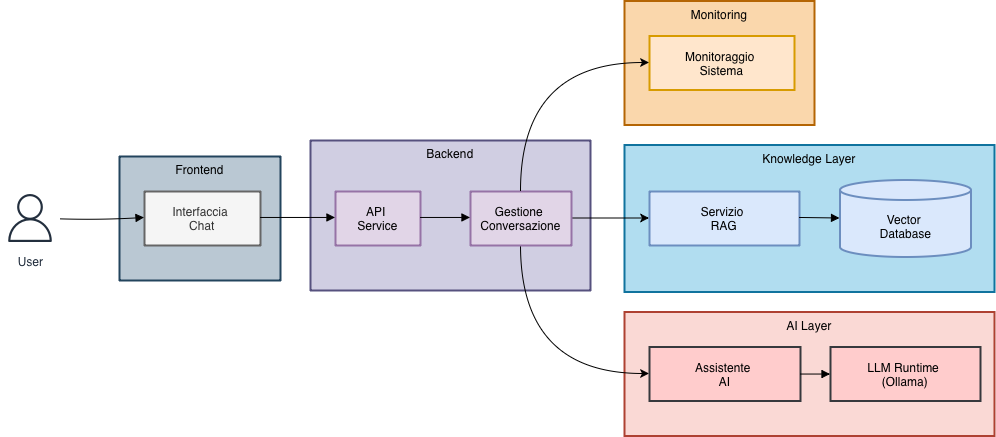
\includegraphics[width=0.75\textwidth]{chapter2/images/intre_usecase.png}
  \caption{Diagramma del caso d'uso ``Intré'': attori, interazioni principali e
    confini del sistema.}
  \label{fig:intre_usecase}
\end{figure}

\subsection{Scenario applicativo}
\label{subsec:application_scenario}

Lo scenario operativo previsto per il prototipo si colloca nel flusso già
presente in i3Guild. La Figura~\ref{fig:i3guild_guilds_list_screenshot} mostra
la consultazione dell'archivio delle Gilde, mentre la
Figura~\ref{fig:i3guild_guild_detail_screenshot} riporta il dettaglio di una
singola Gilda. La Figura~\ref{fig:i3guild_rag_screenshot} mostra invece il
punto in cui l'utente interroga l'assistente RAG in linguaggio naturale. La
sequenza rende visibile sia la sorgente applicativa da cui viene costruito il
corpus sia il punto in cui il prototipo espone il retrieval all'interno
dell'interfaccia.

\begin{figure}[ht]
  \centering
  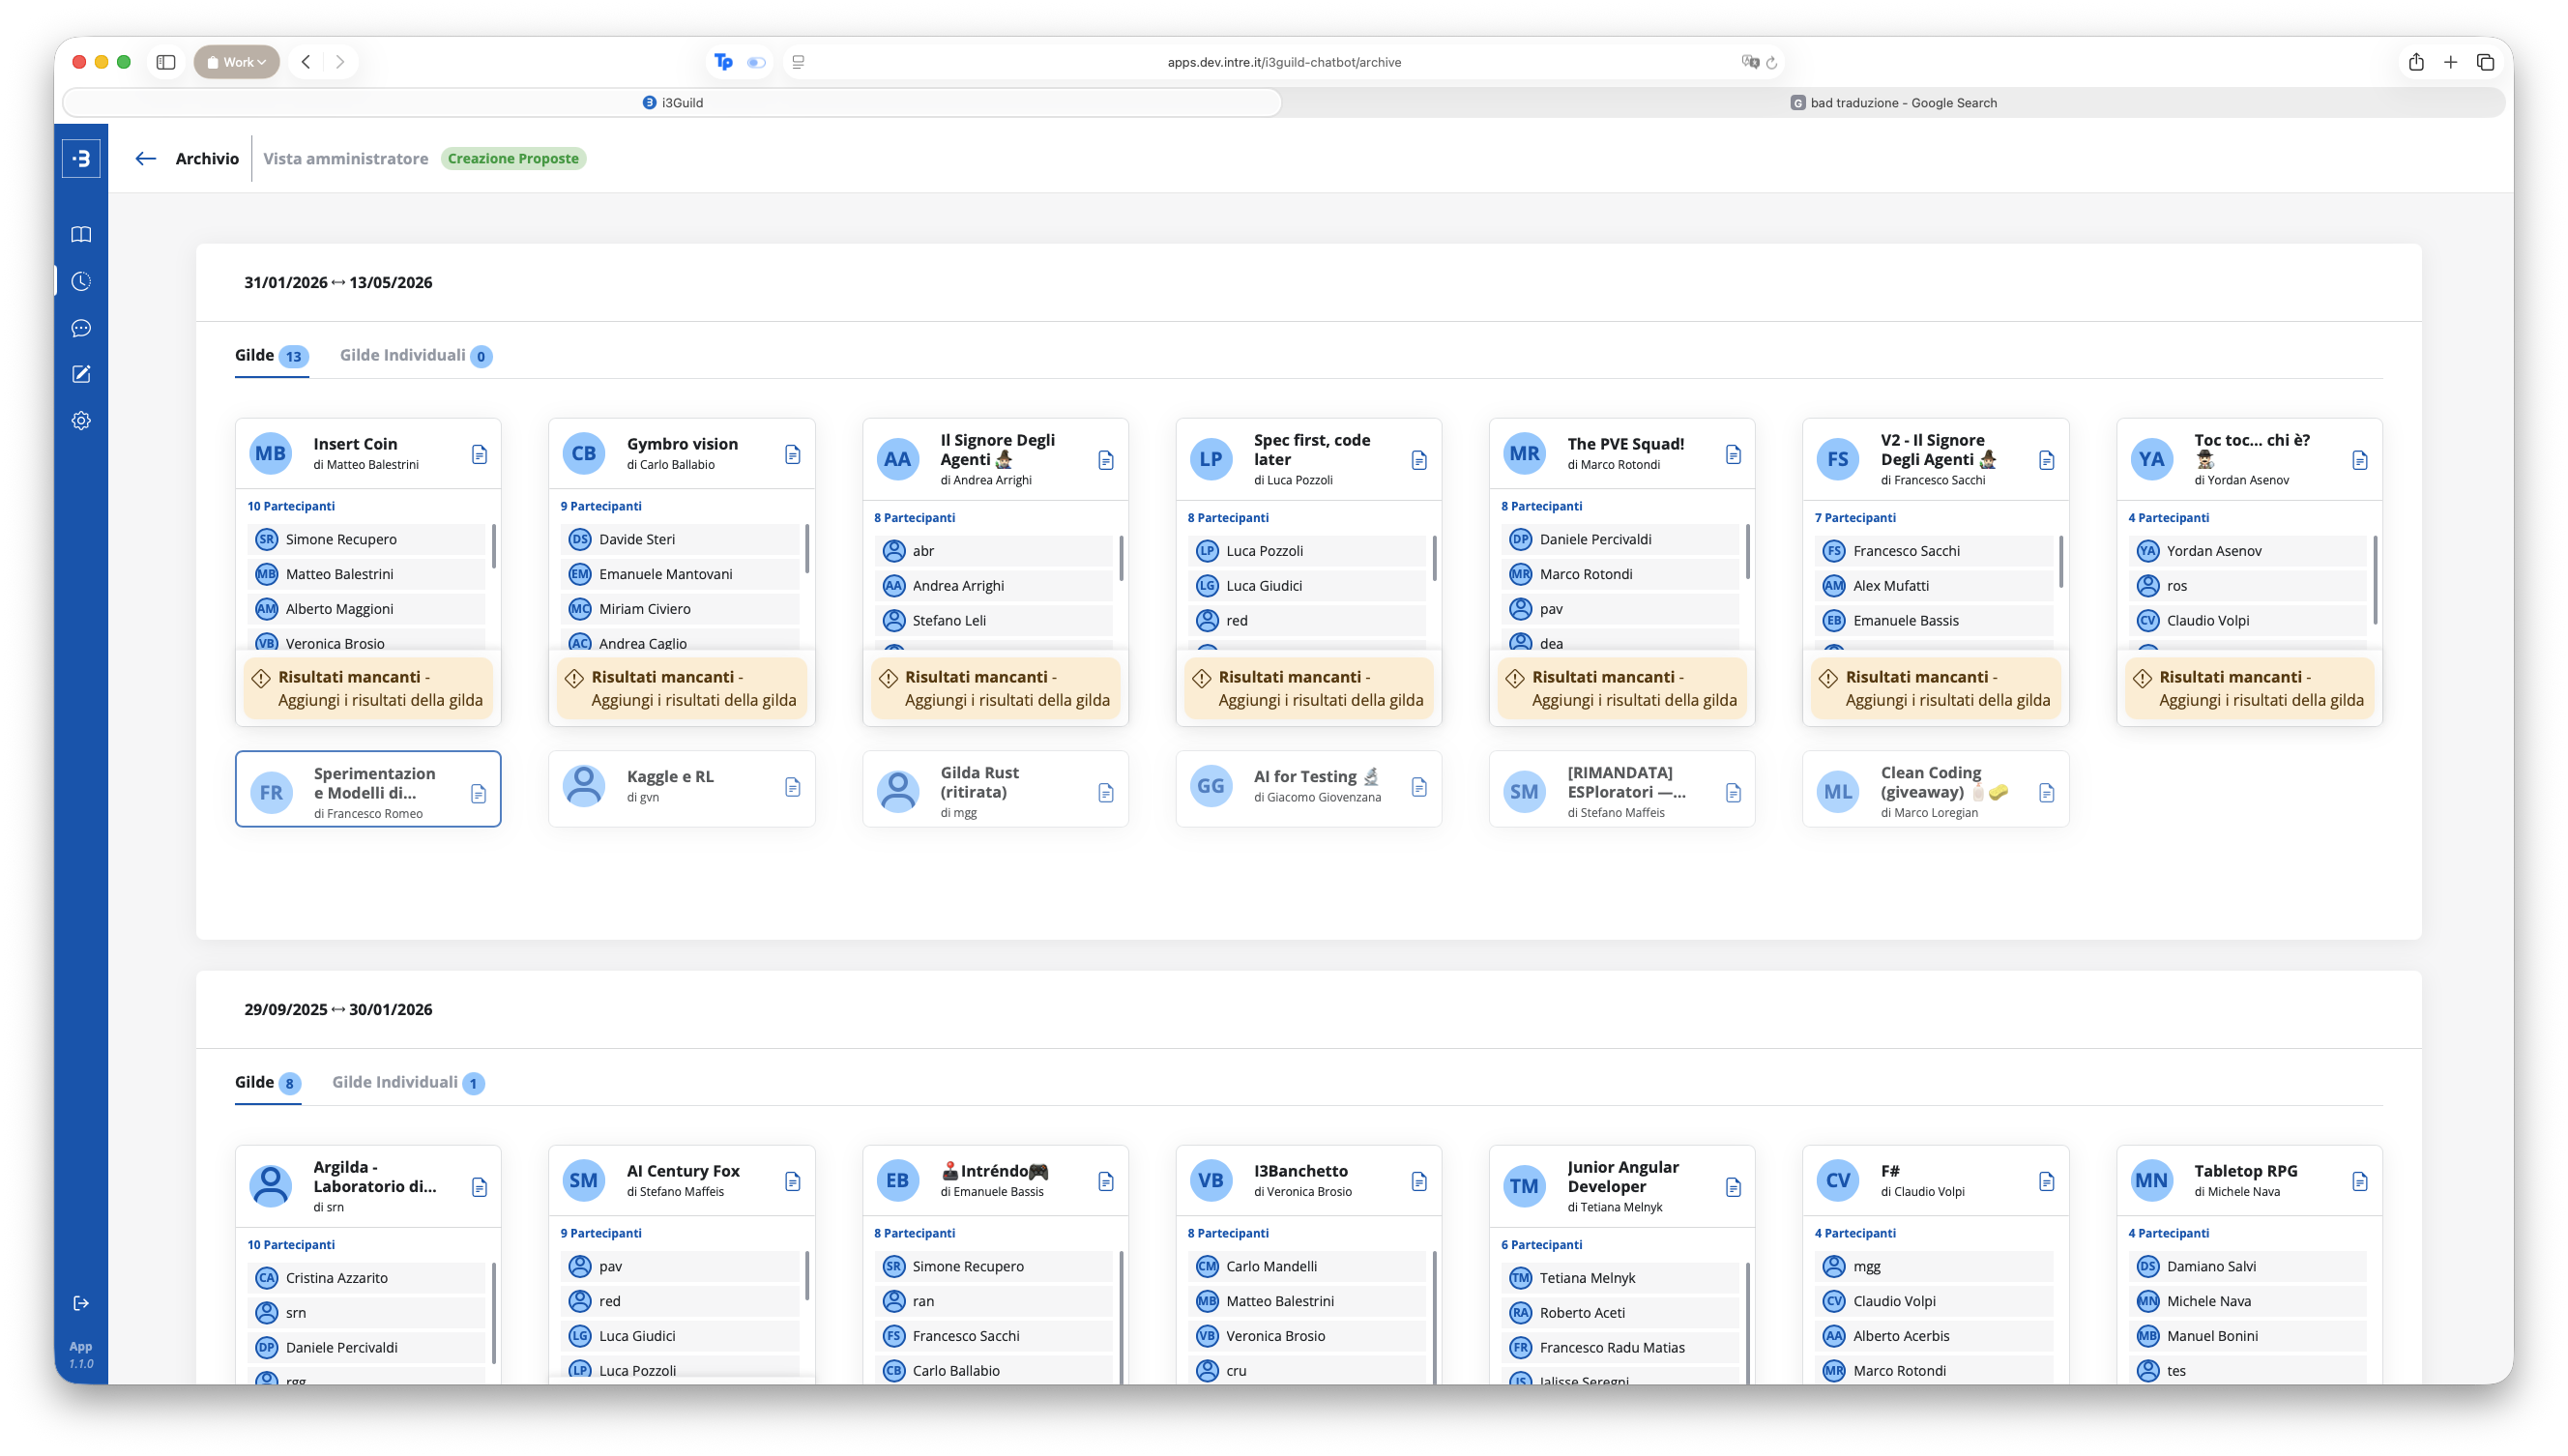
\includegraphics[width=0.95\textwidth]{chapter2/images/gilde.png}
  \caption{Vista dell'archivio delle Gilde nell'interfaccia i3Guild. La
    schermata mostra il punto di accesso al corpus applicativo usato dal
    sistema RAG.}
  \label{fig:i3guild_guilds_list_screenshot}
\end{figure}

\begin{figure}[ht]
  \centering
  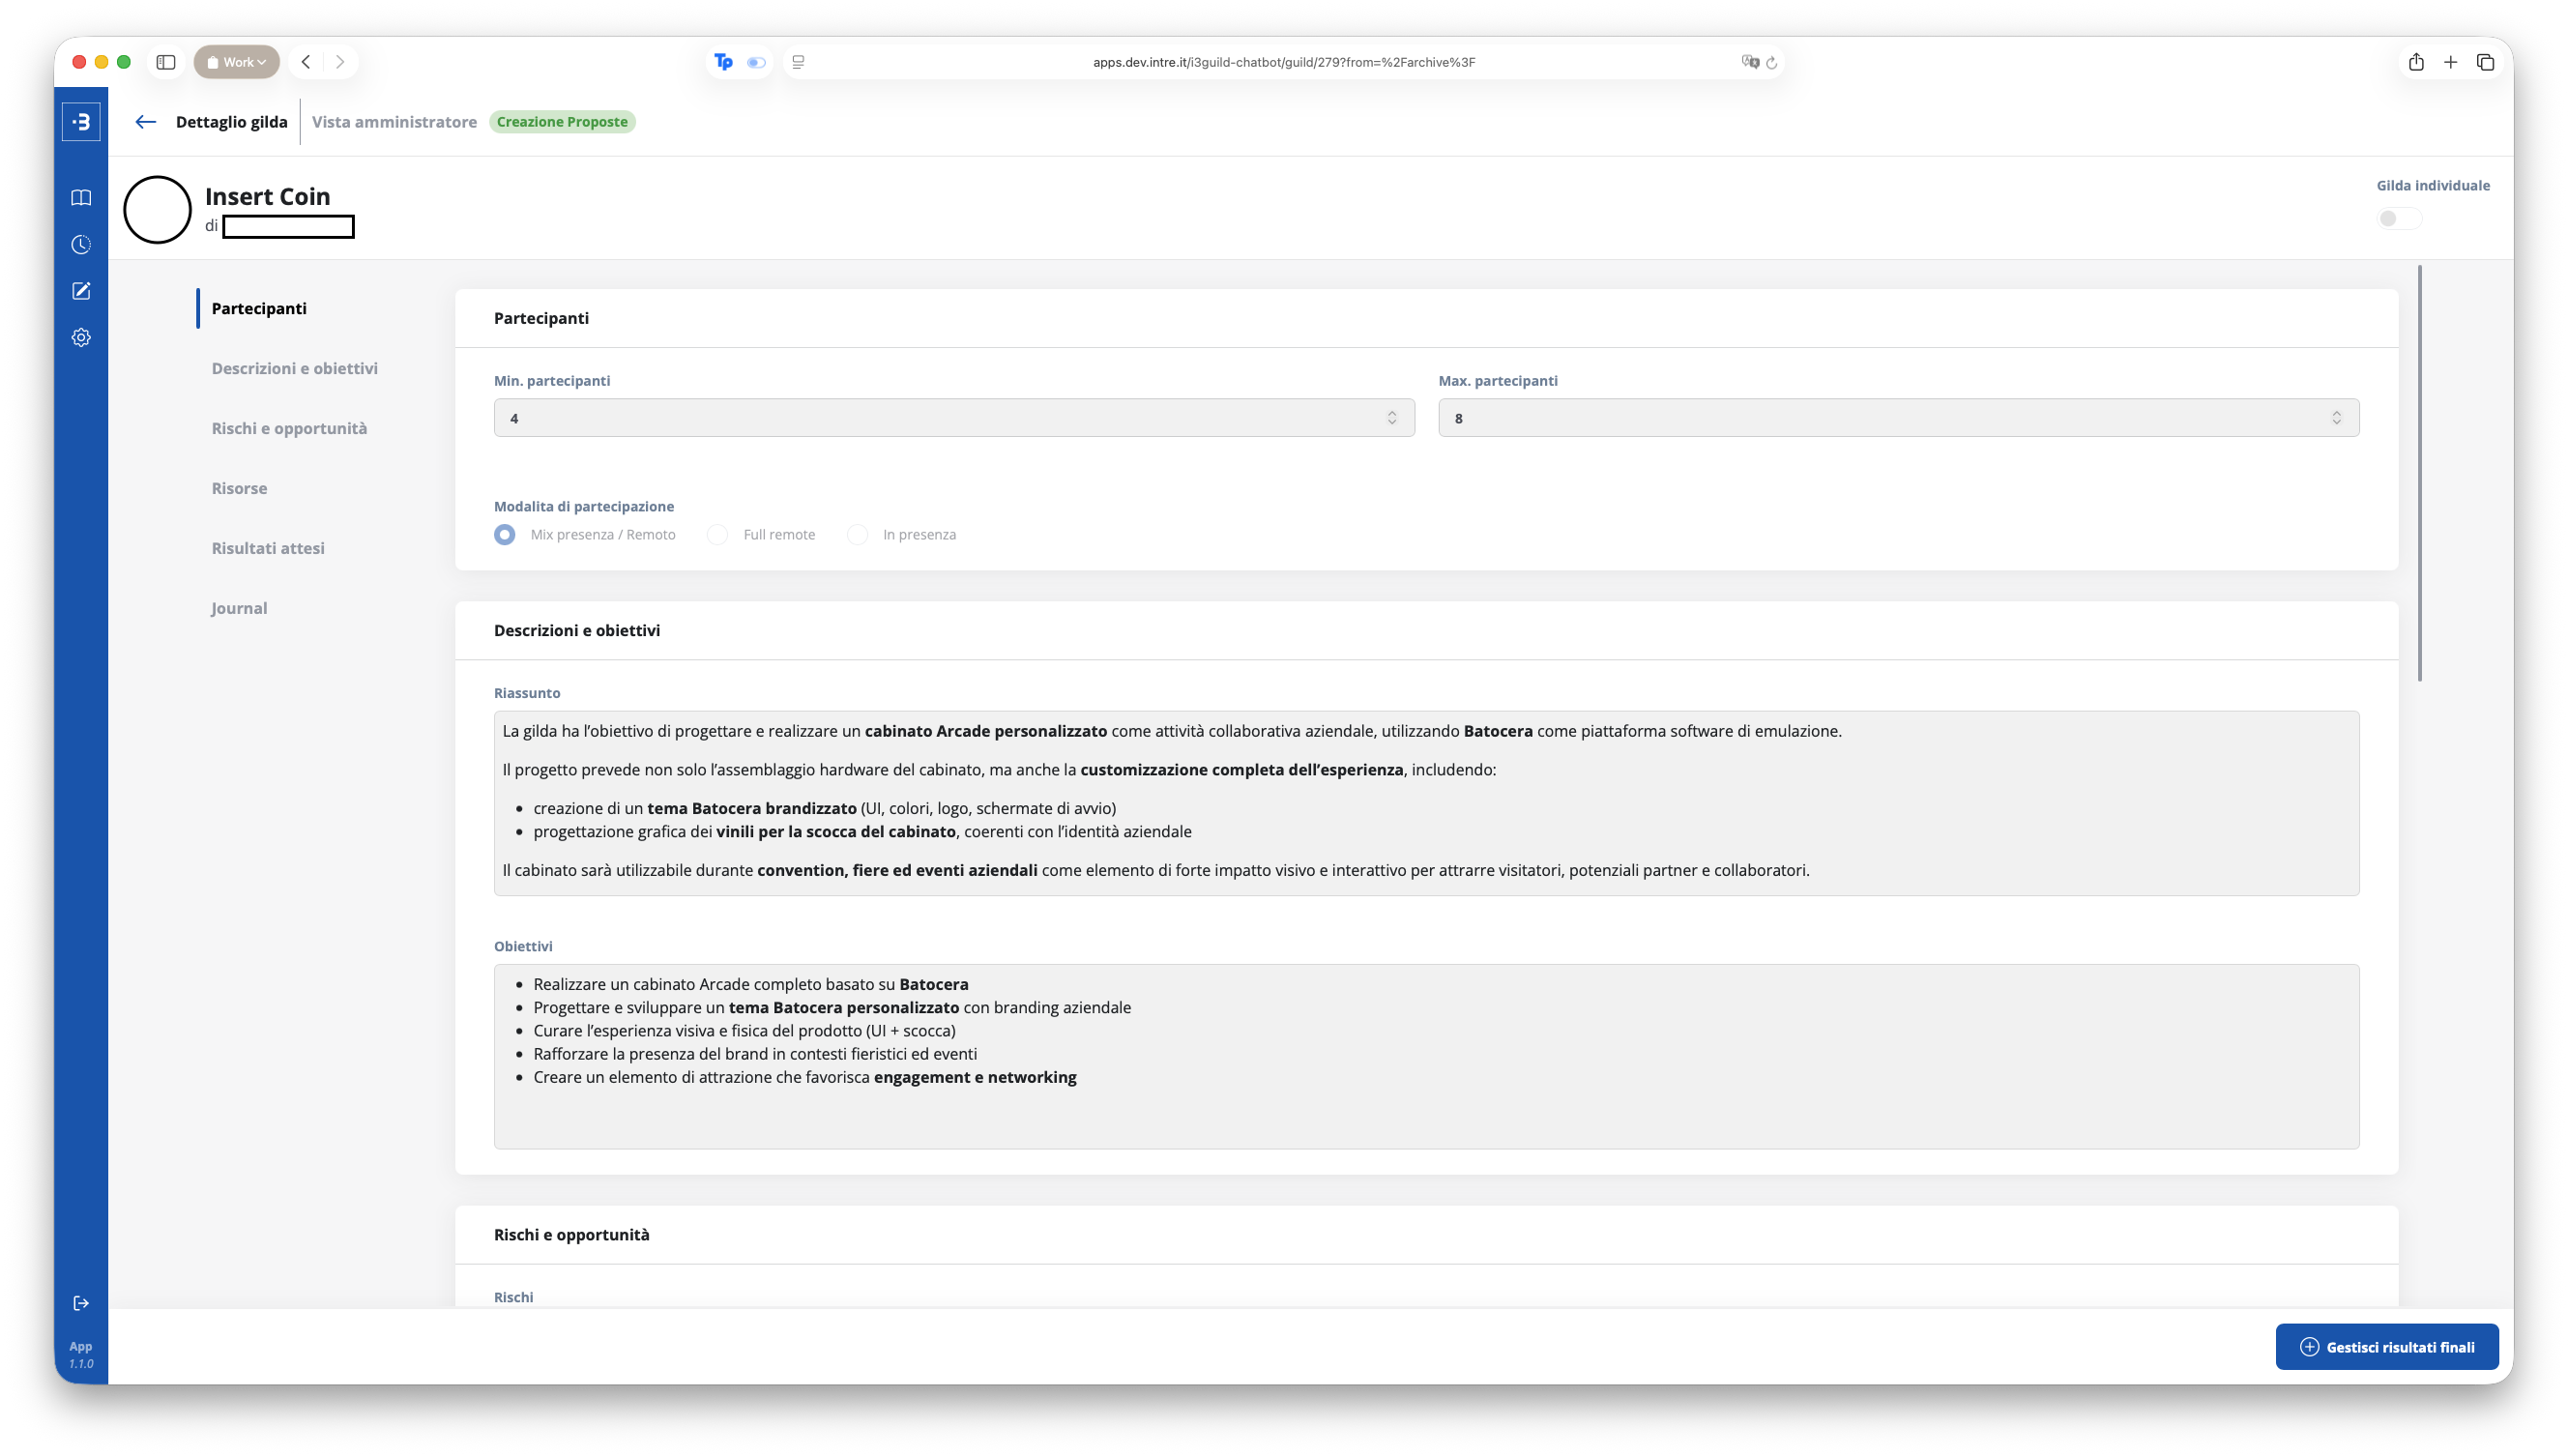
\includegraphics[width=0.95\textwidth]{chapter2/images/esempio_gilda.png}
  \caption{Dettaglio di una Gilda in i3Guild. I campi descrittivi e i metadati
    visualizzati nella pagina costituiscono parte delle informazioni trasformate
    in documenti indicizzabili.}
  \label{fig:i3guild_guild_detail_screenshot}
\end{figure}

\begin{figure}[ht]
  \centering
  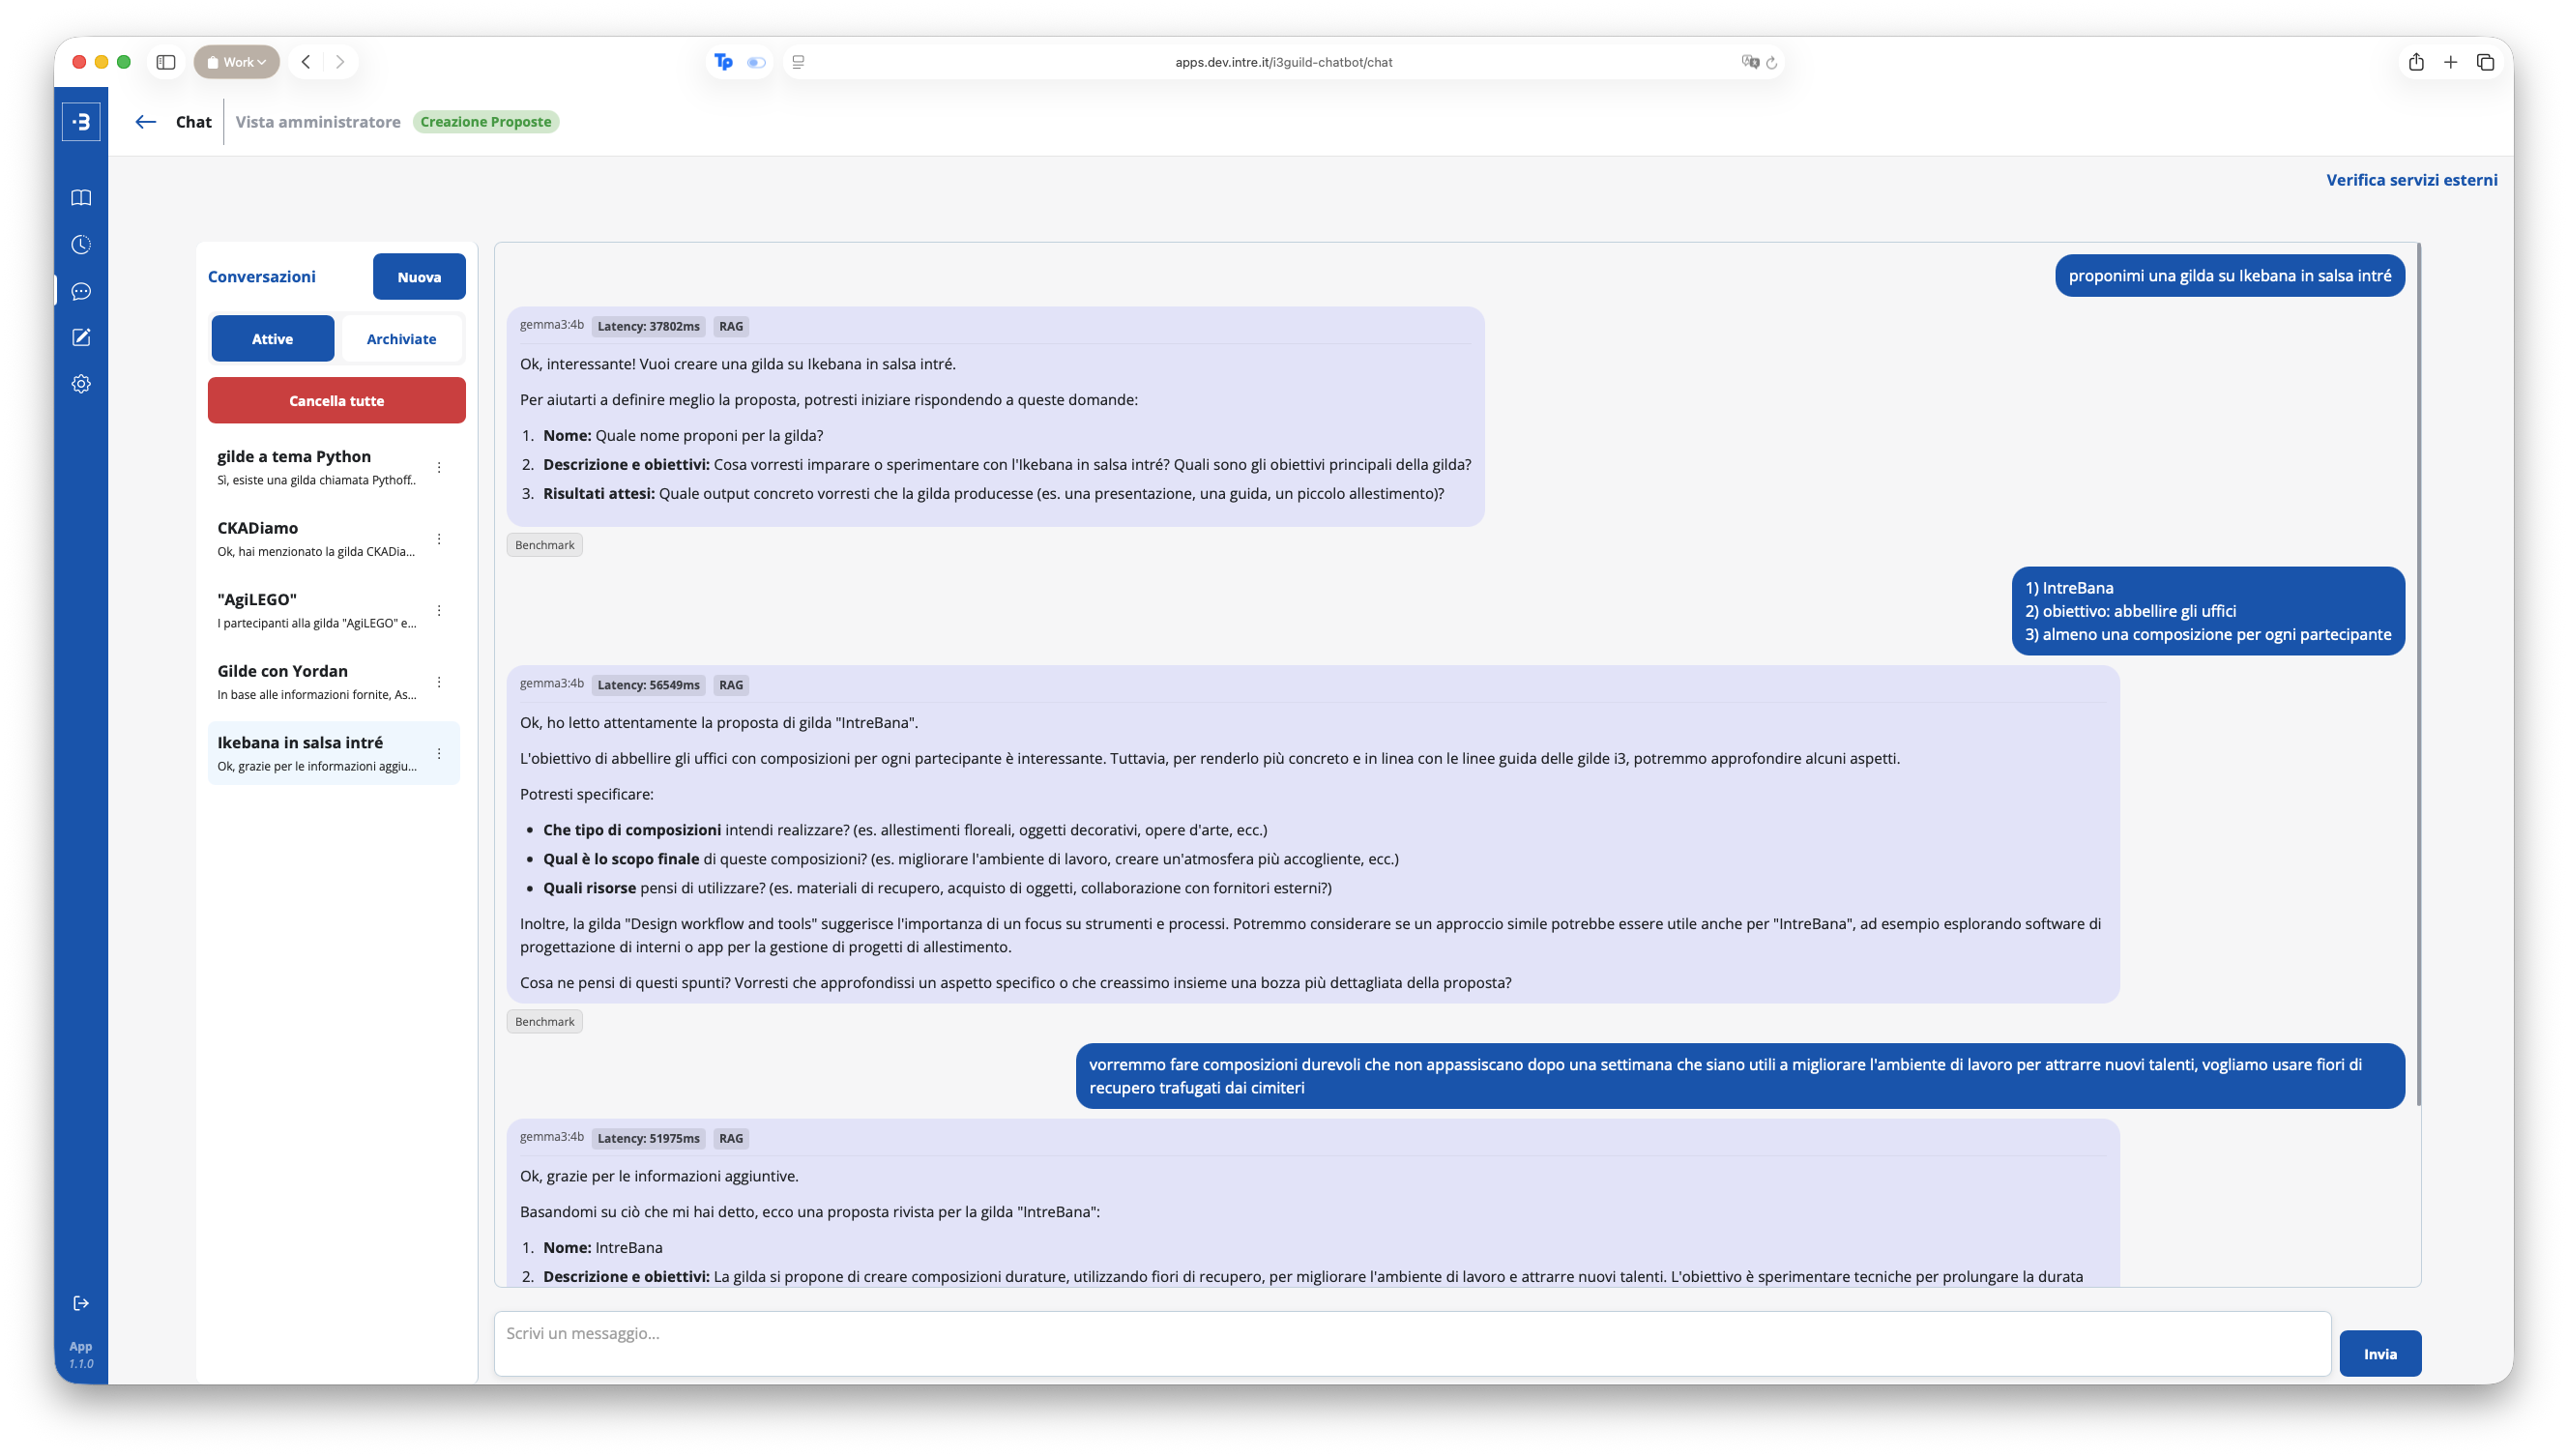
\includegraphics[width=0.95\textwidth]{chapter2/images/chat.png}
  \caption{Esempio di interazione con l'assistente RAG integrato in i3Guild.
    La schermata mostra la consultazione in linguaggio naturale del corpus e il
    collegamento tra risposta generata e informazioni recuperate.}
  \label{fig:i3guild_rag_screenshot}
\end{figure}

% -------------------------------------------------------------
\section{Requisiti di sistema}
\label{sec:system_requirements}
% -------------------------------------------------------------

Il caso d'uso appena descritto permette di passare dalla motivazione generale ai
requisiti del sistema. Essi sono stati ricavati dall'analisi del corpus, dai
vincoli infrastrutturali di Intré e dalle policy aziendali in materia di
protezione dei dati. La Tabella~\ref{tab:req_summary} sintetizza i requisiti ad
alto livello, suddivisi per categoria.

\begin{table}[ht]
  \centering
  \caption{Riepilogo requisiti ad alto livello.}
  \label{tab:req_summary}
  \small
  \begin{tabular}{p{3.5cm}p{9.5cm}}
    \toprule
    \textbf{Categoria} & \textbf{Requisiti principali} \\
    \midrule
    Funzionali & Ricerca semantica full-text su documenti interni; generazione
      di risposte contestualizzate con riferimenti alle fonti; capacità di
      filtraggio per metadati (epoca, modalità di partecipazione, proprietario
      della gilda). \\
    \addlinespace
    Privacy e conformità & Esecuzione on-premise; nessun invio di dati a
      servizi cloud esterni; logging e auditing degli accessi; protezione dei
      dati in conformità al GDPR~\cite{gdpr2016}. I rischi relativi alla
      privacy nei sistemi RAG, tra cui la possibile estrazione dei dati di
      retrieval, sono discussi in letteratura~\cite{zeng2024privacy}; la
      scelta on-premise costituisce la principale misura mitigativa adottata. \\
    \addlinespace
    Performance & Latenza compatibile con uso interattivo per query semplici,
      distinguendo tra modello già caricato e cold start; throughput adeguato a
      carichi concorrenti moderati; inferenza CPU-only come scenario primario. \\
    \addlinespace
    Costi e sostenibilità & Minimizzazione dei costi operativi tramite uso
      efficiente delle risorse (quantizzazione dei modelli, inferenza CPU);
      adozione di soluzioni open-source senza costi per licenze. \\
    \addlinespace
    Manutenibilità & Componenti modulari con interfacce standardizzate;
      automazione della pipeline di ingestione; documentazione e test
      automatizzati. \\
    \bottomrule
  \end{tabular}
\end{table}

\subsection{Vincoli architetturali}
\label{subsec:constraints}

I requisiti precedenti si traducono in vincoli architetturali non negoziabili.
L'esecuzione on-premise è il vincolo più rilevante: i dati delle Gilde, incluse
le informazioni sui partecipanti e sui progetti, non possono transitare su
infrastrutture cloud di terze parti. Il deployment locale diventa quindi la
condizione tecnica per rispettare i principi di integrità e riservatezza
previsti dal GDPR~\cite{gdpr2016}. L'integrazione deve inoltre rimanere
compatibile con lo stack i3Guild esistente, basato su Docker Compose,
PostgreSQL/Prisma, Next.js e Keycloak per l'autenticazione.

Un vincolo meno visibile, ma altrettanto determinante, riguarda le risorse
hardware. L'ambiente Docker dispone di 8~GB di RAM complessivi, condivisi tra
database, servizi applicativi, pipeline di embedding quando attiva e modello di
generazione del testo. Questa disponibilità limita la scelta del modello LLM,
discussa nella Sezione~\ref{subsec:llm_choice}, e impone di evitare componenti
con requisiti di memoria elevati. Per la stessa ragione, generazione ed
embedding devono restare locali senza fare affidamento su API esterne: Ollama
gestisce il modello generativo, mentre FastEmbed/Haystack produce gli embedding
senza dipendere da provider cloud.

% -------------------------------------------------------------
\section{Scelte tecnologiche e confronto}
\label{sec:tech_choices}
% -------------------------------------------------------------

Le scelte tecnologiche sono state effettuate a partire dai vincoli appena
definiti. Per ciascun componente principale dello stack sono state valutate
alternative compatibili con l'esecuzione on-premise, privilegiando soluzioni
semplici da integrare nello stack i3Guild, osservabili e sostenibili rispetto
alle risorse disponibili.

\subsection{Framework di orchestrazione RAG}
\label{subsec:framework_choice}

Il framework di orchestrazione deve collegare ingestione, embedding, retrieval
e generazione senza introdurre eccessiva complessità operativa. Sono stati
considerati tre framework open-source: \textbf{LangChain},
\textbf{LlamaIndex} e \textbf{Haystack~2.x}.

\paragraph{LangChain} offre l'ecosistema più ampio di integrazioni e una forte
vocazione verso workflow agentici e \textit{multi-step reasoning}. LangGraph ha
ampliato questa impostazione, permettendo di modellare applicazioni multi-agente
come grafi di stato. Tale flessibilità è utile in scenari complessi, ma nel progetto
in esame introduce un costo non trascurabile in termini di curva di
apprendimento, stabilità delle API e manutenzione, anche alla luce dei
\textit{breaking changes} frequenti.

\paragraph{LlamaIndex} è orientato alla gestione dei dati e al retrieval
avanzato. Offre numerosi data connector e strutture di indicizzazione
specializzate, risultando particolarmente adatto a pipeline di
question-answering documentale. Rispetto al caso
considerato, tuttavia, l'obiettivo principale non è solo indicizzare sorgenti
eterogenee, ma integrare una pipeline osservabile e facilmente testabile nello
stack applicativo esistente.

\paragraph{Haystack 2.x} (deepset) adotta un modello a componenti tipizzati
con input/output espliciti, organizzati in pipeline dichiarative serializzabili
in YAML. La sua politica pipeline-first favorisce la tracciabilità, i test e
la sostituzione dei componenti in produzione, aspetti più rilevanti per il
prototipo rispetto alla disponibilità di astrazioni agentiche avanzate.
La Tabella~\ref{tab:framework_comparison} sintetizza il confronto tra i tre
framework considerati rispetto ai criteri più rilevanti per il prototipo.

\begin{table}[ht]
  \centering
  \caption{Confronto sintetico dei framework RAG candidati.}
  \label{tab:framework_comparison}
  \small
  \begin{tabularx}{\textwidth}{L{2.8cm}YYY}
    \toprule
    \textbf{Criterio} & \textbf{LangChain} & \textbf{LlamaIndex} &
      \textbf{Haystack 2.x} \\
    \midrule
    Filosofia & Agente/imperativa & Data-first & Pipeline dichiarativa \\
    Orientamento operativo & Workflow agentici e catene applicative &
      Indicizzazione e gestione dati & Pipeline RAG dichiarative \\
    Integrazione Qdrant & Nativa & Nativa & Nativa \\
    Integrazione Ollama & Sì & Sì & Sì \\
    Testabilità pipeline & Media & Media & Alta \\
    Serializzazione YAML & No & Parziale & Sì \\
    Adatto per produzione RAG & Sì (con overhead) & Sì & Sì (preferito) \\
    \bottomrule
  \end{tabularx}
\end{table}

\noindent Alla luce di questo confronto, Haystack 2.x risulta la soluzione più
coerente con il progetto. L'architettura a componenti tipizzati, la
documentazione rigorosa, le integrazioni native con Qdrant
(\texttt{QdrantDocumentStore}), FastEmbed per embedding densi e sparsi e Ollama
per la generazione permettono di costruire una pipeline osservabile senza
introdurre un framework agentico più complesso del necessario. La possibilità di
serializzare le pipeline rafforza questa scelta in un sistema RAG orientato alla
produzione e vincolato all'esecuzione on-premise.

\subsection{Database vettoriale}
\label{subsec:vectordb_choice}

La ricerca di similarità approssimata (\emph{Approximate Nearest Neighbor},
ANN) su vettori ad alta dimensionalità è il componente infrastrutturale che
abilita il retrieval. La scelta del database vettoriale incide su latenza,
filtraggio per metadati, semplicità di deployment e capacità di manutenzione
dell'indice; per questo sono stati valutati quattro database vettoriali
self-hostable.
La Tabella~\ref{tab:vectordb_comparison} mostra il confronto usato per
motivare la scelta di Qdrant.

\begin{table}[ht]
  \centering
  \caption{Analisi comparativa dei database vettoriali candidati.}
  \label{tab:vectordb_comparison}
  \small
  \begin{tabularx}{\textwidth}{L{1.5cm}L{1.5cm}L{1.4cm}YYY}
    \toprule
    \textbf{Database} & \textbf{Impl.} & \textbf{Indice} &
      \textbf{Filtering} & \textbf{Dashboard} & \textbf{Deployment} \\
    \midrule
    \textbf{Qdrant} & Rust & HNSW & Pre-filtering payload & Web UI &
      1 container \\
    pgvector & C & IVFFlat / HNSW & SQL \texttt{WHERE} & No &
      Estensione PG \\
    Milvus & Go/C++ & HNSW, IVF & Attribute-based & Attu &
      Multi-container \\
    Chroma & Python & HNSW (hnswlib) & Metadata base & No & 1 container \\
    \bottomrule
  \end{tabularx}
\end{table}

Il confronto non si limita alle prestazioni pure: nel contesto i3Guild hanno
peso anche la semplicità operativa e la possibilità di applicare filtri sui
metadati delle Gilde. I principali criteri di esclusione e selezione sono i
seguenti:

\begin{itemize}
  \item \textbf{pgvector} è stato considerato in quanto l'infrastruttura
    i3Guild utilizza già PostgreSQL. Tuttavia, la letteratura segnala che le
    prestazioni di pgvector degradano significativamente oltre le centinaia di
    migliaia di vettori, con ritardi fino a 15 volte superiori rispetto a
    Qdrant in termini di throughput su dataset grandi. In questo progetto hanno
    pesato soprattutto l'assenza di una dashboard integrata e di un payload
    filtering flessibile, che avrebbero reso meno diretta la gestione dei
    metadati delle Gilde.
  \item \textbf{Milvus} è stato escluso per l'elevata complessità di deploy:
    richiede componenti aggiuntivi (\texttt{etcd}, \texttt{MinIO}), aumentando
    il carico operativo incompatibile con i vincoli del progetto.
  \item \textbf{Chroma} è implementato in Python e soffre di instabilità della
    persistenza dati nelle versioni precedenti; è più adatto a prototipi
    che a sistemi di produzione.
  \item \textbf{Qdrant} è scritto in Rust e offre buone prestazioni con latenze
    stabili nei benchmark disponibili. La funzionalità di pre-filtering, che
    applica i filtri sui payload \emph{prima} della ricerca vettoriale, è
    particolarmente rilevante per query
    contestuali come ``gilda dell'epoca X'': il filtering riduce lo spazio di
    ricerca prima del calcolo ANN, mantenendo il top-$K$ accurato. Offre Web
    UI integrata su porta 6333, client TypeScript ufficiale compatibile con
    Next.js e deploy in singolo container Docker.
\end{itemize}

\noindent Per le ragioni discusse, e in particolare per il bilanciamento tra
prestazioni, semplicità di deployment e supporto al filtering sui metadati,
Qdrant è stato selezionato come database vettoriale del progetto. La scelta è
coerente con il vincolo aziendale di self-hosting e con la necessità di
mantenere il sistema manutenibile anche in un contesto prototipale.

\subsection{Modello di embedding}
\label{subsec:embedding_choice}

Il modello di embedding converte i documenti testuali in rappresentazioni
numeriche interrogabili da Qdrant. Nel progetto questa funzione è separata
dall'inferenza generativa: Ollama serve il modello di chat, mentre FastEmbed,
tramite Haystack, produce le rappresentazioni usate per l'indicizzazione. La
pipeline genera sia embedding densi sia embedding sparsi, così il retrieval può
combinare similarità semantica e corrispondenza lessicale su nomi propri,
tecnologie e termini ricorrenti nelle Gilde.

\begin{table}[ht]
  \centering
  \caption{Configurazione embedding del sistema RAG.}
  \label{tab:embedding_models}
  \small
  \begin{tabular}{L{2.7cm}L{4.1cm}L{3cm}L{3.6cm}}
    \toprule
    \textbf{Ruolo} & \textbf{Componente Haystack} & \textbf{Default} &
      \textbf{Funzione} \\
    \midrule
    Embedding denso & Document/text embedder denso &
      \makecell[l]{\texttt{paraphrase-}\\\texttt{multilingual-}\\\texttt{mpnet-base-v2}} &
      Similarità semantica tra query e documenti. \\
    Embedding sparso & Document/text embedder sparso & \makecell[l]{\texttt{prithivida/}\\\texttt{Splade\_PP\_en\_v1}} &
      Matching lessicale pesato, utile per termini specifici. \\
    Store ibrido & \breakcode{QdrantDocumentStore} con
      \breakcode{use_sparse_embeddings=true} & \breakcode{i3guild_knowledge} &
      Persistenza con vettori densi e rappresentazioni sparse. \\
    \bottomrule
  \end{tabular}
\end{table}

\noindent La separazione tra indicizzazione e generazione riduce
l'accoppiamento operativo: Ollama rimane dedicato alla risposta LLM, mentre il
job batch produce gli embedding senza dipendere dal server di chat. La
componente sparsa rende inoltre il retrieval meno dipendente dalla sola
similarità densa, aspetto rilevante in un corpus dove nomi propri, tecnologie e
termini ricorrenti hanno spesso valore informativo letterale. Ingestione e query
seguono quindi lo stesso schema operativo: in scrittura vengono generati
embedding densi e sparsi dei documenti; in lettura la query viene trasformata
nelle due rappresentazioni corrispondenti e inviata al retriever ibrido Qdrant.
Il valore
\texttt{EMBEDDING\_DIMENSIONS=768} rimane il riferimento per la componente
densa.

La scelta della ricerca ibrida non deriva da una valutazione quantitativa
condotta sul corpus i3Guild, perché durante il progetto non è stato costruito
un dataset annotato con query e documenti rilevanti. È però coerente con
evidenze esterne recenti: nei task RAG di TREC 2025 un sistema sparse+dense con
reranking ottiene i migliori risultati riportati dal team NITATREC
(\textit{MAP} 0.1037, \textit{nDCG@30} 0.527 e \textit{Recall@100}
0.158)~\cite{sinha2025nitatrec}; in un benchmark finanziario su documenti misti
testo-tabella, una pipeline a due stadi con retrieval ibrido e reranking
raggiunge \textit{Recall@5} 0.816 e \textit{MRR@3} 0.605, superando i metodi
single-stage~\cite{akarsu2026bm25correctiverag}. Altri studi mostrano però che
il vantaggio non è universale: nel dominio biomedicale una baseline densa resta
molto competitiva e le differenze tra strategie dipendono dal corpus e dalle
metriche considerate~\cite{bal2026biomedicalretrieval}. Per i3Guild questi
risultati vanno quindi usati come supporto alla scelta progettuale, non come
prova sperimentale locale: la componente sparsa è motivata soprattutto dalla
presenza di nomi di Gilde, ruoli, modalità di partecipazione e termini tecnici
che hanno valore informativo letterale.

\subsection{Server di inferenza LLM e selezione del modello di chat}
\label{subsec:llm_choice}

Il componente di generazione del testo è gestito da \textbf{Ollama}, server di
inferenza locale che supporta modelli in formato GGUF e consente l'uso di
varianti quantizzate a 4 e 8 bit. Nel prototipo aziendale la scelta del modello
di chat è stata condizionata da un vincolo operativo preciso: l'intero stack
Docker dispone di risorse limitate e deve eseguire, nello stesso ambiente,
PostgreSQL, Qdrant, il servizio Next.js, la pipeline RAG e Ollama. Per questo
la selezione non mira a identificare il modello migliore in senso assoluto, ma
un modello sufficientemente stabile per validare l'integrazione end-to-end.

\noindent Il modello adottato nel prototipo è \texttt{gemma3:4b}, distribuito
in Ollama come \texttt{gemma3:latest}. La scelta deriva da prove preliminari
interne su modelli disponibili nel registry Ollama, valutati rispetto a latenza
percepita, consumo di memoria e qualità minima delle risposte in presenza di
contesto RAG. Il modello resta caricabile nello stesso ambiente dei servizi
PostgreSQL, Qdrant, Next.js e FastAPI, ma offre un margine qualitativo maggiore
rispetto a modelli da circa 1B parametri. Le risposte non sono usate come prova
generale della qualità del modello; sono sufficienti per validare il flusso
applicativo quando il contesto recuperato da Qdrant è pertinente.

Le prove locali hanno confrontato dodici modelli Ollama su 14 query, divise tra
prompt generali e prompt RAG. La valutazione manuale ha assegnato tre punteggi
per accuratezza o fedeltà, pertinenza e coerenza. I risultati non costituiscono
un benchmark scientifico, perché il numero di query è ridotto e il carico della
macchina non è stato isolato; sono però utili come criterio progettuale. In
media, \texttt{gemma3:1b} ha mostrato la latenza totale più bassa
(\(\approx 6.7\) s) e un buon throughput (\(\approx 28\) parole/s), ma una
coerenza più debole nelle risposte RAG. \texttt{gemma3:4b} ha richiesto più
tempo (\(\approx 17.3\) s in media), mantenendo però il punteggio medio più alto
tra i modelli di dimensione compatibile con il prototipo. Modelli ragionativi
come \texttt{phi4-mini-reasoning} hanno prodotto latenze troppo elevate per
l'uso interattivo, mentre alcune alternative molto compatte hanno mostrato
output meno controllabili. La scelta di \texttt{gemma3:4b} privilegia quindi un
compromesso pratico: qualità sufficiente, integrazione immediata in Ollama e
risorse ancora compatibili con l'ambiente condiviso.

\noindent Questa valutazione resta volutamente interna al progetto aziendale:
serve a rendere eseguibile il prototipo i3Guild, non a produrre conclusioni
generali sull'inferenza locale. La generalizzazione del problema, cioè la misura
sistematica di memoria, cold start, \emph{time-to-first-token}, throughput e
impatto della quantizzazione su Apple Silicon, viene affrontata nei
Capitoli~\ref{chap:ottimizzazione} e~\ref{chap:evaluation}.

% -------------------------------------------------------------
\section{Proposta architetturale}
\label{sec:architecture}
% -------------------------------------------------------------

Le scelte tecnologiche descritte portano a un'architettura modulare e
containerizzata, in cui ingestione e normalizzazione dei dati, generazione degli
embedding, persistenza vettoriale, retrieval e inferenza tramite LLM restano
fasi operative distinte. Questa separazione rende i componenti più facili da
monitorare e sostituire, mantenendo l'integrazione coerente con lo stack
i3Guild. La Figura~\ref{fig:architecture} mostra lo schema generale
dell'architettura.

\begin{figure}[ht]
  \centering
  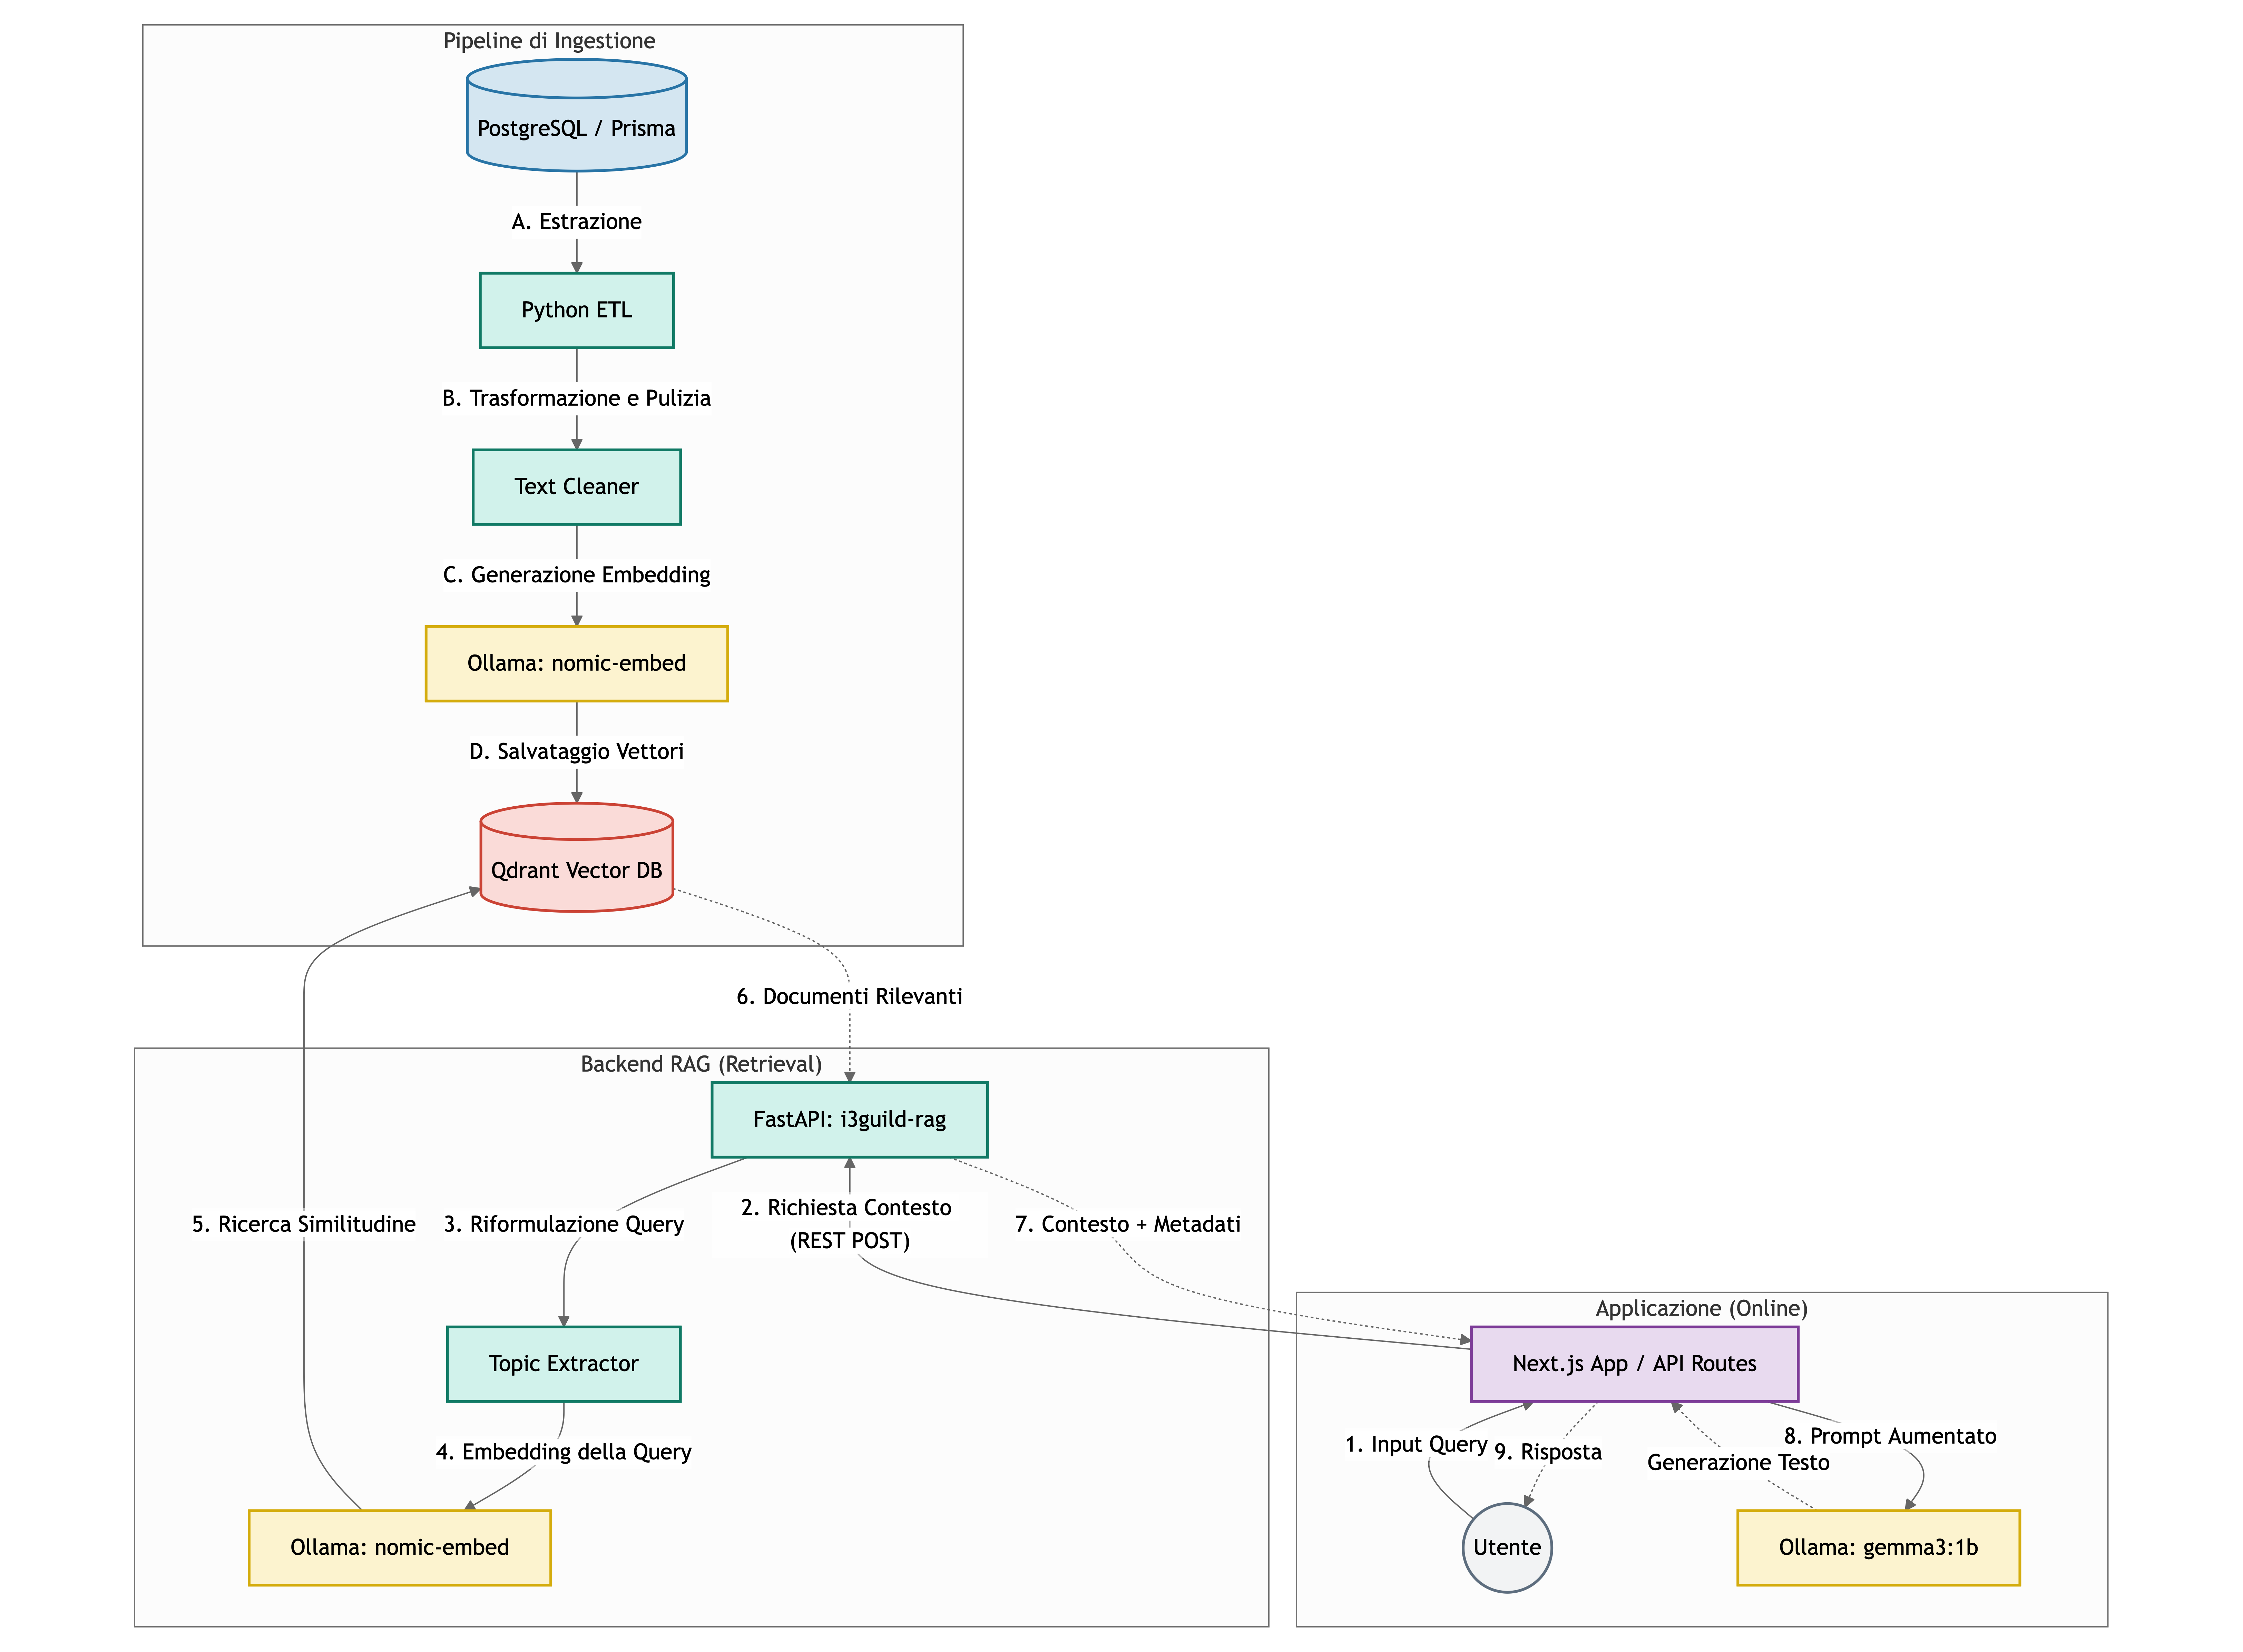
\includegraphics[width=0.85\textwidth]{chapter2/images/architecture_diagram.png}
  \caption{Schema architetturale del sistema RAG on-premise per i3Guild.
    Il flusso di ingestione (ETL) popola Qdrant a partire da PostgreSQL;
    il flusso di retrieval serve le query di Next.js tramite FastAPI.}
  \label{fig:architecture}
\end{figure}

\subsection{Componenti principali}
\label{subsec:components}

I componenti non sono separati soltanto per ragioni di deployment: ciascuno
risponde a un requisito emerso nelle sezioni precedenti. PostgreSQL rimane la
sorgente autoritativa dei dati; Qdrant rende interrogabile il corpus per
similarità; Ollama consente di mantenere la generazione in locale; FastAPI
espone verso Next.js un confine applicativo chiaro, senza incorporare la logica
RAG direttamente nel frontend.

\begin{description}
  \item[Ingestione e pre-processing]
    Pipeline batch Python che esegue le fasi ETL descritte nella
    Sezione~\ref{subsec:ingestion_pipeline}. Acquisisce i documenti da
    PostgreSQL, normalizza il testo, esegue il chunking, genera embedding densi
    e sparsi con FastEmbed/Haystack e indicizza su Qdrant.

  \item[Strategia di chunking] Sulla base dell'analisi dei dati
    (Sezione~\ref{subsec:data_analysis}), viene adottato l'approccio a
    \emph{documento consolidato} (1 Gilda $\leftrightarrow$ 1 documento
    vettoriale): tutti i campi testuali rilevanti sono concatenati in un unico
    documento con separatori strutturati. Per gli outlier che superano il limite
    configurato viene applicato chunking con overlap, mantenendo nel chunk
    l'intestazione della Gilda. Questo approccio preserva il contesto semantico
    nella maggior parte dei casi e mantiene gestibili upsert e cancellazioni su
    Qdrant.

  \item[Database vettoriale (Qdrant)] Collection principale
    \texttt{i3guild\_knowledge} configurata per retrieval ibrido: vettore denso
    a 768 dimensioni, rappresentazione sparsa e payload JSON con metadati
    indicizzati per il filtering (Sezione~\ref{subsec:qdrant_collection}).

  \item[Orchestrazione RAG (Haystack 2.x)] Haystack è usato sia nel job di
    indicizzazione sia nel servizio di query. La pipeline batch collega gli
    embedder densi e sparsi con il writer; la pipeline di query usa i
    componenti corrispondenti e il retriever ibrido Qdrant.

  \item[Inference LLM (Ollama)] Server di inferenza locale; modello di chat
    adottato: \texttt{gemma3:4b}, selezionato sulla base di prove preliminari
    coerenti con i vincoli del prototipo
    (Sezione~\ref{subsec:llm_choice}).

  \item[Servizio API (FastAPI)] Microservizio Python che espone endpoint di
    retrieval e generazione, tra cui \texttt{POST /rag/retrieve} (porta 8000,
    mappata a 8002 su host). Restituisce documenti con score di similarità e
    campi diagnostici.

  \item[Osservabilità e sicurezza] Logging centralizzato, metriche di latenza
    e utilizzo risorse; autenticazione tramite Keycloak (già presente in
    i3Guild); cifratura a riposo per i dataset sensibili.
\end{description}

\subsection{Progettazione della collection Qdrant}
\label{subsec:qdrant_collection}

La collection \texttt{i3guild\_knowledge} è il punto in cui la conoscenza
estratta da i3Guild viene trasformata in indice interrogabile. La configurazione,
riportata nella Tabella~\ref{tab:qdrant_config}, supporta retrieval ibrido:
similarità vettoriale densa e componente sparsa nello stesso store.

\begin{table}[ht]
  \centering
  \caption{Parametri di configurazione della collection Qdrant.}
  \label{tab:qdrant_config}
  \small
  \begin{tabular}{L{4.2cm}L{3.5cm}L{5.5cm}}
    \toprule
    \textbf{Parametro} & \textbf{Valore} & \textbf{Motivazione} \\
    \midrule
    \breakcode{embedding_dim} & 768 & Dimensione della componente densa FastEmbed \\
    \breakcode{vectors.distance} & \breakcode{Cosine} & Standard per similarità
      semantica testuale \\
    \breakcode{use_sparse_embeddings} & \breakcode{true} & Abilita la componente
      sparsa per retrieval ibrido \\
    \breakcode{recreate_index} & \breakcode{true} (job batch) & Ricrea la
      collection ibrida mantenendo lo stesso nome \\
    \breakcode{hnsw_config.m} & 16 (default) & Compromesso velocità/precisione \\
    \breakcode{hnsw_config.ef_construct} & 100 (default) & Qualità dell'indice
      in fase di build \\
    \bottomrule
  \end{tabular}
\end{table}

Ogni punto nella collection porta un payload JSON con i campi elencati nella
Tabella~\ref{tab:qdrant_payload}, in particolare i campi marcati come indicizzati abilitano il
pre-filtering, caratteristica distintiva di Qdrant che applica i filtri sul
payload \emph{prima} della ricerca vettoriale, garantendo che il calcolo del
top-$K$ sia effettuato solo sul sottoinsieme filtrato.

\begin{table}[ht]
  \centering
  \caption{Struttura del payload Qdrant per la collection
    \texttt{i3guild\_knowledge}.}
  \label{tab:qdrant_payload}
  \small
  \begin{tabular}{L{3.7cm}L{2cm}L{5.8cm}L{1.4cm}}
    \toprule
    \textbf{Campo} & \textbf{Tipo} & \textbf{Descrizione} &
      \makecell[l]{\textbf{Ind.}} \\
    \midrule
    \breakcode{guild_id} & integer & ID della gilda sorgente & Sì \\
    \breakcode{guild_name} & keyword & Nome della gilda & Sì \\
    \breakcode{epoch_id} & integer & ID dell'epoca di appartenenza & Sì \\
    \breakcode{epoch_start} & datetime & Data inizio epoca & Sì \\
    \breakcode{epoch_end} & datetime & Data fine epoca (nullable) & Sì \\
    \breakcode{participation_mode} & keyword & FullRemote / Hybrid / OnSite & Sì \\
    \breakcode{is_individual} & bool & Gilda individuale & Sì \\
    \breakcode{owner_id} & keyword & ID del proprietario & Sì \\
    \breakcode{participants} & keyword[] & Nomi dei partecipanti & Sì \\
    \breakcode{participant_count} & integer & Numero di partecipanti & No \\
    \breakcode{source_text} & text & Testo originale del chunk & No \\
    \breakcode{last_synced} & datetime & Timestamp ultima sincronizzazione & No \\
    \bottomrule
  \end{tabular}
\end{table}

Gli ID dei documenti sono deterministici nel formato
\texttt{guild-\{guild\_id\}-chunk-\{index\}}. La reindicizzazione della stessa
Gilda produce quindi gli stessi identificativi e consente a Qdrant di
sovrascrivere i punti esistenti quando la policy è
\texttt{DuplicatePolicy.OVERWRITE}.

\subsection{Pipeline di ingestione ETL}
\label{subsec:ingestion_pipeline}

La pipeline ETL ha il compito di mantenere allineata la rappresentazione
vettoriale con i dati applicativi. Il job batch esegue le seguenti fasi:

\begin{enumerate}
  \item \textbf{Extract}: connessione a PostgreSQL e query SQL con JOIN su
    \texttt{Epoch}, \texttt{GuildUserRelation} ed \texttt{ExternalUser} per
    estrarre tutti i campi semantici delle Gilde insieme ai nomi dei
    partecipanti.
  \item \textbf{Transform}: normalizzazione HTML tramite \texttt{BeautifulSoup},
    composizione di documenti Haystack con sezioni marcate e chunking con
    overlap quando il testo supera il limite configurato.
  \item \textbf{Embed}: generazione di embedding densi tramite
    \texttt{FastembedDocumentEmbedder} e di embedding sparsi tramite
    \texttt{FastembedSparseDocumentEmbedder}.
  \item \textbf{Load}: scrittura su Qdrant tramite \texttt{DocumentWriter} con
    policy configurabile, di default \texttt{DuplicatePolicy.OVERWRITE}.
\end{enumerate}

La struttura della pipeline Haystack è riportata in Appendice~\ref{app:B},
Listato~\ref{lst:ingest_pipeline}.

Il container della pipeline mantiene comportamento batch: esegue ingestione,
upsert su Qdrant e termina con codice 0 in caso di successo o 1 in caso di
errore. Questa separazione evita che indicizzazione e query interattive
competano nello stesso processo.

\subsection{Pipeline di retrieval e logica di ranking}
\label{subsec:retrieval_pipeline}

La pipeline di retrieval usa l'indice ibrido Qdrant per recuperare i documenti
più pertinenti alla query e restituisce al livello applicativo un contesto già
filtrato. La query viene trasformata sia in embedding denso sia in embedding
sparso; le due rappresentazioni alimentano \texttt{QdrantHybridRetriever}. Il
sistema non adotta un valore
\texttt{top\_k} fisso: una soglia rigida rischierebbe infatti di includere
documenti marginali nelle query semplici o di tagliare informazioni utili nelle
query più ampie. Per questo viene applicato un approccio adattivo in tre stadi:

\begin{enumerate}
  \item \textbf{Soglia di similarità} (default: cosine score $\geq 0.5$):
    esclude documenti semanticamente non pertinenti.
  \item \textbf{Rilevamento del calo relativo}: se la caduta percentuale tra
    due score consecutivi supera una soglia configurabile (default: 0.08), la
    lista viene troncata al confine naturale della rilevanza.
  \item \textbf{Cap di sicurezza} (default: $\leq 5$ documenti): limite
    massimo per controllare la dimensione del contesto passato al modello
    generativo.
\end{enumerate}

Prima del taglio finale viene applicata una deduplicazione post-retrieval: il
servizio rimuove documenti ripetuti per ID, fingerprint testuale e similarità
fuzzy. Una cache in-process con TTL breve riduce inoltre richieste ripetute con
stessi parametri, senza cambiare il modello dati persistente.

\subsubsection{Query rewriting e Topic-First Search}
\label{subsubsec:query_rewriting}

Nel contesto i3Guild, molte query contengono parole ricorrenti come ``gilda'',
``fondare'' o ``consigli''. Questi termini descrivono l'interazione con il
sistema, ma non il tema informativo cercato; se mantenuti nella query, possono
dominare lo spazio degli embedding e produrre risultati generici. Il
\emph{query rewriting}, discusso anche in framework come
RQ-RAG~\cite{chan2024rqrag}, viene quindi utilizzato per isolare il topic
rilevante prima del retrieval. L'approccio implementato tramite la funzione
\texttt{extract\_topic\_query()} opera in tre passaggi:

\begin{enumerate}
  \item Normalizzazione e rimozione della punteggiatura.
  \item Filtraggio di un insieme esplicito di \emph{domain stopwords}
    (\texttt{DOMAIN\_STOPWORDS}), unito alle stopwords italiane generiche.
  \item Estrazione dei token residui, preservando gli acronimi scritti in
    maiuscolo quando hanno lunghezza compresa tra due e cinque caratteri.
\end{enumerate}

Il risultato non è una riscrittura semantica della domanda, ma una riduzione
lessicale. Se la stringa estratta non è vuota ed è diversa dalla query originale
normalizzata, il retrieval la usa come query di ricerca, altrimenti
mantiene la query originale. La Tabella~\ref{tab:query_rewriting} riporta alcuni
esempi.

\begin{table}[ht]
  \centering
  \caption{Effetto del query rewriting su esempi di query utente.}
  \label{tab:query_rewriting}
  \small
  \begin{tabular}{cc}
    \toprule
    \textbf{Query originale} & \textbf{Topic estratto}\\
    \midrule
    ``vorrei fondare una gilda sulla musica'' &
      \texttt{musica} \\
    ``intelligenza artificiale'' & \texttt{intelligenza artificiale} \\
    ``Partecipanti al progetto di design'' &
      \texttt{partecipanti progetto design} \\
    ``quali gilde si occupano di AI?'' &
      \texttt{occupano ai}\\
    \bottomrule
  \end{tabular}
\end{table}

\subsection{Endpoint API di riferimento}
\label{subsec:api_endpoint}

Il risultato della pipeline viene esposto tramite un endpoint FastAPI, che
costituisce il contratto tra il servizio RAG e l'applicazione Next.js.
L'endpoint principale è il seguente:

\noindent \textbf{POST} \texttt{/rag/retrieve}

Un esempio di request body e la struttura della response sono riportati in
Appendice~\ref{app:B}, Listati~\ref{lst:api_request}
e~\ref{lst:api_response}.

I campi \texttt{total\_candidates}, \texttt{threshold\_used},
\texttt{cutoff\_reason} e \texttt{topic\_query} (presente solo quando il
rewriting è attivo) sono utili per il debug, per il controllo applicativo e per
eventuali verifiche successive della qualità del retrieval.

% -------------------------------------------------------------
\section{Integrazione con i3Guild}
\label{sec:i3guild_integration}
% -------------------------------------------------------------

L'integrazione del sistema RAG nell'infrastruttura i3Guild esistente è pensata
per ridurre l'impatto sul sistema già operativo. PostgreSQL, Next.js, Keycloak e
Kong mantengono il proprio ruolo; il sistema RAG si aggiunge come insieme di
servizi containerizzati. Il retrieval semantico viene così introdotto senza
modificare il modello dati principale né il flusso di autenticazione.

\subsection{Servizi Docker aggiuntivi}
\label{subsec:docker_services}

La Tabella~\ref{tab:docker_services} riassume i servizi coinvolti
dall'integrazione RAG. Il dettaglio delle porte host e delle immagini Docker è
lasciato alla configurazione operativa, perché non incide sulla scelta
architetturale.

\begin{table}[ht]
  \centering
  \caption{Servizi Docker introdotti dall'integrazione RAG in i3Guild.}
  \label{tab:docker_services}
  \small
  \begin{tabular}{L{3.3cm}L{4.1cm}L{5.6cm}}
    \toprule
    \textbf{Servizio} & \textbf{Responsabilità} & \textbf{Note progettuali} \\
    \midrule
    Qdrant & Database vettoriale ibrido & Conserva vettori densi,
      rappresentazioni sparse e payload filtrabili. \\
    Ollama & Inferenza LLM locale & Serve il modello di chat
      \texttt{gemma3:4b}. \\
    Servizio RAG & API FastAPI e pipeline Haystack & Espone retrieval, chat e
      generazione controllata verso Next.js. \\
    Pipeline embedding & Job batch di indicizzazione & Legge PostgreSQL,
      produce embedding densi e sparsi e aggiorna Qdrant. \\
    PostgreSQL & Sorgente autoritativa & Rimane il database applicativo
      principale, senza duplicare la logica di dominio. \\
    \bottomrule
  \end{tabular}
\end{table}

\subsection{Integrazione lato Next.js}
\label{subsec:nextjs_integration}

Lato applicazione Next.js, l'integrazione è concentrata in un client TypeScript
dedicato. Il client espone funzioni per retrieval, risposta sincrona e
streaming, inoltra al microservizio il modello LLM configurato e supporta
opzioni applicative come \texttt{use\_rag}, \texttt{json\_mode}, timeout client
e parametri di generazione. In caso di errore del retrieval, la ricerca può
degradare restituendo un insieme vuoto; nei flussi di generazione strutturata,
invece, l'errore viene propagato al chiamante per attivare fallback applicativi
espliciti.

\subsection{Sincronizzazione dei dati}
\label{subsec:data_sync}

PostgreSQL rimane la sorgente autoritativa; Qdrant è una vista derivata e deve
essere mantenuto sincronizzato con i dati applicativi. Sono state considerate
tre strategie, in ordine crescente di complessità: re-indicizzazione completa,
sincronizzazione incrementale e aggiornamento event-driven. Per il prototipo la
strategia raccomandata è il \textbf{full re-index periodico}: il job di
embedding ricrea la collection di default e riscrive i documenti con policy di
overwrite. La scelta è semplice da implementare,
riduce il rischio di inconsistenze tra indici densi e sparsi e rimane
sostenibile perché l'embedding è eseguito localmente, senza costi a consumo per
token. L'evoluzione verso un \emph{sync incrementale} basato sul campo
\texttt{@updatedAt} di Prisma, o verso un meccanismo \emph{event-driven}
attivato dalle operazioni CRUD, è lasciata come sviluppo futuro.

\section{Sintesi del capitolo}
\label{sec:requirements_design_summary}

Il capitolo ha trasformato il caso d'uso i3Guild in una proposta architetturale
coerente con i vincoli aziendali. Il corpus delle Gilde è abbastanza contenuto
da rendere praticabile una reindicizzazione completa, ma abbastanza ricco da
richiedere una rappresentazione semantica e metadati filtrabili. Da qui deriva
la scelta di Qdrant come store ibrido, FastEmbed/Haystack per embedding densi e
sparsi, Ollama per l'inferenza locale e FastAPI come confine applicativo tra
retrieval e frontend.

Le decisioni principali restano guidate da un criterio pratico: mantenere i
dati nel perimetro aziendale e usare componenti sostituibili, senza introdurre
complessità non necessaria. Il modello di chat \texttt{gemma3:4b}, la soglia di
similarità pari a 0.5 e il limite di 5 documenti recuperati riflettono questo
equilibrio tra qualità del contesto, capacità del modello e costo operativo
del prompt. Il capitolo successivo descrive come queste scelte siano state
tradotte in componenti eseguibili.


\pagestyle{mystyle}
\chapter{Implementazione del Sistema RAG}
\label{chap:implementazione}

Il capitolo descrive l'implementazione del sistema RAG integrato in i3Guild.
L'obiettivo non è ripetere le scelte architetturali già motivate nel
Capitolo~\ref{chap:requirements_design}, ma mostrare come tali scelte siano
state tradotte in componenti eseguibili: una pipeline di ingestione per
popolare Qdrant, un microservizio FastAPI per il retrieval e la generazione,
un'integrazione applicativa lato Next.js e un workflow agentico per accompagnare
l'utente nella proposta di nuove Gilde. Quest'ultimo viene documentato come
soluzione sperimentale: è stato implementato ed esplorato, ma non è stato
mantenuto come scelta finale a causa del costo computazionale più elevato e del
vantaggio limitato rispetto a un flusso RAG più classico a parità di risorse
hardware.

La realizzazione è distribuita su tre repository applicativi. Il primo è
\texttt{i3guild}, che contiene l'applicazione web Next.js e il database
PostgreSQL~\cite{postgresql2024}. Il secondo è \texttt{i3guild-embedding-pipeline}, responsabile
dell'estrazione dei dati, della normalizzazione testuale, della generazione
degli embedding e dell'upsert su Qdrant. Il terzo è \texttt{i3guild-rag}, un
microservizio Python che espone le API di retrieval e chat. Questa separazione
riduce l'accoppiamento tra applicazione e componente RAG: i3Guild rimane la
sorgente autoritativa dei dati, mentre Qdrant e Ollama vengono trattati come
servizi specializzati~\cite{qdrant2023,ollama2023}.

\begin{figure}[ht]
  \centering
  \begin{tikzpicture}[
    node distance=1.15cm,
    box/.style={draw, rounded corners=2pt, align=center, minimum width=3.1cm,
      minimum height=0.9cm, font=\small},
    arrow/.style={->, thick}
  ]
    \node[box] (postgres) {PostgreSQL\\\texttt{i3guild}};
    \node[box, right=of postgres] (pipeline) {Embedding pipeline\\normalizzazione e chunking};
    \node[box, right=of pipeline] (qdrant) {Qdrant\\indice vettoriale};
    \node[box, below=of qdrant] (rag) {FastAPI RAG\\retrieval e chat};
    \node[box, left=of rag] (ollama) {Ollama\\embedding e generazione};
    \node[box, left=of ollama] (nextjs) {Next.js\\interfaccia i3Guild};

    \draw[arrow] (postgres) -- (pipeline);
    \draw[arrow] (pipeline) -- (qdrant);
    \draw[arrow] (nextjs) -- (ollama);
    \draw[arrow] (nextjs) -- (rag);
    \draw[arrow] (rag) -- (qdrant);
    \draw[arrow] (rag) -- (ollama);
  \end{tikzpicture}
  \caption{Flusso implementativo end-to-end tra sorgente dati, indicizzazione,
  retrieval e generazione.}
  \label{fig:implementation_end_to_end}
\end{figure}

% -------------------------------------------------------------
\section{Struttura dei repository e responsabilità}
\label{sec:implementation_repositories}
% -------------------------------------------------------------

La suddivisione dei moduli segue il flusso dei dati. PostgreSQL contiene le
Gilde, le epoche e le relazioni con gli utenti; la pipeline di embedding legge
queste informazioni e produce documenti Haystack~\cite{haystack2023}; Qdrant memorizza i vettori e
i metadati; il microservizio RAG interroga l'indice e, quando richiesto, invoca
Ollama per generare la risposta. L'applicazione Next.js consuma il servizio
tramite un client HTTP dedicato~\cite{nextjs2024}.

\begin{table}[ht]
  \centering
  \caption{Componenti implementativi principali.}
  \label{tab:implementation_components}
  \small
  \begin{tabular}{p{3.6cm}p{4.7cm}p{5.2cm}}
    \toprule
    \textbf{Repository / modulo} & \textbf{File principali} & \textbf{Responsabilità} \\
    \midrule
    \texttt{i3guild}
      & \texttt{services/rag.service.ts}
      & Client TypeScript verso il microservizio RAG; gestione dello streaming e
        degradazione controllata in caso di errore. \\
    \addlinespace
    \texttt{-embedding-pipeline}
      & \texttt{pipeline/main.py}, \texttt{pipeline/ingest\_sources.py}
      & Estrazione da PostgreSQL, normalizzazione, chunking, embedding con Ollama
        e scrittura su Qdrant. \\
    \addlinespace
    \texttt{-rag}
      & \texttt{app/main.py}, \texttt{app/rag.py}, \texttt{app/pipeline.py},
        \texttt{app/ollama\_service.py}
      & API FastAPI, pipeline Haystack di query, retrieval dinamico, chiamate a
        Ollama e streaming NDJSON. \\
    \addlinespace
    \texttt{-rag/app/agent}
      & \texttt{orchestrator.py}, \texttt{state.py}, \texttt{models.py}
      & Workflow agentico deterministico esplorato per ricerca, ideazione e
        compilazione progressiva della proposta di Gilda; non adottato nella
        soluzione finale. \\
    \bottomrule
  \end{tabular}
\end{table}

La scelta di mantenere l'ingestione fuori dal servizio di query evita che
operazioni batch e richieste interattive competano nello stesso processo. La
pipeline di embedding può essere eseguita manualmente, schedulata o avviata in
container dedicato; il servizio RAG, invece, rimane ottimizzato per rispondere a
richieste HTTP a bassa latenza. La containerizzazione isola dipendenze e servizi
di supporto~\cite{docker2024}.

% -------------------------------------------------------------
\section{Pipeline di ingestione}
\label{sec:implementation_ingestion}
% -------------------------------------------------------------

La pipeline di ingestione è implementata in
\texttt{i3guild-embedding-pipeline/pipeline/main.py}. Il processo viene avviato
come job: verifica le dipendenze, legge le sorgenti dati, produce documenti
Haystack, genera gli embedding tramite Ollama e scrive i risultati in Qdrant~\cite{haystack2023,ollama2023,qdrant2023}. In
caso di errore in una dipendenza essenziale, ad esempio PostgreSQL o Qdrant non
raggiungibile, il processo termina con codice diverso da zero. Questo comportamento
è utile in ambiente Docker o CI, perché rende immediatamente visibile il fallimento
dell'indicizzazione~\cite{docker2024}.

\subsection{Configurazione e controlli preliminari}
\label{subsec:implementation_ingestion_config}

La configurazione avviene tramite variabili d'ambiente. Le più rilevanti sono
\texttt{DB\_URL}, \texttt{QDRANT\_URL}, \texttt{QDRANT\_COLLECTION\_NAME},
\texttt{OLLAMA\_BASE\_URL}, \texttt{OLLAMA\_EMBEDDING\_MODEL} ed
\texttt{EMBEDDING\_DIMENSIONS}. Il modulo legge anche parametri operativi come
\texttt{RECREATE\_INDEX}, \texttt{INGEST\_MAX\_DOCUMENT\_CHARS} e
\texttt{INGEST\_CHUNK\_OVERLAP\_CHARS}.

\begin{table}[ht]
  \centering
  \caption{Parametri principali della pipeline di ingestione.}
  \label{tab:ingestion_configuration}
  \small
  \begin{tabular}{p{4.1cm}p{4.3cm}p{5cm}}
    \toprule
    \textbf{Variabile} & \textbf{Ambito} & \textbf{Uso nell'implementazione} \\
    \midrule
    \texttt{DB\_URL}
      & PostgreSQL
      & Connessione alla sorgente autoritativa delle Gilde. \\
    \texttt{QDRANT\_URL}
      & Qdrant
      & Endpoint del vector database usato in scrittura. \\
    \texttt{QDRANT\_COLLECTION\_NAME}
      & Qdrant
      & Nome della collection da creare o aggiornare. \\
    \texttt{OLLAMA\_BASE\_URL}
      & Ollama
      & Endpoint locale per generare gli embedding. \\
    \texttt{OLLAMA\_EMBEDDING\_MODEL}
      & Ollama
      & Modello usato da \texttt{OllamaDocumentEmbedder}. \\
    \texttt{EMBEDDING\_DIMENSIONS}
      & Indice vettoriale
      & Dimensione dei vettori salvati in Qdrant. \\
    \texttt{RECREATE\_INDEX}
      & Operatività
      & Ricrea la collection quando serve una reindicizzazione completa. \\
    \texttt{INGEST\_MAX\_DOCUMENT\_CHARS}
      & Chunking
      & Limite oltre il quale un documento viene suddiviso. \\
    \bottomrule
  \end{tabular}
\end{table}

Prima dell'ingestione vengono eseguiti tre controlli. Il primo apre una
connessione a PostgreSQL ed esegue una query minimale. Il secondo verifica la
raggiungibilità di Qdrant e crea la collection se non esiste. Il terzo chiama
l'endpoint \texttt{/api/tags} di Ollama per verificare che il server sia
raggiungibile e che il modello di embedding sia configurato. La collection
Qdrant viene creata con distanza coseno e dimensione pari a
\texttt{EMBEDDING\_DIMENSIONS}; nel caso del modello \texttt{nomic-embed-text}
il valore utilizzato è 768~\cite{nussbaum2024nomic}.

\subsection{Estrazione dei dati da PostgreSQL}
\label{subsec:implementation_postgres_extract}

La funzione \texttt{fetch\_all\_guilds()} estrae le informazioni semantiche
delle Gilde tramite una query SQL con join su \texttt{Epoch},
\texttt{GuildUserRelation} ed \texttt{ExternalUser}. Il risultato include i
campi testuali principali della Gilda, i riferimenti all'epoca, la modalità di
partecipazione, l'indicazione di Gilda individuale e la lista dei partecipanti.
Il listato completo dei campi estratti è riportato in
Appendice~\ref{app:B}, Listato~\ref{lst:postgres_extract_fields}.

La query reale include anche una sottoquery per aggregare i partecipanti,
combinando utenti interni ed esterni. Questo passaggio è importante perché i
nomi dei partecipanti sono utili sia come metadati filtrabili sia come contesto
testuale per le domande dell'utente.

\subsection{Normalizzazione e costruzione dei documenti}
\label{subsec:implementation_document_building}

Ogni riga estratta viene trasformata in uno o più oggetti
\texttt{haystack.Document}. Attraverso la funzione \texttt{create\_documents\_from\_row()}
compone un documento testuale con sezioni marcate, ad esempio
\texttt{[SOMMARIO]}, \texttt{[OBIETTIVI]}, \texttt{[RISCHI]},
\texttt{[RISULTATI RAGGIUNTI]} e \texttt{[PARTECIPANTI]}. I campi HTML vengono
normalizzati con \texttt{BeautifulSoup}~\cite{beautifulsoup2024}: il codice rimuove i tag, conserva il
testo e compatta gli spazi. Per il retrieval serve un testo pulito e stabile, non una resa
editoriale. Uno schema semplificato della costruzione del documento è riportato
in Appendice~\ref{app:B}, Listato~\ref{lst:create_document_simplified}.

La strategia descritta nel Capitolo~\ref{chap:requirements_design} prevedeva un
documento consolidato per Gilda. L'implementazione mantiene questa impostazione
come caso normale, ma introduce una soglia di sicurezza:
\texttt{INGEST\_MAX\_DOCUMENT\_CHARS}. Se il testo supera il limite, la funzione
\texttt{split\_text\_with\_overlap()} lo divide in chunk con sovrapposizione
controllata. In questo modo gli outlier non impediscono l'ingestione e, allo
stesso tempo, i chunk successivi mantengono il riferimento alla Gilda tramite
l'intestazione. La granularità dei chunk condiziona qualità del retrieval e
quantità di contesto disponibile per il modello generativo~\cite{chen2023benchmarking}.

Gli identificativi dei documenti sono deterministici:
\texttt{guild-\{guild\_id\}-chunk-\{index\}}. La scelta rende idempotente la
reindicizzazione: rieseguire la pipeline sulla stessa Gilda produce gli stessi
ID e permette a Qdrant di sovrascrivere i punti esistenti invece di duplicarli.
I metadati associati includono \texttt{guild\_id}, \texttt{guild\_name},
\texttt{epoch\_id}, \texttt{is\_individual}, \texttt{participation\_mode},
\texttt{participants}, \texttt{chunk\_index} e \texttt{chunk\_count}.

\subsection{Sorgenti aggiuntive}
\label{subsec:implementation_extra_sources}

Oltre a PostgreSQL, la pipeline supporta due sorgenti opzionali: file JSON e
scraping delle Gilde pubblicate. Il modulo \texttt{ingest\_sources.py} espone
\texttt{load\_guilds\_from\_json()} e \texttt{stream\_guilds\_from\_scraper()}.
Nel primo caso il file viene letto come lista di dizionari; nel secondo caso il
codice usa il web scraper incluso nel repository per iterare sulle Gilde
pubbliche e, se richiesto, arricchirle con dati estratti dagli articoli collegati.

Questa estensione non cambia il contratto con Qdrant: anche i dati esterni
vengono trasformati in documenti Haystack con ID deterministici, contenuto
testuale e metadati. Per le sorgenti non autoritative la policy di duplicazione
predefinita è più conservativa: PostgreSQL usa \texttt{OVERWRITE}, mentre JSON e
scraper usano \texttt{SKIP} salvo configurazione esplicita. La ragione è
pratica: il database applicativo è la fonte principale, mentre le sorgenti
esterne possono essere incomplete o già presenti nell'indice.

\subsection{Embedding e scrittura in Qdrant}
\label{subsec:implementation_embedding_write}

La fase finale costruisce una pipeline Haystack minimale composta da
\texttt{OllamaDocumentEmbedder} e \texttt{DocumentWriter}. L'embedder usa il
modello configurato in \texttt{OLLAMA\_EMBEDDING\_MODEL}, con
\texttt{num\_ctx=8192}; il writer persiste i documenti nel
\texttt{QdrantDocumentStore}. La configurazione essenziale della pipeline è
riportata in Appendice~\ref{app:B}, Listato~\ref{lst:embedding_pipeline_impl}.

La pipeline non usa un componente di cleaning Haystack separato, perché la
normalizzazione dei campi avviene prima della costruzione dei documenti. Questa
scelta rende più esplicito il formato testuale indicizzato e consente di
controllare quali campi entrano nel corpus.

% -------------------------------------------------------------
\section{Microservizio RAG}
\label{sec:implementation_rag_service}
% -------------------------------------------------------------

Il microservizio RAG è implementato con FastAPI nel repository
\texttt{i3guild-rag}. Espone endpoint per retrieval, chat standard, chat in
streaming e workflow agentico. La configurazione è centralizzata in
\texttt{app/settings.py} tramite \texttt{pydantic-settings}; i valori di default
permettono lo sviluppo locale, mentre gli ambienti Docker possono sovrascriverli
con variabili d'ambiente~\cite{fastapi2024,pydantic2024}.

\begin{table}[ht]
  \centering
  \caption{Endpoint principali esposti dal microservizio RAG.}
  \label{tab:rag_service_endpoints}
  \small
  \begin{tabular}{p{3.6cm}p{2.2cm}p{7.2cm}}
    \toprule
    \textbf{Endpoint} & \textbf{Formato} & \textbf{Responsabilità} \\
    \midrule
    \texttt{POST /rag/retrieve}
      & JSON
      & Recupera documenti semanticamente pertinenti e restituisce metadati di
        diagnostica sul taglio dei risultati. \\
    \texttt{POST /chat/reply}
      & JSON
      & Esegue retrieval, costruisce il prompt aumentato e restituisce una
        risposta completa. \\
    \texttt{POST /chat/stream}
      & NDJSON
      & Espone la chat incrementale, separando eventi RAG, token, warning ed
        errori. \\
    \texttt{POST /chat/agentic}
      & JSON
      & Applica l'orchestrazione deterministica e aggiorna lo stato della
        proposta. \\
    \texttt{POST /chat/agentic/stream}
      & NDJSON
      & Restituisce decisione agentica, risultati RAG e risposta in forma
        incrementale. \\
    \bottomrule
  \end{tabular}
\end{table}

\subsection{Avvio, middleware e gestione errori}
\label{subsec:implementation_fastapi}

Il file \texttt{app/main.py} definisce l'applicazione FastAPI e registra CORS,
rate limiting e handler globale delle eccezioni. Il rate limiter usa
\texttt{slowapi} con limite predefinito di 100 richieste al minuto per IP sugli
endpoint standard e 60 richieste al minuto sugli endpoint agentici. Il sistema
non tratta tutti gli errori allo stesso modo: se il messaggio suggerisce una
dipendenza non raggiungibile, ad esempio Qdrant o Ollama, la risposta HTTP è
503; negli altri casi viene restituito 500.

Per ridurre il rischio operativo in ambienti con risorse limitate, il servizio
controlla la memoria disponibile prima delle chiamate a modelli locali. La
funzione \texttt{get\_model\_memory\_requirement()} stima il requisito RAM in
base al nome del modello; \texttt{get\_ram\_warning()} produce un warning se la
memoria libera è inferiore alla soglia. Il warning non blocca la richiesta, ma
viene propagato nella risposta quando disponibile.

\subsection{Endpoint di retrieval}
\label{subsec:implementation_retrieve_endpoint}

L'endpoint \texttt{POST /rag/retrieve} riceve una query, parametri di retrieval
e filtri opzionali. Il modello Pydantic \texttt{RetrieveRequest} definisce i
valori di default: \texttt{top\_k=20}, \texttt{score\_threshold=0.7},
\texttt{max\_documents=10} e \texttt{gap\_threshold=0.08}. La risposta include
i documenti selezionati, il numero di candidati iniziali, la soglia usata, il
motivo del taglio, l'eventuale query riscritta e gli eventuali filtri estratti
automaticamente. Lo schema della richiesta è riportato in
Appendice~\ref{app:B}, Listato~\ref{lst:retrieve_request}.

L'endpoint è volutamente sottile: valida l'input, esegue il controllo RAM e
delega la logica a \texttt{retrieve\_documents()}. Questa separazione rende più
semplice testare il retrieval senza dover passare da FastAPI.

\subsection{Pipeline Haystack di query}
\label{subsec:implementation_query_pipeline}

La pipeline di query è costruita in \texttt{app/pipeline.py}. Il
\texttt{QdrantDocumentStore} punta alla collection configurata e usa embedding
di dimensione 768 con similarità coseno. Il componente
\texttt{OllamaTextEmbedder} trasforma la query utente in vettore; il
\texttt{QdrantEmbeddingRetriever} esegue la ricerca in
Qdrant~\cite{haystack2023,qdrant2023}. Il listato della pipeline è riportato in
Appendice~\ref{app:B}, Listato~\ref{lst:query_pipeline_impl}.

La pipeline è inizializzata in modo lazy e protetta da un lock. Alla prima
richiesta viene creato l'oggetto Haystack e vengono predisposti gli indici sui
payload Qdrant per i campi usati più spesso nei filtri:
\texttt{epoch\_id}, \texttt{is\_individual}, \texttt{participation\_mode},
\texttt{participants} e \texttt{guild\_name}. Le chiamate successive riusano la
stessa pipeline in memoria. La ricerca vettoriale su Qdrant usa indici
approssimati per nearest neighbor; HNSW è il riferimento adottato per questa
classe di problemi~\cite{malkov2018efficient}.

% -------------------------------------------------------------
\section{Logica di retrieval}
\label{sec:implementation_retrieval_logic}
% -------------------------------------------------------------

La funzione \texttt{retrieve\_documents()} in \texttt{app/rag.py} contiene la
parte più specifica del sistema. Il retrieval non è una semplice chiamata a
Qdrant: prima della ricerca la query viene normalizzata e, quando possibile,
riscritta; dopo la ricerca i risultati vengono deduplicati e filtrati con una
logica dinamica. Questa struttura segue il principio RAG di separare conoscenza
parametrica e recupero esplicito di documenti esterni~\cite{lewis2020retrieval}.

\subsection{Riscrittura della query e filtri}
\label{subsec:implementation_query_rewriting}

La funzione \texttt{extract\_topic\_query()} rimuove parole frequenti nel dominio
i3Guild, come "gilda", "fondare" o "consigli", quando non contribuiscono al tema
ricercato. Se dalla frase "vorrei fondare una gilda sulla musica" viene estratto
il topic "musica", la ricerca viene eseguita su tale topic. La risposta conserva
la query riscritta nel campo \texttt{topic\_query}, così il frontend può
mostrarla o usarla per diagnostica.

In parallelo, \texttt{extract\_filters\_from\_query()} cerca vincoli espressi in
linguaggio naturale: epoca, Gilde individuali o di gruppo, modalità di
partecipazione e partecipanti. Se l'utente passa anche filtri espliciti, il
servizio li combina con quelli estratti tramite un operatore \texttt{AND}. Questo
permette di usare la ricerca vettoriale senza perdere vincoli strutturati
presenti nei metadati.

\subsection{Cache e deduplicazione}
\label{subsec:implementation_cache_dedupe}

Per evitare interrogazioni ripetute identiche, \texttt{retrieve\_documents()}
mantiene una cache in memoria con TTL configurabile tramite
\texttt{rag\_cache\_ttl\_seconds}. La chiave include query effettiva, parametri
di retrieval e filtri. Si tratta di una cache locale al processo, sufficiente per
lo scenario prototipale; in un deployment multi replica andrebbe sostituita con
una cache condivisa o disabilitata per evitare differenze tra istanze.

Dopo il recupero da Qdrant, il servizio rimuove duplicati su tre livelli. Prima
controlla l'ID del documento, poi usa una fingerprint testuale normalizzata e
infine confronta i testi con \texttt{difflib.SequenceMatcher}. La soglia fuzzy è
configurabile con \texttt{rag\_dedup\_fuzzy\_threshold}. Questa parte è stata
aggiunta perché il corpus può contenere documenti equivalenti provenienti da
sorgenti diverse o chunk molto simili generati dalla sovrapposizione.

\subsection{Selezione dinamica dei documenti}
\label{subsec:implementation_dynamic_filtering}

La selezione finale avviene in \texttt{filter\_documents\_dynamically()}. I
documenti vengono ordinati per score, filtrati con una soglia minima e poi
tagliati quando il calo relativo tra due score consecutivi supera
\texttt{gap\_threshold}. Se il numero di risultati resta troppo alto, viene
applicato \texttt{max\_documents}. La risposta indica il motivo del taglio:
\texttt{threshold}, \texttt{relative\_gap}, \texttt{max\_cap} o
\texttt{exhausted}. Uno schema della logica di taglio è riportato in
Appendice~\ref{app:B}, Listato~\ref{lst:dynamic_filtering}.

Questa scelta evita un limite \texttt{top\_k} fisso. Per query molto specifiche
il sistema restituisce pochi documenti; per query più ampie può mantenere più
contesto, entro il cap configurato. Il risultato è più stabile per l'utente e
riduce la probabilità di passare al modello generativo documenti debolmente
pertinenti. Ridurre contesto non pertinente è utile anche per mitigare risposte
non fondate sulle fonti recuperate~\cite{shuster2021retrieval}.

% -------------------------------------------------------------
\section{Generazione con Ollama}
\label{sec:implementation_generation}
% -------------------------------------------------------------

Il modulo \texttt{app/ollama\_service.py} gestisce le chiamate al modello di
chat. Le funzioni principali sono \texttt{generate\_chat\_reply()} per risposte
complete e \texttt{generate\_chat\_reply\_stream()} per risposte in streaming.
Entrambe usano l'endpoint \texttt{/api/chat} di Ollama~\cite{ollama2023}.

\subsection{Risoluzione del modello}
\label{subsec:implementation_model_resolution}

Il modello configurato in \texttt{OLLAMA\_LLM\_MODEL} viene confrontato con la
lista dei modelli installati ottenuta da \texttt{/api/tags}. Il codice accetta
sia corrispondenze esatte sia varianti con tag, ad esempio \texttt{:latest}. Se
la configurazione è ambigua o il modello non è installato, il servizio restituisce
un errore esplicito. Questa verifica evita fallimenti meno leggibili durante la
generazione.

La lista dei modelli disponibili viene mantenuta in cache per pochi secondi
(\texttt{ollama\_model\_cache\_ttl\_seconds}), così il servizio non interroga
Ollama a ogni richiesta. La cache è locale al processo e ha solo funzione di
riduzione dell'overhead.

\subsection{Costruzione del prompt aumentato}
\label{subsec:implementation_augmented_prompt}

Prima di inviare la richiesta a Ollama, \texttt{\_prepare\_messages()} costruisce
la lista dei messaggi. Il system prompt, se presente, viene aggiunto per primo.
La cronologia conversazionale viene limitata agli ultimi
\texttt{max\_history\_messages}, in modo da controllare la dimensione del
contesto. Se il retrieval ha restituito documenti, il testo viene aggiunto al
messaggio utente dentro una sezione esplicita:
\texttt{--- CONTESTO RAG ---}. L'aumento del prompt con documenti recuperati è
il meccanismo con cui RAG rende disponibili al modello informazioni esterne
senza modificare i pesi~\cite{lewis2020retrieval}. Il formato del messaggio
aumentato è riportato in Appendice~\ref{app:B},
Listato~\ref{lst:augmented_prompt}.

Ogni documento viene troncato a \texttt{rag\_max\_chars\_per\_doc} caratteri.
Il troncamento è intenzionale: una singola Gilda molto lunga non deve consumare
tutta la finestra di contesto né impedire al modello di vedere altre fonti.

\subsection{Streaming NDJSON}
\label{subsec:implementation_streaming}

Per la chat interattiva il servizio espone \texttt{POST /chat/stream}. Prima
invia un evento \texttt{rag} con i metadati del retrieval, poi inoltra gli eventi
generati da Ollama. La risposta HTTP usa il media type
\texttt{application/x-ndjson}; ogni riga è un oggetto JSON indipendente. Questo
formato è semplice da consumare lato frontend e permette di distinguere token,
warning, errori e fine stream. Un esempio di sequenza NDJSON è riportato in
Appendice~\ref{app:B}, Listato~\ref{lst:ndjson_standard}.

% -------------------------------------------------------------
\section{Workflow agentico}
\label{sec:implementation_agentic}
% -------------------------------------------------------------

Il sistema ha esplorato anche una modalità agentica, esposta dagli endpoint
\texttt{/chat/agentic} e \texttt{/chat/agentic/stream}. La documentazione
progettuale iniziale prevedeva un agente a due step basato su decisione LLM e
sintesi. L'implementazione corrente adotta invece un orchestratore
deterministico in \texttt{app/agent/orchestrator.py}. La scelta è più adatta a
un prototipo con modelli locali piccoli: riduce la variabilità, rende testabile
il comportamento e limita il numero di chiamate al modello.

Questa parte dell'implementazione deve quindi essere interpretata come una
soluzione esplorata e testata, non come il nucleo della soluzione finale. Le
prove condotte hanno mostrato che il modello agentico richiede più risorse
computazionali, soprattutto in termini di latenza e disponibilità di memoria,
mentre l'approccio RAG standard risulta più robusto e conveniente a parità di
hardware. Per questo motivo la componente agentica è stata mantenuta come
evidenza sperimentale e come possibile direzione futura, ma non come scelta
architetturale vincente per l'implementazione finale.

\subsection{Stato conversazionale}
\label{subsec:implementation_agent_state}

Lo stato dell'agente è rappresentato da \texttt{AgentState}. Contiene la fase
corrente, il topic della proposta, il campo del form in compilazione e una bozza
strutturata. Le fasi previste sono \texttt{triage}, \texttt{benchmark},
\texttt{ideation}, \texttt{form}, \texttt{finalize}, \texttt{search} e
\texttt{answer\_direct}. La bozza contiene i campi minimi necessari per
formalizzare una proposta: nome, descrizione, rischi, risorse e risultati
attesi. Il modello Pydantic dello stato è riportato in Appendice~\ref{app:B},
Listato~\ref{lst:agent_state}.

\begin{table}[ht]
  \centering
  \caption{Fasi del workflow agentico e comportamento associato.}
  \label{tab:agentic_workflow_phases}
  \small
  \begin{tabular}{p{3.2cm}p{4.5cm}p{5.3cm}}
    \toprule
    \textbf{Fase} & \textbf{Attivazione} & \textbf{Comportamento} \\
    \midrule
    \texttt{triage}
      & Primo messaggio o stato non definito
      & Classifica l'intento dell'utente e sceglie il ramo successivo. \\
    \texttt{benchmark}
      & Richiesta di proposta su un tema
      & Cerca Gilde precedenti utili come confronto iniziale. \\
    \texttt{ideation}
      & Benchmark completato
      & Propone una direzione progettuale e prepara la compilazione. \\
    \texttt{form}
      & Raccolta dei dati della proposta
      & Valida progressivamente nome, descrizione, rischi, risorse e output
        attesi. \\
    \texttt{finalize}
      & Campi minimi compilati
      & Restituisce una bozza coerente con il form i3Guild. \\
    \texttt{search}
      & Domanda su Gilde esistenti
      & Usa il retrieval senza avviare il flusso di proposta. \\
    \texttt{answer\_direct}
      & Messaggi semplici o saluti
      & Risponde senza interrogare Qdrant. \\
    \bottomrule
  \end{tabular}
\end{table}

Ogni risposta agentica include anche un \texttt{AgentTrace}, cioè un blocco
diagnostico con decisione, query riscritta, ragionamento sintetico, numero di
documenti recuperati e filtri estratti. Questo dato non serve al modello, ma al
frontend e alla valutazione: permette di capire perché il sistema ha scelto una
ricerca, una risposta diretta o la prosecuzione del questionario.

\subsection{Regole di orchestrazione}
\label{subsec:implementation_agent_rules}

L'orchestratore usa espressioni regolari per classificare il messaggio utente.
Messaggi di saluto vengono gestiti con risposta diretta; richieste su Gilde
esistenti attivano la ricerca; richieste di proposta o creazione avviano una
fase di benchmark, cioè una ricerca di esperienze precedenti sul topic
individuato. Quando l'utente entra nella fase di compilazione, il sistema valida
il campo corrente e passa al successivo solo se il contenuto è sufficiente.

Questa logica è meno flessibile di un agente completamente governato da LLM, ma
ha due vantaggi concreti. Primo, il comportamento è riproducibile. Secondo, il
sistema può guidare l'utente in un flusso formale senza affidare a un modello
piccolo la gestione implicita dello stato. Tuttavia, anche in questa forma più
controllata, il flusso agentico introduce complessità e overhead superiori
rispetto al percorso RAG standard. Il compromesso è quindi utile come
sperimentazione, ma non sufficiente a giustificare l'adozione nel prototipo
finale.

\subsection{Eventi di streaming agentico}
\label{subsec:implementation_agentic_stream}

La versione streaming dell'endpoint agentico restituisce eventi NDJSON. Il primo
evento comunica la decisione dell'agente; il secondo espone i dati RAG; seguono
inizio stream, token e fine stream. Anche se l'orchestratore corrente produce la
risposta completa prima di emettere i token, il contratto HTTP resta compatibile
con una futura implementazione in cui la sintesi venga generata token per token
da Ollama. Un esempio di stream agentico è riportato in
Appendice~\ref{app:B}, Listato~\ref{lst:agentic_ndjson}.

% -------------------------------------------------------------
\section{Integrazione lato Next.js}
\label{sec:implementation_nextjs}
% -------------------------------------------------------------

L'applicazione i3Guild accede al microservizio tramite
\texttt{src/lib/services/rag.service.ts}. Il client centralizza l'URL del
servizio, legge \texttt{I3GUILD\_RAG\_URL} o \texttt{RAG\_API\_URL}, serializza
le richieste e normalizza gli errori. Questa scelta evita di distribuire chiamate
HTTP dirette al servizio RAG in più componenti React o route API~\cite{nextjs2024}.

\subsection{Client di retrieval}
\label{subsec:implementation_nextjs_retrieval}

La funzione \texttt{searchRAGWithMeta()} invoca \texttt{/rag/retrieve} e
restituisce sia documenti sia metadati. In caso di errore non solleva
un'eccezione: restituisce una lista vuota e un \texttt{cutoff\_reason} pari a
\texttt{error}. Per la sola ricerca semantica questo comportamento è corretto:
il chatbot non deve bloccarsi se il servizio Python è temporaneamente non
raggiungibile. La chiamata TypeScript essenziale è riportata in
Appendice~\ref{app:B}, Listato~\ref{lst:typescript_search_rag}.

La funzione \texttt{searchRAG()} è un wrapper più semplice che restituisce solo
i documenti. Viene mantenuta per i punti dell'applicazione che non hanno bisogno
della diagnostica.

\subsection{Client chat e modalità agentica sperimentale}
\label{subsec:implementation_nextjs_chat}

Per la generazione sono disponibili \texttt{generateRAGChatReply()},
\texttt{generateRAGChatStream()} e \texttt{generateAgenticRAGChatStream()}. La
prima usa l'endpoint non streaming \texttt{/chat/reply}; le altre restituiscono
direttamente la \texttt{Response}, lasciando al chiamante la lettura incrementale
dello stream NDJSON.

La variante agentica sperimentale passa anche \texttt{agent\_state}. Questo
consente al frontend di mantenere lo stato tra turni di conversazione senza
imporre al microservizio una sessione server-side. Il servizio RAG rimane quindi
stateless: ogni richiesta contiene la cronologia e lo stato necessari per
calcolare il turno successivo. La scelta è utile per isolare la sperimentazione,
ma non modifica il flusso RAG standard adottato come riferimento finale.

% -------------------------------------------------------------
\section{Generazione della bozza di Gilda}
\label{sec:implementation_guild_draft}
% -------------------------------------------------------------

Accanto alla chat RAG, i3Guild include un flusso per generare una bozza di
Gilda a partire dalla conversazione. La funzionalità è documentata come
\emph{Guild Draft Generation} e si attiva dal pulsante "Proponi bozza" nella
chat. Il flusso non crea direttamente una nuova Gilda e non invia l'utente alla
pagina di creazione: produce invece un oggetto strutturato che rappresenta un
draft, modificabile e verificabile prima di qualunque salvataggio applicativo.

Il formato atteso è \texttt{GuildDraft}. Include nome, sommario, obiettivi,
risultati attesi, rischi, opportunità, budget, risorse, journal, modalità di
partecipazione, numero minimo e massimo di partecipanti, indicazione di Gilda
individuale e avatar. Il servizio costruisce un prompt istruttivo a partire
dalla conversazione, invoca Ollama e prova a estrarre dalla risposta un JSON
compatibile con questo schema. La validazione è quindi parte del contratto
applicativo: una risposta testuale plausibile, ma non riconducibile allo schema
atteso, non viene trattata come bozza valida.

La gestione degli errori è intenzionalmente esplicita. Se la conversazione non è
sufficiente, se il modello restituisce JSON non valido o se mancano campi
obbligatori, il sistema informa l'utente del problema e viene invitato a riprovare, 
eventualmente aggiungendo dettagli più chiari nella conversazione. Questo 
comportamento rende misurabile il tasso di fallimento della generazione. Nella
valutazione sperimentale, tale tasso può essere espresso come rapporto tra
bozze non valide e numero totale di richieste di generazione, duratne i test 
effettuati il tasso di errori è stato di: $n_{fallimenti} / N_{test}$. \textbf{TEST DA FARE}


% -------------------------------------------------------------
\section{Aspetti operativi}
\label{sec:implementation_operations}
% -------------------------------------------------------------

L'implementazione include alcune scelte operative che non cambiano la logica RAG
ma ne migliorano l'affidabilità durante l'uso locale.

\subsection{Timeout e dipendenze lente}
\label{subsec:implementation_timeouts}

Ollama può impiegare diversi secondi, o più di un minuto su CPU, per caricare un
modello non ancora residente in memoria. Il problema si presenta soprattutto
alla prima richiesta dopo l'avvio del container: il modello è installato, ma il
processo deve ancora caricarlo e inizializzare l'inferenza. Per questo il
servizio Python usa timeout più lunghi nelle chiamate streaming verso Ollama.

La stessa attenzione serve lato Next.js. Le chiamate server-side effettuate con
\texttt{fetch} nel runtime Node.js usano Undici come client HTTP sottostante.
Configurare un \texttt{Agent} di Undici significa impostare il dispatcher usato
da quelle richieste, estendendo parametri come \texttt{headersTimeout} e
\texttt{bodyTimeout}. In questo modo il frontend non interrompe prematuramente
la richiesta mentre il microservizio RAG sta ancora attendendo la prima risposta
dal modello locale.

\subsection{System prompt e modello derivato}
\label{subsec:implementation_prompt_cache}

Una seconda ottimizzazione operativa riguarda la gestione del system prompt.
Nella configurazione standard il prompt di sistema viene inviato a ogni
richiesta insieme alla conversazione e al contesto recuperato. Per ridurre la
duplicazione del payload, il progetto considera anche la creazione di un modello
Ollama derivato tramite l'endpoint \texttt{/api/create}, incorporando il system
prompt nella definizione del modello. Il nome del modello derivato include un
hash del prompt, così una modifica del prompt produce una nuova configurazione
senza sovrascrivere quella precedente.

Questa soluzione migliora soprattutto la stabilità configurativa e riduce la
quantità di testo serializzata nelle richieste. Non va però interpretata come un
riuso effettivo della KV Cache del modello: nei benchmark registrati il payload
JSON si riduce in modo marcato, ma il numero di token valutati da Ollama rimane
sostanzialmente invariato. L'ottimizzazione è quindi utile per rendere più
pulita e riproducibile la configurazione, non per eliminare il costo computazionale
del prompt durante l'inferenza. \textbf{TEST DA FARE}

\subsection{Tracciabilità}
\label{subsec:implementation_tracing}

Il servizio espone dati diagnostici in più punti: \texttt{cutoff\_reason},
\texttt{topic\_query}, \texttt{extracted\_filters}, warning RAM e
\texttt{AgentTrace}. Questi campi non sono solo utili per il debug. Permettono
di ricostruire il comportamento del sistema durante la valutazione sperimentale:
quale query è stata effettivamente cercata, quanti documenti sono stati
recuperati, perché alcuni risultati sono stati scartati e quale fase agentica ha
prodotto la risposta.

% -------------------------------------------------------------
\section{Sintesi del capitolo}
\label{sec:implementation_summary}
% -------------------------------------------------------------

Il sistema implementato combina componenti semplici, ma separati con precisione.
La pipeline di embedding prepara l'indice a partire da PostgreSQL e da sorgenti
opzionali; il microservizio RAG espone retrieval e generazione; Qdrant gestisce
la ricerca vettoriale; Ollama mantiene l'inferenza in locale; Next.js integra le
funzioni nel flusso utente. Le parti più specifiche del lavoro sono la
normalizzazione del corpus i3Guild, il retrieval dinamico con query rewriting e
deduplicazione. Il workflow agentico deterministico è stato invece trattato come
una linea sperimentale: ha permesso di valutare un flusso più guidato per la
proposta di nuove Gilde, ma non è risultato preferibile all'approccio classico
nelle condizioni hardware disponibili. Queste scelte rendono il prototipo
coerente con i vincoli di privacy e di risorse discussi nei capitoli precedenti,
lasciando aperti margini di evoluzione su sincronizzazione incrementale, agenti
più flessibili e valutazione sistematica della qualità delle risposte.


\pagestyle{mystyle}
\chapter{Ottimizzazione e Adattamento al Dominio}
\label{chap:ottimizzazione}

Il capitolo analizza le strategie adottate per adattare il sistema RAG al
dominio i3Guild senza trasformare il prototipo in un progetto di addestramento
del modello. Questa scelta deriva da un vincolo concreto: non è disponibile un
glossario tecnico aziendale validato e non esiste, allo stato attuale, un
dataset supervisionato sufficiente per un fine-tuning robusto. Il corpus
utilizzabile è costituito principalmente dai dati delle Gilde, dai relativi
metadati, dalle descrizioni testuali e dai contenuti pubblicati nel tempo.

L'adattamento al dominio viene quindi affrontato in modo non parametrico. Il
sistema non modifica i pesi del modello, ma interviene sulla qualità del
retrieval, sulla normalizzazione delle query, sull'uso dei metadati, sulla
costruzione del prompt e sulla configurazione dei modelli locali. In questo
modo il sistema rimane aggiornabile, eseguibile on-premise e coerente con i
vincoli architetturali definiti nei capitoli precedenti.

La prima parte del capitolo descrive i vincoli sperimentali: assenza di un
glossario formale, disponibilità parziale dei dati aziendali, risorse hardware
limitate e necessità di mantenere separati il sistema applicativo e la
componente RAG. La seconda parte approfondisce le ottimizzazioni implementate:
query rewriting, stopword di dominio, filtri strutturati, deduplicazione,
chunking, soglie dinamiche di retrieval e gestione del contesto generativo. La
terza parte riguarda l'estensione agentica, trattata come evoluzione del flusso
RAG tradizionale e non come sostituzione dell'architettura di base.

Il capitolo include inoltre una sezione di sperimentazione preliminare su
strategie alternative di adattamento. Tecniche come LoRA, QLoRA,
fine-tuning e interventi a tempo di inferenza vengono considerate in termini di
fattibilità, requisiti e limiti, senza renderle parte del sistema aziendale
integrato. Questa analisi serve a delimitare il perimetro del prototipo e a
motivare perché, nel lavoro svolto, l'adattamento non parametrico rappresenti la
scelta più solida.

La chiusura del capitolo definisce la configurazione finale da portare alla
valutazione del Capitolo~\ref{chap:evaluation}: parametri di retrieval,
criteri di selezione dei documenti, impostazioni del modello locale e modalità
agentica. In questo modo il Capitolo 5 può concentrarsi sulla valutazione del
sistema risultante, evitando di riaprire decisioni architetturali già motivate.

% Struttura prevista del capitolo:
% 1. Vincoli e perimetro dell'ottimizzazione
% 2. Adattamento non parametrico al dominio i3Guild
% 3. Ottimizzazione del retrieval
% 4. Ottimizzazione del prompt e della generazione locale
% 5. Estensione agentica come adattamento del flusso utente
% 6. Sperimentazione preliminare su tecniche alternative
% 7. Configurazione finale per la valutazione


\pagestyle{mystyle}
\chapter{Valutazione Sperimentale e Analisi dei Risultati}
\label{chap:evaluation}

Il capitolo definisce la valutazione sperimentale del sistema dopo le scelte
metodologiche descritte nel Capitolo~\ref{chap:ottimizzazione}. Poiché i
benchmark completi non sono ancora stati eseguiti, il testo distingue tra
protocollo di valutazione, metriche da raccogliere e struttura attesa
dell'analisi. Questa distinzione è necessaria per evitare di presentare come
risultati misurati dati che appartengono ancora alla fase di pianificazione
sperimentale.

La domanda di ricerca è la seguente: in che misura la quantizzazione di Gemma 3
4B Instruct tramite MLX modifica il compromesso tra memoria, latenza, throughput
e qualità generativa su Apple Silicon consumer, e quali configurazioni risultano
sostenibili per una pipeline RAG enterprise on-premise? La risposta richiede due
livelli di analisi. Il primo riguarda il modello isolato, misurato in termini di
prestazioni e qualità generale. Il secondo riguarda il sistema RAG completo,
dove la qualità non dipende solo dal modello generativo, ma anche dal retrieval,
dalla costruzione del prompt e dalla capacità di restare aderente alle fonti.

Il confronto principale è quindi interno a MLX: la variabile sperimentale è il
livello di quantizzazione del modello, mentre runtime, hardware, prompt e
parametri di generazione restano controllati. GGUF, llama.cpp e Ollama non
vengono rimossi dalla valutazione, ma assumono un ruolo diverso: costituiscono
un riferimento applicativo secondario, utile per collegare l'esperimento al
prototipo e alla riproducibilità pratica, non la base del confronto scientifico
su Apple Silicon.

\section{Ambiente sperimentale}
\label{sec:evaluation_environment}

L'ambiente di riferimento è un MacBook Pro con chip M1 Pro, 16 GB di unified
memory, macOS e backend Metal. Il vincolo hardware è parte dell'esperimento:
non si valuta una workstation specializzata, ma una macchina consumer che può
rappresentare un limite realistico per prototipi aziendali on-premise. Questa
scelta rende il confronto più vicino al caso d'uso della tesi, anche se limita
la trasferibilità dei risultati verso sistemi con più memoria o GPU dedicate.

Le configurazioni principali sono la baseline MLX in precisione non quantizzata
e più varianti quantizzate generate con \texttt{mlx-lm}. La granularità esatta
dei livelli dipende dal supporto disponibile nel runtime al momento
dell'esecuzione, ma il protocollo prevede almeno un confronto tra baseline,
quantizzazione moderata e quantizzazione aggressiva. Se tecnicamente
disponibili, verranno incluse configurazioni a 8, 6 e 4 bit. La configurazione
GGUF/Ollama, eventualmente eseguita su una o due varianti equivalenti, viene
riportata separatamente e non viene mescolata con il confronto principale MLX.

I parametri di generazione restano costanti tra le configurazioni: contesto pari
a 4096 token, massimo 256 token generati, temperatura 0, \texttt{top\_p} pari a
1 e seed fisso quando supportato dal runtime. Anche corpus, embedding,
retrieval, valore di \texttt{top\_k} e template di prompt restano invariati nei
test RAG. In questo modo il cambiamento osservato può essere ricondotto alla
quantizzazione e non a modifiche concorrenti della pipeline.

\begin{table}[ht]
  \centering
  \caption{Ruolo delle configurazioni nella valutazione sperimentale.}
  \label{tab:evaluation_configurations}
  \small
  \begin{tabular}{p{3cm}p{3cm}p{6.5cm}}
    \toprule
    \textbf{Configurazione} & \textbf{Ruolo} & \textbf{Uso nell'analisi} \\
    \midrule
    MLX FP16/BF16 & Baseline principale
      & Riferimento per qualità, memoria, latenza e throughput. \\
    MLX quantizzata moderata & Confronto principale
      & Misura del compromesso tra compressione e qualità. \\
    MLX quantizzata aggressiva & Confronto principale
      & Valutazione del limite inferiore di memoria e del degrado qualitativo. \\
    GGUF/Ollama & Baseline applicativa secondaria
      & Collegamento con il prototipo e con strumenti diffusi di deployment locale. \\
    \bottomrule
  \end{tabular}
\end{table}

\section{Metriche prestazionali}
\label{sec:evaluation_performance_metrics}

Il benchmark prestazionale raccoglie metriche che descrivono sia il costo di
deployment sia il comportamento interattivo. Per ogni variante vengono
registrati dimensione su disco, rapporto di compressione rispetto alla baseline,
riduzione percentuale della dimensione, tempo di caricamento, memoria residente,
time to first token, tempo totale di generazione e token al secondo. Questi
valori non devono essere letti separatamente: un modello più piccolo può ridurre
la memoria occupata ma non necessariamente migliorare la latenza, perché su
Apple Silicon il costo di dequantizzazione, l'accesso alla unified memory e
l'efficienza dei kernel Metal possono pesare in modo rilevante
~\cite{benazir2025profiling,rajesh2025productionlocal}.

Per rendere il confronto più utile in ottica enterprise vengono calcolate anche
metriche normalizzate, come token al secondo per GiB e latenza per dimensione
del modello. Questo tipo di misura aiuta a individuare configurazioni efficienti
rispetto alla memoria disponibile, non solo rispetto alla velocità assoluta. In
un sistema on-premise con risorse limitate, infatti, la configurazione migliore
non coincide necessariamente con quella più veloce o più compressa, ma con
quella che offre stabilità, qualità e consumo di memoria compatibili con l'uso
applicativo.

\section{Metriche di qualità}
\label{sec:evaluation_quality_metrics}

La qualità viene misurata su tre livelli. Il primo è la perplexity su un testo
di riferimento, utile per osservare il degrado statistico introdotto dalla
quantizzazione. Il secondo usa subset ridotti di MMLU e GSM8K, per ottenere un
segnale, anche limitato, su conoscenza generale e ragionamento matematico. Il
terzo livello è specifico per la tesi: un benchmark RAG costruito su un corpus
enterprise simulato, con domande che richiedono risposte fondate sui documenti
recuperati.

Nel benchmark RAG la valutazione considera groundedness, completezza,
allucinazioni e latenza end-to-end. La groundedness misura quanto la risposta
sia supportata dal contesto recuperato; la completezza misura se copre le
informazioni richieste; il conteggio delle allucinazioni segnala affermazioni
non giustificate dalle fonti. Per collegare qualità e costo di deployment,
queste metriche possono essere normalizzate rispetto alla dimensione del
modello, ad esempio groundedness per GiB o completezza per GiB.

\begin{table}[ht]
  \centering
  \caption{Metriche previste per la valutazione RAG.}
  \label{tab:rag_evaluation_metrics}
  \small
  \begin{tabular}{p{3.5cm}p{2.2cm}p{7cm}}
    \toprule
    \textbf{Metrica} & \textbf{Scala} & \textbf{Significato} \\
    \midrule
    Groundedness & 1--5 & Aderenza della risposta al contesto recuperato. \\
    Completezza & 1--5 & Copertura delle informazioni richieste dalla domanda. \\
    Allucinazioni & 0--3 & Presenza di affermazioni non supportate dalle fonti. \\
    Latenza & secondi & Tempo end-to-end della risposta RAG. \\
    Qualità per GiB & derivata & Qualità normalizzata rispetto alla dimensione del modello. \\
    \bottomrule
  \end{tabular}
\end{table}

\section{Valutazione della generazione di bozze}
\label{sec:evaluation_draft_generation}

La generazione di bozze di Gilda richiede una valutazione separata, perché il
risultato non è una risposta libera ma un oggetto strutturato. Ogni output deve
essere verificato rispetto allo schema \texttt{GuildDraft}: presenza dei campi
obbligatori, coerenza dei tipi, leggibilità dei contenuti e compatibilità con il
flusso applicativo. Un output discorsivo o un JSON incompleto non viene contato
come successo, anche se il testo contiene informazioni plausibili.

Il tasso di errore deve essere riportato come numero di bozze non valide sul
totale dei test eseguiti. Questa metrica è importante perché il sistema non usa
un fallback artificiale: se la risposta non è valida, l'utente viene informato
dell'errore e invitato a riprovare. La valutazione deve quindi misurare non solo
la qualità media delle bozze riuscite, ma anche la probabilità che il modello
produca un output utilizzabile al primo tentativo.

\section{Struttura dell'analisi dei risultati}
\label{sec:evaluation_result_structure}

Quando i benchmark saranno eseguiti, l'analisi dovrà confrontare ogni variante
MLX contro la baseline non quantizzata nello stesso runtime. Per ciascuna
configurazione verranno riportati delta di memoria, delta di velocità, delta di
qualità e metriche normalizzate. Una lettura corretta deve evitare conclusioni
monotone: la quantizzazione più aggressiva potrebbe essere la variante più
piccola, ma non per questo la più utile; una quantizzazione leggera potrebbe
mantenere qualità vicina alla baseline, ma senza offrire il miglior rapporto tra
qualità e memoria; una quantizzazione intermedia potrebbe risultare il
compromesso migliore, ma solo i dati locali possono confermarlo.

Il confronto GGUF/Ollama, se eseguito, dovrà essere discusso in una sottosezione
separata. Il suo scopo non è stabilire in modo generale quale runtime sia
migliore, ma verificare se le conclusioni ottenute nel setup MLX rimangono
coerenti con l'integrazione applicativa usata dal prototipo. Questa separazione
evita di attribuire alla sola quantizzazione differenze prodotte dal runtime,
dal formato del modello o dai rispettivi backend di inferenza.

La parte finale dovrà discutere i casi di fallimento: documenti non recuperati,
query ambigue, risposte corrette ma incomplete, risposte non sufficientemente
ancorate alle fonti, JSON non validi nella generazione delle bozze e limiti dei
modelli locali piccoli. Questo passaggio collega la valutazione tecnica al caso
d'uso enterprise: un modello sostenibile non è solo un modello che entra in
memoria, ma un modello che mantiene un comportamento affidabile nel flusso RAG
effettivamente usato dall'applicazione.


\addcontentsline{toc}{chapter}{Conclusioni e Sviluppi Futuri}
\chapter*{Conclusioni e Sviluppi Futuri}

Le conclusioni sintetizzano il percorso svolto: dallo studio delle tecniche RAG
e dei modelli locali, alla progettazione del sistema per i3Guild, fino
all'implementazione del prototipo e alla valutazione delle sue configurazioni
principali. Il contributo centrale della tesi non consiste nell'addestramento
di un nuovo modello, ma nell'integrazione di un sistema RAG enterprise
on-premise in un contesto aziendale reale, con vincoli di privacy, risorse e
manutenibilità.

La sezione conclusiva dovrà evidenziare tre risultati. Primo, la possibilità di
usare il corpus delle Gilde come base di conoscenza interrogabile in linguaggio
naturale. Secondo, il ruolo delle ottimizzazioni non parametriche, come query
rewriting, filtri strutturati, deduplicazione e soglie dinamiche, nel rendere il
retrieval più adatto al dominio. Terzo, il valore e i limiti dell'estensione
agentica, utile per guidare l'utente nella proposta di nuove Gilde ma ancora
dipendente dalla qualità del corpus e dal comportamento dei modelli locali.

I limiti principali riguardano l'assenza di un glossario aziendale validato, la
mancanza di una ground truth estesa, la dimensione ridotta dei modelli eseguibili
localmente e la natura preliminare delle sperimentazioni su tecniche di
adattamento più invasive. Questi limiti non invalidano il prototipo, ma
definiscono con precisione il perimetro entro cui interpretarne i risultati.

Gli sviluppi futuri possono essere organizzati su tre direzioni: arricchimento
incrementale della base di conoscenza, costruzione di un dataset di valutazione
più ampio e validato con stakeholder aziendali, e sperimentazione più
approfondita di strategie come fine-tuning leggero, LoRA/QLoRA o orchestrazione
agentica più flessibile. Tali estensioni potranno essere considerate solo dopo
aver consolidato il sistema RAG di base e il processo di valutazione.


\appendix
\chapter{Annotazioni e Convenzioni}
\label{app:A}

Questa appendice raccoglie le convenzioni usate nella descrizione del sistema
RAG. L'obiettivo è evitare ripetizioni nei capitoli principali e rendere
esplicito il significato di nomi, formati e parametri ricorrenti.

\section{Repository e componenti}

La Tabella~\ref{tab:repo_conventions} fissa i nomi dei repository usati nei
capitoli principali.

\begin{table}[ht]
  \centering
  \caption{Convenzioni di denominazione dei repository.}
  \label{tab:repo_conventions}
  \small
  \begin{tabularx}{\textwidth}{L{4.8cm}Y}
    \toprule
    \textbf{Nome} & \textbf{Significato} \\
    \midrule
    \texttt{i3guild}
      & Applicazione web principale, basata su Next.js, PostgreSQL e Keycloak. \\
    \breakcode{i3guild-embedding-pipeline}
      & Job Python che estrae, normalizza e indicizza il corpus delle gilde. \\
    \texttt{i3guild-rag}
      & Microservizio FastAPI che espone retrieval ibrido, chat RAG e
        generazione controllata. \\
    \bottomrule
  \end{tabularx}
\end{table}

\section{Formato dei documenti indicizzati}

I documenti salvati in Qdrant derivano dai record applicativi di i3Guild. Ogni
documento contiene un testo normalizzato e un insieme di metadati usati per
filtri, diagnostica e deduplicazione.
La Tabella~\ref{tab:document_metadata_conventions} elenca i campi principali
richiamati nella descrizione del payload Qdrant.

\begin{table}[ht]
  \centering
  \caption{Metadati principali associati ai documenti indicizzati.}
  \label{tab:document_metadata_conventions}
  \small
  \begin{tabularx}{\textwidth}{L{4cm}Y}
    \toprule
    \textbf{Campo} & \textbf{Uso} \\
    \midrule
    \texttt{guild\_id}
      & Identificativo della Gilda sorgente. \\
    \texttt{guild\_name}
      & Nome della Gilda, usato anche nei risultati mostrati all'utente. \\
    \texttt{epoch\_id}
      & Identificativo dell'epoca a cui appartiene la Gilda. \\
    \texttt{participants}
      & Lista dei partecipanti, utile come metadato filtrabile. \\
    \texttt{participation\_mode}
      & Modalità di partecipazione, ad esempio in presenza, remota o ibrida. \\
    \texttt{is\_individual}
      & Indica se la proposta riguarda una Gilda individuale. \\
    \texttt{chunk\_index}
      & Posizione del chunk quando una Gilda viene suddivisa. \\
    \texttt{chunk\_count}
      & Numero totale di chunk generati per la stessa Gilda. \\
    \bottomrule
  \end{tabularx}
\end{table}

\section{Eventi NDJSON}

Gli endpoint streaming restituiscono una sequenza di righe JSON indipendenti.
La scelta del formato NDJSON permette al frontend di elaborare subito i metadati
RAG e poi aggiornare l'interfaccia man mano che arrivano i token.
La Tabella~\ref{tab:ndjson_event_conventions} riassume gli eventi usati per
questa comunicazione incrementale.

\begin{table}[ht]
  \centering
  \caption{Tipi di evento usati dagli endpoint streaming.}
  \label{tab:ndjson_event_conventions}
  \small
  \begin{tabularx}{\textwidth}{L{3.5cm}Y}
    \toprule
    \textbf{Evento} & \textbf{Significato} \\
    \midrule
    \texttt{rag}
      & Contiene documenti recuperati, filtri, query riscritta e motivo del
        taglio dei risultati. \\
    \texttt{status}
      & Indica l'avanzamento di una generazione asincrona lato applicazione. \\
    \texttt{stream\_start}
      & Segnala l'inizio della risposta generata. \\
    \texttt{token}
      & Contiene un frammento incrementale della risposta. \\
    \texttt{stream\_end}
      & Chiude lo stream dopo l'ultimo token generato. \\
    \texttt{error}
      & Comunica un errore gestibile senza interrompere il contratto dello
        stream. \\
    \bottomrule
  \end{tabularx}
\end{table}

\chapter{Codice Utilizzato}
\label{app:B}

Questa appendice raccoglie i listati richiamati nei capitoli principali. Nel
testo sono mantenute le scelte progettuali, le decisioni implementative e il
razionale; i frammenti di codice sono spostati qui per non interrompere la
lettura.

\section{Listati richiamati nel Capitolo 2}

\begin{lstlisting}[language=Python, frame=single, breaklines=true, caption={Struttura della pipeline di ingestione Haystack 2.x (pseudocodice).}, label={lst:ingest_pipeline}]
from haystack import Pipeline
from haystack.components.writers import DocumentWriter
from haystack_integrations.components.embedders.fastembed import (
    FastembedDocumentEmbedder,
    FastembedSparseDocumentEmbedder,
)
from haystack_integrations.document_stores.qdrant import QdrantDocumentStore

qdrant_store = QdrantDocumentStore(url="http://qdrant:6333",
                                   index="i3guild_knowledge",
                                   embedding_dim=768,
                                   use_sparse_embeddings=True)

indexing_pipeline = Pipeline()
indexing_pipeline.add_component("dense_embedder", FastembedDocumentEmbedder(
    model="sentence-transformers/paraphrase-multilingual-mpnet-base-v2"))
indexing_pipeline.add_component("sparse_embedder", FastembedSparseDocumentEmbedder(
    model="Qdrant/bm25"))
indexing_pipeline.add_component("writer", DocumentWriter(
    document_store=qdrant_store,
    policy=DuplicatePolicy.OVERWRITE))

indexing_pipeline.connect("dense_embedder.documents", "sparse_embedder.documents")
indexing_pipeline.connect("sparse_embedder.documents", "writer.documents")

indexing_pipeline.run({"dense_embedder": {"documents": raw_docs}})
\end{lstlisting}

\begin{lstlisting}[frame=single, breaklines=true, caption={Esempio di request body per l'endpoint \texttt{/rag/retrieve}.}, label={lst:api_request}]
{
  "query":           "vorrei fondare una gilda sulla musica",
  "top_k":           20,
  "score_threshold": 0.5,
  "max_documents":   10,
  "gap_threshold":   0.08,
  "filters":         null
}
\end{lstlisting}

\begin{lstlisting}[frame=single, breaklines=true, caption={Struttura della response dell'endpoint \texttt{/rag/retrieve}.}, label={lst:api_response}]
{
  "documents":        [ { "content": "...", "score": 0.85,
                          "meta": { "guild_name": "...",
                                    "participants": [...] } } ],
  "total_candidates": 15,
  "threshold_used":   0.5,
  "cutoff_reason":    "relative_gap",
  "topic_query":      "musica"
}
\end{lstlisting}

\section{Listati richiamati nel Capitolo 3: pipeline di ingestione}

\begin{lstlisting}[language=SQL, frame=single, breaklines=true, caption={Campi principali estratti da PostgreSQL per l'ingestione.}, label={lst:postgres_extract_fields}]
SELECT
    g.id AS guild_id,
    g.name AS guild_name,
    g.summary,
    g.goals,
    g.opportunities,
    g.outcome,
    g.risks,
    g."otherResources" AS other_resources,
    g.budget,
    g."achievedResultsDescription" AS achieved_results_description,
    g.journal,
    g."isIndividualGuild" AS is_individual,
    g."participationMode" AS participation_mode,
    e.id AS epoch_id,
    e."startDate" AS epoch_start,
    e."endDate" AS epoch_end
FROM "Guild" g
LEFT JOIN "Epoch" e ON g."epochId" = e.id
\end{lstlisting}

\begin{lstlisting}[language=Python, frame=single, breaklines=true, caption={Schema semplificato della costruzione del documento testuale.}, label={lst:create_document_simplified}]
parts = [f"[GUILD: {guild_name}]"]

if row.get("summary"):
    parts.append(f"[SOMMARIO] {clean_html(row.get('summary'))}")
if row.get("goals"):
    parts.append(f"[OBIETTIVI] {clean_html(row.get('goals'))}")
if row.get("risks"):
    parts.append(f"[RISCHI] {clean_html(row.get('risks'))}")
if participants:
    parts.append(f"[PARTECIPANTI] {', '.join(participants)}")

full_text = "\n".join(parts)
\end{lstlisting}

\begin{lstlisting}[language=Python, frame=single, breaklines=true, caption={Pipeline Haystack usata per embedding e scrittura.}, label={lst:embedding_pipeline_impl}]
document_store = QdrantDocumentStore(
    url=QDRANT_URL,
    index=QDRANT_COLLECTION_NAME,
    embedding_dim=EMBEDDING_DIMENSIONS,
    similarity="cosine",
    recreate_index=RECREATE_INDEX,
    use_sparse_embeddings=True,
)

dense_embedder = FastembedDocumentEmbedder(
    model=FASTEMBED_DENSE_MODEL,
    cache_dir=FASTEMBED_CACHE_DIR,
)
sparse_embedder = FastembedSparseDocumentEmbedder(
    model=FASTEMBED_SPARSE_MODEL,
    cache_dir=FASTEMBED_CACHE_DIR,
)

writer = DocumentWriter(document_store=document_store, policy=policy)
indexing_pipeline = Pipeline()
indexing_pipeline.add_component("dense_embedder", dense_embedder)
indexing_pipeline.add_component("sparse_embedder", sparse_embedder)
indexing_pipeline.add_component("writer", writer)
indexing_pipeline.connect("dense_embedder.documents", "sparse_embedder.documents")
indexing_pipeline.connect("sparse_embedder.documents", "writer.documents")
\end{lstlisting}

\section{Listati richiamati nel Capitolo 3: retrieval e generazione}

\begin{lstlisting}[language=Python, frame=single, breaklines=true, caption={Schema Pydantic della richiesta di retrieval.}, label={lst:retrieve_request}]
class RetrieveRequest(BaseModel):
    query: str
    top_k: int = 20
    score_threshold: float = 0.7
    max_documents: int = 10
    gap_threshold: float = 0.08
    filters: dict | None = None
\end{lstlisting}

\begin{lstlisting}[language=Python, frame=single, breaklines=true, caption={Pipeline Haystack per la ricerca ibrida.}, label={lst:query_pipeline_impl}]
document_store = QdrantDocumentStore(
    url=QDRANT_URL,
    index=QDRANT_COLLECTION_NAME,
    embedding_dim=768,
    similarity="cosine",
    recreate_index=False,
    use_sparse_embeddings=True,
)
text_embedder = FastembedTextEmbedder(
    model=FASTEMBED_DENSE_MODEL,
)
sparse_text_embedder = FastembedSparseTextEmbedder(
    model=FASTEMBED_SPARSE_MODEL,
)
retriever = QdrantHybridRetriever(document_store=document_store)

pipeline = Pipeline()
pipeline.add_component("text_embedder", text_embedder)
pipeline.add_component("sparse_text_embedder", sparse_text_embedder)
pipeline.add_component("retriever", retriever)
pipeline.connect("text_embedder.embedding", "retriever.query_embedding")
pipeline.connect("sparse_text_embedder.sparse_embedding",
                 "retriever.query_sparse_embedding")
\end{lstlisting}

\begin{lstlisting}[language=Python, frame=single, breaklines=true, caption={Logica semplificata di taglio dinamico dei risultati.}, label={lst:dynamic_filtering}]
scored_docs.sort(key=lambda x: x[0], reverse=True)
above_threshold = [
    d for score_value, d in scored_docs
    if score_value >= score_threshold
]

filtered = [above_threshold[0]]
for i in range(1, len(above_threshold)):
    prev = float(getattr(above_threshold[i - 1], "score", 0.0) or 0.0)
    cur = float(getattr(above_threshold[i], "score", 0.0) or 0.0)
    relative_drop = (prev - cur) / prev if prev > 0 else 1.0
    if relative_drop > gap_threshold:
        cutoff_reason = "relative_gap"
        break
    filtered.append(above_threshold[i])
\end{lstlisting}

\begin{lstlisting}[language=Python, frame=single, breaklines=true, caption={Formato del messaggio utente aumentato con contesto RAG.}, label={lst:augmented_prompt}]
final_message = (
    f"{message}\n\n"
    "--- CONTESTO RAG ---\n"
    "Usa queste informazioni per rispondere.\n"
    f"{final_context}\n"
    "--- FINE CONTESTO ---"
)
\end{lstlisting}

\begin{lstlisting}[frame=single, breaklines=true, caption={Esempio di eventi NDJSON prodotti dalla chat standard.}, label={lst:ndjson_standard}]
{"type": "rag", "data": {"documents": [...], "cutoff_reason": "relative_gap"}}
{"type": "stream_start", "model": "qwen2.5:1.5b"}
{"type": "token", "content": "La"}
{"type": "token", "content": " gilda"}
{"type": "stream_end"}
\end{lstlisting}

\section{Listati richiamati nel Capitolo 3: frontend e generazione bozza}

\begin{lstlisting}[frame=single, breaklines=true, caption={Esempio di eventi NDJSON prodotti dalla generazione bozza.}, label={lst:draft_ndjson}]
{"type": "status", "message": "generation_started", "promptLength": 4200}
{"type": "status", "message": "generation_in_progress"}
{"type": "draft", "source": "llm", "draft": {"name": "..."}}
\end{lstlisting}

\begin{lstlisting}[frame=single, breaklines=true, caption={Chiamata TypeScript per generazione bozza senza retrieval.}, label={lst:draft_generation_call}]
const ragResponse = await generateRAGChatReply(prompt, [], {
    model,
    useRag: false,
    jsonMode: true,
    options: { num_predict: -1, timeout_seconds: 0 },
});
\end{lstlisting}

\begin{lstlisting}[frame=single, breaklines=true, caption={Chiamata TypeScript al retrieval RAG.}, label={lst:typescript_search_rag}]
const response = await fetch(`${RAG_API_URL}/rag/retrieve`, {
    method: "POST",
    headers: { "Content-Type": "application/json" },
    body: JSON.stringify({
        query,
        filters,
        top_k: 20,
        score_threshold: options?.scoreThreshold ?? 0.7,
        max_documents: options?.maxDocuments ?? 10,
    }),
});
\end{lstlisting}


%%%% BIBLIOGRAPHY %%%%%
\printbibheading[title={Bibliografia}]
\addcontentsline{toc}{chapter}{Bibliografia}
\printbibliography[heading=subbibliography, title={Riferimenti Bibliografici}, nottype=online]
\printbibliography[heading=subbibliography, title={Sitografia}, type=online]

\addcontentsline{toc}{chapter}{Ringraziamenti}
\chapter*{Ringraziamenti}

Desidero ringraziare la Prof.ssa Elisabetta Fersini per avermi seguito durante
lo sviluppo di questa tesi. Il suo supporto mi ha aiutato a mantenere il lavoro
entro una direzione chiara, soprattutto nei passaggi in cui era necessario
trasformare un'esperienza progettuale concreta in un contributo coerente sul
piano accademico.

Ringrazio inoltre Intré S.r.l.\ per avermi ospitato e per avermi dato la
possibilità di lavorare su un caso d'uso reale, inserito in un contesto
aziendale concreto. La disponibilità delle persone coinvolte, il confronto sulle
esigenze operative e l'accesso a un problema applicativo autentico hanno dato a
questo lavoro una dimensione concreta. Un ringraziamento particolare va al
Dott. Marco Loregian, che ha seguito il progetto come co-relatore con attenzione
e disponibilità. I suoi suggerimenti, sia sul lavoro tecnico sia sulla stesura
della tesi, mi hanno aiutato a rendere più chiaro il legame tra le scelte
implementative e le esigenze reali dell'azienda.

\end{document}
